\documentclass[]{article}
\usepackage{lmodern}
\usepackage{amssymb,amsmath}
\usepackage{ifxetex,ifluatex}
\usepackage{fixltx2e} % provides \textsubscript
\ifnum 0\ifxetex 1\fi\ifluatex 1\fi=0 % if pdftex
  \usepackage[T1]{fontenc}
  \usepackage[utf8]{inputenc}
\else % if luatex or xelatex
  \ifxetex
    \usepackage{mathspec}
  \else
    \usepackage{fontspec}
  \fi
  \defaultfontfeatures{Ligatures=TeX,Scale=MatchLowercase}
\fi
% use upquote if available, for straight quotes in verbatim environments
\IfFileExists{upquote.sty}{\usepackage{upquote}}{}
% use microtype if available
\IfFileExists{microtype.sty}{%
\usepackage{microtype}
\UseMicrotypeSet[protrusion]{basicmath} % disable protrusion for tt fonts
}{}
\usepackage[margin=1in]{geometry}
\usepackage{hyperref}
\hypersetup{unicode=true,
            pdftitle={Integrated Management Formulation Model},
            pdfauthor={Kirui Kipngeno},
            pdfborder={0 0 0},
            breaklinks=true}
\urlstyle{same}  % don't use monospace font for urls
\usepackage{color}
\usepackage{fancyvrb}
\newcommand{\VerbBar}{|}
\newcommand{\VERB}{\Verb[commandchars=\\\{\}]}
\DefineVerbatimEnvironment{Highlighting}{Verbatim}{commandchars=\\\{\}}
% Add ',fontsize=\small' for more characters per line
\usepackage{framed}
\definecolor{shadecolor}{RGB}{248,248,248}
\newenvironment{Shaded}{\begin{snugshade}}{\end{snugshade}}
\newcommand{\KeywordTok}[1]{\textcolor[rgb]{0.13,0.29,0.53}{\textbf{#1}}}
\newcommand{\DataTypeTok}[1]{\textcolor[rgb]{0.13,0.29,0.53}{#1}}
\newcommand{\DecValTok}[1]{\textcolor[rgb]{0.00,0.00,0.81}{#1}}
\newcommand{\BaseNTok}[1]{\textcolor[rgb]{0.00,0.00,0.81}{#1}}
\newcommand{\FloatTok}[1]{\textcolor[rgb]{0.00,0.00,0.81}{#1}}
\newcommand{\ConstantTok}[1]{\textcolor[rgb]{0.00,0.00,0.00}{#1}}
\newcommand{\CharTok}[1]{\textcolor[rgb]{0.31,0.60,0.02}{#1}}
\newcommand{\SpecialCharTok}[1]{\textcolor[rgb]{0.00,0.00,0.00}{#1}}
\newcommand{\StringTok}[1]{\textcolor[rgb]{0.31,0.60,0.02}{#1}}
\newcommand{\VerbatimStringTok}[1]{\textcolor[rgb]{0.31,0.60,0.02}{#1}}
\newcommand{\SpecialStringTok}[1]{\textcolor[rgb]{0.31,0.60,0.02}{#1}}
\newcommand{\ImportTok}[1]{#1}
\newcommand{\CommentTok}[1]{\textcolor[rgb]{0.56,0.35,0.01}{\textit{#1}}}
\newcommand{\DocumentationTok}[1]{\textcolor[rgb]{0.56,0.35,0.01}{\textbf{\textit{#1}}}}
\newcommand{\AnnotationTok}[1]{\textcolor[rgb]{0.56,0.35,0.01}{\textbf{\textit{#1}}}}
\newcommand{\CommentVarTok}[1]{\textcolor[rgb]{0.56,0.35,0.01}{\textbf{\textit{#1}}}}
\newcommand{\OtherTok}[1]{\textcolor[rgb]{0.56,0.35,0.01}{#1}}
\newcommand{\FunctionTok}[1]{\textcolor[rgb]{0.00,0.00,0.00}{#1}}
\newcommand{\VariableTok}[1]{\textcolor[rgb]{0.00,0.00,0.00}{#1}}
\newcommand{\ControlFlowTok}[1]{\textcolor[rgb]{0.13,0.29,0.53}{\textbf{#1}}}
\newcommand{\OperatorTok}[1]{\textcolor[rgb]{0.81,0.36,0.00}{\textbf{#1}}}
\newcommand{\BuiltInTok}[1]{#1}
\newcommand{\ExtensionTok}[1]{#1}
\newcommand{\PreprocessorTok}[1]{\textcolor[rgb]{0.56,0.35,0.01}{\textit{#1}}}
\newcommand{\AttributeTok}[1]{\textcolor[rgb]{0.77,0.63,0.00}{#1}}
\newcommand{\RegionMarkerTok}[1]{#1}
\newcommand{\InformationTok}[1]{\textcolor[rgb]{0.56,0.35,0.01}{\textbf{\textit{#1}}}}
\newcommand{\WarningTok}[1]{\textcolor[rgb]{0.56,0.35,0.01}{\textbf{\textit{#1}}}}
\newcommand{\AlertTok}[1]{\textcolor[rgb]{0.94,0.16,0.16}{#1}}
\newcommand{\ErrorTok}[1]{\textcolor[rgb]{0.64,0.00,0.00}{\textbf{#1}}}
\newcommand{\NormalTok}[1]{#1}
\usepackage{graphicx,grffile}
\makeatletter
\def\maxwidth{\ifdim\Gin@nat@width>\linewidth\linewidth\else\Gin@nat@width\fi}
\def\maxheight{\ifdim\Gin@nat@height>\textheight\textheight\else\Gin@nat@height\fi}
\makeatother
% Scale images if necessary, so that they will not overflow the page
% margins by default, and it is still possible to overwrite the defaults
% using explicit options in \includegraphics[width, height, ...]{}
\setkeys{Gin}{width=\maxwidth,height=\maxheight,keepaspectratio}
\IfFileExists{parskip.sty}{%
\usepackage{parskip}
}{% else
\setlength{\parindent}{0pt}
\setlength{\parskip}{6pt plus 2pt minus 1pt}
}
\setlength{\emergencystretch}{3em}  % prevent overfull lines
\providecommand{\tightlist}{%
  \setlength{\itemsep}{0pt}\setlength{\parskip}{0pt}}
\setcounter{secnumdepth}{0}
% Redefines (sub)paragraphs to behave more like sections
\ifx\paragraph\undefined\else
\let\oldparagraph\paragraph
\renewcommand{\paragraph}[1]{\oldparagraph{#1}\mbox{}}
\fi
\ifx\subparagraph\undefined\else
\let\oldsubparagraph\subparagraph
\renewcommand{\subparagraph}[1]{\oldsubparagraph{#1}\mbox{}}
\fi

%%% Use protect on footnotes to avoid problems with footnotes in titles
\let\rmarkdownfootnote\footnote%
\def\footnote{\protect\rmarkdownfootnote}

%%% Change title format to be more compact
\usepackage{titling}

% Create subtitle command for use in maketitle
\newcommand{\subtitle}[1]{
  \posttitle{
    \begin{center}\large#1\end{center}
    }
}

\setlength{\droptitle}{-2em}

  \title{Integrated Management Formulation Model}
    \pretitle{\vspace{\droptitle}\centering\huge}
  \posttitle{\par}
    \author{Kirui Kipngeno}
    \preauthor{\centering\large\emph}
  \postauthor{\par}
      \predate{\centering\large\emph}
  \postdate{\par}
    \date{October 19, 2018}


\begin{document}
\maketitle

\section{OPTIMIZATION WITH ONLY RISKY
ASSETS}\label{optimization-with-only-risky-assets}

In this problem, we are trying to do portfolio optimization with only 4
assets with all of them being risky assets. What we are trying to see is
which assets will have a higher allocations by the model i.e, we want to
see the weights that the model will allocate to each of the assets in
our portfolio. The process involves obtaining the data from Yahoo
Finance and then modifying the data to obtain the portfolio returns
which are very important in the model.

Another important thing is that, we are going to solve the problem in
different levels of gamma as well as different levels of alpha. Alpha is
between 0 and 1 and gamma is a vector of 0,0.1,0.3,0.5,0.7 and 0.9.

The problem to be solved is

\(\max_{(x,z,q)} (1-\gamma) \cdot p^\top \Xi \cdot x - \gamma \cdot q- \frac{\gamma}{1-\alpha} \cdot p^\top z\)

subtect to:

\(-q-\xi_i x \leq z_i\)

\(x^\top 1 \leq 1 ,z \geq 0 , (x\geq 0)\)

\(\text{and}\  \gamma,\alpha \in (0,1)\).

\subsection{Loading all the necessary
packages}\label{loading-all-the-necessary-packages}

We first load all the packages that are required for tzhe implementation
of our codes throughout the program. The main packages that we need are
quantmod, PerformanceAnalytics and linprog. They are the core of our
problem. The others are just binary packages that will help us in the
implementation.

\begin{Shaded}
\begin{Highlighting}[]
\KeywordTok{suppressMessages}\NormalTok{(}\KeywordTok{library}\NormalTok{(phonTools))}
\KeywordTok{suppressMessages}\NormalTok{(}\KeywordTok{library}\NormalTok{(optimbase))}
\KeywordTok{suppressMessages}\NormalTok{(}\KeywordTok{library}\NormalTok{(pracma))}
\KeywordTok{suppressMessages}\NormalTok{(}\KeywordTok{library}\NormalTok{(quantmod))}
\KeywordTok{suppressMessages}\NormalTok{(}\KeywordTok{library}\NormalTok{(PerformanceAnalytics))}
\KeywordTok{suppressMessages}\NormalTok{(}\KeywordTok{library}\NormalTok{(linprog))}
\KeywordTok{suppressMessages}\NormalTok{(}\KeywordTok{library}\NormalTok{(ggplot2))}
\end{Highlighting}
\end{Shaded}

\subsection{Obtaining the data}\label{obtaining-the-data}

The data to be obtained is in the range of 2014 and 2018 considering the
stocks DIS, BABA, JNJ and FB. We only want the adjusted closing prices
of our stocks and so those are the ones we consider without missing
values. Using the function ROC from the package TTR, we calculate the
returns of our data and then annualize the results. We consider equal
probabilities for all the trading days.

\begin{Shaded}
\begin{Highlighting}[]
\NormalTok{begin <-}\StringTok{ "2014-01-01"} \CommentTok{#first day of my trading periods}
\NormalTok{end <-}\StringTok{ "2018-01-01"} \CommentTok{#last day of my trading period}
\NormalTok{stocks <-}\StringTok{ }\KeywordTok{c}\NormalTok{(}\StringTok{"DIS"}\NormalTok{,}\StringTok{"BABA"}\NormalTok{,}\StringTok{"JNJ"}\NormalTok{,}\StringTok{"FB"}\NormalTok{,}\StringTok{"BOND"}\NormalTok{) }\CommentTok{#stocks in my portfolio}
\CommentTok{#BOND is the risk less asset}
\KeywordTok{suppressMessages}\NormalTok{(}\KeywordTok{getSymbols}\NormalTok{(stocks,}\DataTypeTok{from=}\NormalTok{begin, }\DataTypeTok{to =}\NormalTok{ end)) }\CommentTok{#pulling requests}
\end{Highlighting}
\end{Shaded}

\begin{verbatim}
## [1] "DIS"  "BABA" "JNJ"  "FB"   "BOND"
\end{verbatim}

\begin{Shaded}
\begin{Highlighting}[]
\NormalTok{Portprices <-}\StringTok{ }\KeywordTok{na.omit}\NormalTok{(}\KeywordTok{merge}\NormalTok{(}\KeywordTok{Ad}\NormalTok{(DIS),}\KeywordTok{Ad}\NormalTok{(BABA),}\KeywordTok{Ad}\NormalTok{(JNJ),}\KeywordTok{Ad}\NormalTok{(FB))) }
\NormalTok{Portpricesfree <-}\StringTok{ }\KeywordTok{na.omit}\NormalTok{(}\KeywordTok{merge}\NormalTok{(}\KeywordTok{Ad}\NormalTok{(DIS),}\KeywordTok{Ad}\NormalTok{(BABA),}\KeywordTok{Ad}\NormalTok{(JNJ),}\KeywordTok{Ad}\NormalTok{(FB),}\KeywordTok{Ad}\NormalTok{(BOND)))}
\KeywordTok{names}\NormalTok{(Portprices) <-}\StringTok{ }\KeywordTok{c}\NormalTok{(}\StringTok{"DIS"}\NormalTok{,}\StringTok{"BABA"}\NormalTok{,}\StringTok{"JNJ"}\NormalTok{,}\StringTok{"FB"}\NormalTok{)}
\KeywordTok{names}\NormalTok{(Portpricesfree) <-}\StringTok{ }\KeywordTok{c}\NormalTok{(}\StringTok{"DIS"}\NormalTok{,}\StringTok{"BABA"}\NormalTok{,}\StringTok{"JNJ"}\NormalTok{,}\StringTok{"FB"}\NormalTok{,}\StringTok{"BOND"}\NormalTok{)}
\CommentTok{#calculating the Portfolio returns and normalizing}
\NormalTok{Portreturns <-}\StringTok{ }\KeywordTok{ROC}\NormalTok{(Portprices,}\DataTypeTok{type =} \StringTok{"discrete"}\NormalTok{)[}\OperatorTok{-}\DecValTok{1}\NormalTok{,]}\OperatorTok{*}\DecValTok{365} 
\NormalTok{Portreturnsfree <-}\StringTok{ }\KeywordTok{ROC}\NormalTok{(Portpricesfree,}\DataTypeTok{type =} \StringTok{"discrete"}\NormalTok{)[}\OperatorTok{-}\DecValTok{1}\NormalTok{,]}\OperatorTok{*}\DecValTok{365}
\CommentTok{#Renaming the columns}
\KeywordTok{colnames}\NormalTok{(Portreturns) <-}\StringTok{ }\KeywordTok{c}\NormalTok{(}\StringTok{"DIS"}\NormalTok{,}\StringTok{"BABA"}\NormalTok{,}\StringTok{"JNJ."}\NormalTok{,}\StringTok{"FB"}\NormalTok{)}
\KeywordTok{colnames}\NormalTok{(Portreturnsfree) <-}\StringTok{  }\KeywordTok{c}\NormalTok{(}\StringTok{"DIS"}\NormalTok{,}\StringTok{"BABA"}\NormalTok{,}\StringTok{"JNJ"}\NormalTok{,}\StringTok{"FB"}\NormalTok{,}\StringTok{"BOND"}\NormalTok{)}
\CommentTok{#converting the data into a matrix}
\NormalTok{Portreturns <-}\StringTok{ }\KeywordTok{as.matrix}\NormalTok{(Portreturns)}
\NormalTok{Portreturnsfree <-}\StringTok{ }\KeywordTok{as.matrix}\NormalTok{(Portreturnsfree)}
\CommentTok{#checking the dimensions}
\KeywordTok{dim}\NormalTok{(Portreturns) }\CommentTok{#without the risk free asset}
\end{Highlighting}
\end{Shaded}

\begin{verbatim}
## [1] 826   4
\end{verbatim}

\begin{Shaded}
\begin{Highlighting}[]
\KeywordTok{dim}\NormalTok{(Portreturnsfree) }\CommentTok{#with risk free asset}
\end{Highlighting}
\end{Shaded}

\begin{verbatim}
## [1] 826   5
\end{verbatim}

\begin{Shaded}
\begin{Highlighting}[]
\CommentTok{#Equal probability for each trading day}
\NormalTok{prob <-}\StringTok{ }\KeywordTok{rep}\NormalTok{(}\DecValTok{1}\OperatorTok{/}\DecValTok{826}\NormalTok{,}\DecValTok{826}\NormalTok{) }
\end{Highlighting}
\end{Shaded}

Having obtained the above data, we plot to see the evolvement of the
stocks especially looking at the shocks on the various stocks

\subsection{Plot for the stocks
evolvement}\label{plot-for-the-stocks-evolvement}

\begin{Shaded}
\begin{Highlighting}[]
\KeywordTok{ggplot}\NormalTok{(Portpricesfree, }\KeywordTok{aes}\NormalTok{(}\DataTypeTok{x =} \KeywordTok{index}\NormalTok{(Portpricesfree))) }\OperatorTok{+}
\StringTok{  }\KeywordTok{geom_line}\NormalTok{(}\KeywordTok{aes}\NormalTok{(}\DataTypeTok{y =}\NormalTok{ Portpricesfree}\OperatorTok{$}\NormalTok{DIS,}\DataTypeTok{color =} \StringTok{"dis"}\NormalTok{)) }\OperatorTok{+}\StringTok{ }
\StringTok{  }\KeywordTok{ggtitle}\NormalTok{(}\StringTok{"Portfolio prices"}\NormalTok{) }\OperatorTok{+}
\StringTok{  }\KeywordTok{geom_line}\NormalTok{(}\KeywordTok{aes}\NormalTok{(}\DataTypeTok{y =}\NormalTok{ Portpricesfree}\OperatorTok{$}\NormalTok{BABA, }\DataTypeTok{color =} \StringTok{"baba"}\NormalTok{)) }\OperatorTok{+}\StringTok{ }
\StringTok{  }\KeywordTok{geom_line}\NormalTok{(}\KeywordTok{aes}\NormalTok{(}\DataTypeTok{y =}\NormalTok{ Portpricesfree}\OperatorTok{$}\NormalTok{JNJ, }\DataTypeTok{color =} \StringTok{"jnj"}\NormalTok{)) }\OperatorTok{+}
\StringTok{  }\KeywordTok{geom_line}\NormalTok{(}\KeywordTok{aes}\NormalTok{(}\DataTypeTok{y =}\NormalTok{ Portpricesfree}\OperatorTok{$}\NormalTok{FB, }\DataTypeTok{color =} \StringTok{"fb"}\NormalTok{)) }\OperatorTok{+}
\StringTok{  }\KeywordTok{geom_line}\NormalTok{(}\KeywordTok{aes}\NormalTok{(}\DataTypeTok{y =}\NormalTok{ Portpricesfree}\OperatorTok{$}\NormalTok{BOND, }\DataTypeTok{color =} \StringTok{"bond"}\NormalTok{)) }\OperatorTok{+}
\StringTok{  }\KeywordTok{xlab}\NormalTok{(}\StringTok{"Date"}\NormalTok{) }\OperatorTok{+}\StringTok{ }\KeywordTok{ylab}\NormalTok{(}\StringTok{"Adjusted Prices"}\NormalTok{) }\OperatorTok{+}
\StringTok{  }\KeywordTok{theme}\NormalTok{(}\DataTypeTok{plot.title =} \KeywordTok{element_text}\NormalTok{(}\DataTypeTok{hjust =} \FloatTok{0.5}\NormalTok{), }\DataTypeTok{panel.border =} \KeywordTok{element_blank}\NormalTok{()) }\OperatorTok{+}
\StringTok{  }\KeywordTok{scale_y_continuous}\NormalTok{(}\DataTypeTok{expand =} \KeywordTok{c}\NormalTok{(}\DecValTok{0}\NormalTok{,}\DecValTok{0}\NormalTok{)) }\OperatorTok{+}
\StringTok{  }\KeywordTok{scale_colour_manual}\NormalTok{(}\StringTok{"Stocks"}\NormalTok{,}\DataTypeTok{values=}\KeywordTok{c}\NormalTok{(}\StringTok{"jnj"}\NormalTok{=}\StringTok{"#FF0000"}\NormalTok{,}\StringTok{"baba"}\NormalTok{=}\StringTok{"#00FF00"}\NormalTok{,}
                                        \StringTok{"fb"}\NormalTok{=}\StringTok{"#0000FF"}\NormalTok{,}\StringTok{"dis"}\NormalTok{=}\StringTok{"#454545"}\NormalTok{,}\StringTok{"bond"}\NormalTok{ =}\StringTok{ "violet"}\NormalTok{))}
\end{Highlighting}
\end{Shaded}

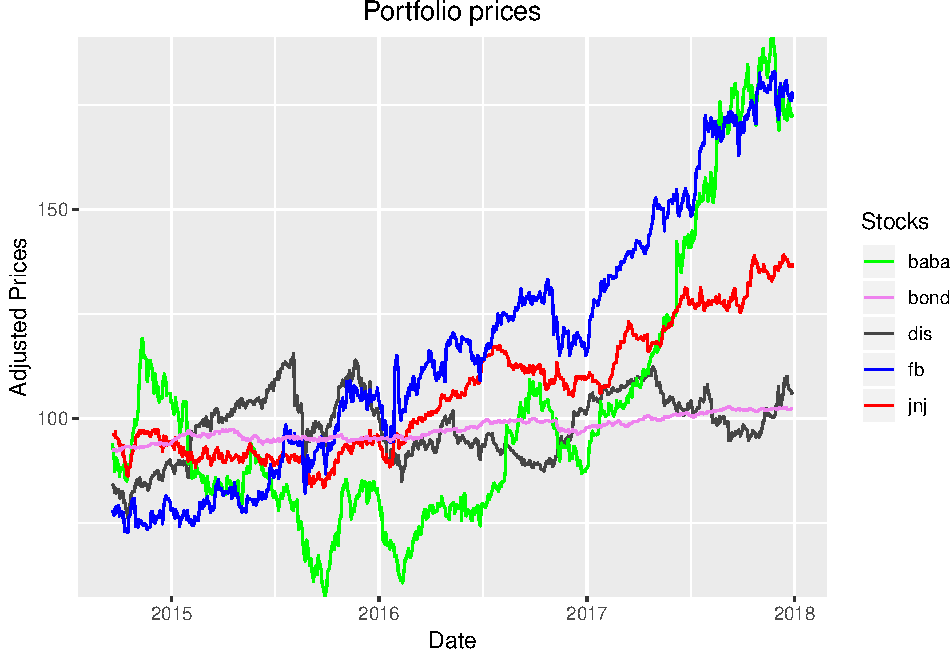
\includegraphics{Integrated_Management_Formulation_Model_files/figure-latex/unnamed-chunk-3-1.pdf}

We are going to look on the solution of the problem when gamma =
0.1,0.3,0.5,0.7 and 0.9 to understand the differences in these levels.

Solving the problem in linprog needs the definition of the Amat matrix,
object vector and the constraint vector as in \(Ax \leq b\) where \(A\)
is the Amat matrix, \(x\) is the vector to be solved and \(b\) is the
right hand solution. Object vector is deefined by the objective function
of the problem. ( see
\href{https://www.rdocumentation.org/packages/linprog/versions/0.9-2/topics/solveLP}{solveLP
function in R} from package \textbf{linprog}.)

We want to see what happens for the stocks in the changing levels of
\(\gamma\) as the levels of \(\alpha\) increases.

The \textbf{Amat} matrix doesn't change in all the levels of \(\gamma\)
and so once defined, we will just use the same matrix for all the
levels. The \textbf{cvec} vector changes and \textbf{bvec} vector
remains the same through all considered levels of \(\gamma\).

\subsubsection{With gamma=0.1}\label{with-gamma0.1}

\begin{Shaded}
\begin{Highlighting}[]
\NormalTok{gamma1 =}\StringTok{ }\FloatTok{0.1}
\NormalTok{alpha =}\StringTok{ }\KeywordTok{c}\NormalTok{(}\FloatTok{0.01}\NormalTok{,}\FloatTok{0.05}\NormalTok{,}\FloatTok{0.1}\NormalTok{,}\FloatTok{0.2}\NormalTok{,}\FloatTok{0.3}\NormalTok{,}\FloatTok{0.4}\NormalTok{,}\FloatTok{0.50}\NormalTok{,}\FloatTok{0.60}\NormalTok{,}\FloatTok{0.70}\NormalTok{,}\FloatTok{0.80}\NormalTok{,}\FloatTok{0.90}\NormalTok{,}\FloatTok{0.95}\NormalTok{,}\FloatTok{0.99}\NormalTok{)}
\CommentTok{#creating empty vectors to hold the results}
\NormalTok{dis_result =}\StringTok{ }\KeywordTok{vector}\NormalTok{(}\DataTypeTok{mode =} \StringTok{"numeric"}\NormalTok{)}
\NormalTok{baba_result =}\StringTok{ }\KeywordTok{vector}\NormalTok{(}\DataTypeTok{mode =} \StringTok{"numeric"}\NormalTok{)}
\NormalTok{jnj_result =}\StringTok{ }\KeywordTok{vector}\NormalTok{(}\DataTypeTok{mode =} \StringTok{"numeric"}\NormalTok{)}
\NormalTok{fb_result =}\StringTok{ }\KeywordTok{vector}\NormalTok{(}\DataTypeTok{mode =} \StringTok{"numeric"}\NormalTok{)}
\NormalTok{q_result =}\StringTok{ }\KeywordTok{vector}\NormalTok{(}\DataTypeTok{mode =} \StringTok{"numeric"}\NormalTok{)}
\NormalTok{solution1 =}\StringTok{ }\KeywordTok{vector}\NormalTok{(}\DataTypeTok{mode =} \StringTok{"numeric"}\NormalTok{)}
\CommentTok{#looping over all the levels of alpha and filling up the empty vectors}
\ControlFlowTok{for}\NormalTok{ (alp }\ControlFlowTok{in}\NormalTok{ alpha)\{}
\NormalTok{  objvect <-}\StringTok{ }\KeywordTok{c}\NormalTok{((}\DecValTok{1}\OperatorTok{-}\NormalTok{gamma1)}\OperatorTok{*}\KeywordTok{t}\NormalTok{(prob)}\OperatorTok\NormalTok{Portreturns,(}\OperatorTok{-}\NormalTok{gamma1}\OperatorTok{/}\NormalTok{(}\DecValTok{1}\OperatorTok{-}\NormalTok{alp))}\OperatorTok{*}\KeywordTok{t}\NormalTok{(prob),}\OperatorTok{-}\NormalTok{gamma1)}
  \KeywordTok{names}\NormalTok{(objvect)<-}\KeywordTok{c}\NormalTok{(}\StringTok{"dis"}\NormalTok{,}\StringTok{"baba"}\NormalTok{,}\StringTok{"jnj"}\NormalTok{,}\StringTok{"fb"}\NormalTok{,}\KeywordTok{rep}\NormalTok{(}\StringTok{"z"}\NormalTok{,}\DecValTok{826}\NormalTok{),}\StringTok{"q"}\NormalTok{) }
\NormalTok{  rhscons <-}\StringTok{ }\KeywordTok{c}\NormalTok{(}\KeywordTok{rep}\NormalTok{(}\DecValTok{0}\NormalTok{,}\DecValTok{826}\NormalTok{ ),}\DecValTok{1}\NormalTok{,}\KeywordTok{rep}\NormalTok{(}\DecValTok{0}\NormalTok{,}\DecValTok{830}\NormalTok{))}
  \CommentTok{#Construction of matrix Amat}
\NormalTok{  firstcons =}\StringTok{ }\KeywordTok{cbind}\NormalTok{(}\OperatorTok{-}\NormalTok{Portreturns,}\OperatorTok{-}\KeywordTok{diag}\NormalTok{(}\DecValTok{826}\NormalTok{),}\OperatorTok{-}\KeywordTok{rep}\NormalTok{(}\DecValTok{1}\NormalTok{,}\DecValTok{826}\NormalTok{))}
\NormalTok{  secondcons =}\StringTok{ }\NormalTok{(}\KeywordTok{c}\NormalTok{(}\KeywordTok{rep}\NormalTok{(}\DecValTok{1}\NormalTok{,}\DecValTok{4}\NormalTok{),}\KeywordTok{rep}\NormalTok{(}\DecValTok{0}\NormalTok{,}\DecValTok{827}\NormalTok{)))}
\NormalTok{  lessx =}\StringTok{ }\KeywordTok{cbind}\NormalTok{(}\OperatorTok{-}\KeywordTok{diag}\NormalTok{(}\DecValTok{4}\NormalTok{),}\KeywordTok{zeros}\NormalTok{(}\DecValTok{4}\NormalTok{,}\DecValTok{827}\NormalTok{))}
\NormalTok{  lessz =}\StringTok{ }\KeywordTok{cbind}\NormalTok{(}\KeywordTok{zeros}\NormalTok{(}\DecValTok{826}\NormalTok{,}\DecValTok{4}\NormalTok{),}\OperatorTok{-}\KeywordTok{diag}\NormalTok{(}\DecValTok{826}\NormalTok{),}\KeywordTok{rep}\NormalTok{(}\DecValTok{0}\NormalTok{,}\DecValTok{826}\NormalTok{))}
\NormalTok{  Amat =}\StringTok{ }\KeywordTok{rbind}\NormalTok{(firstcons,secondcons,lessx,lessz)}
  \KeywordTok{dim}\NormalTok{(Amat)}
  \KeywordTok{colnames}\NormalTok{(Amat) =}\StringTok{ }\OtherTok{NULL}
  \KeywordTok{rownames}\NormalTok{(Amat) =}\StringTok{ }\OtherTok{NULL}
\NormalTok{  Solution1 <-}\StringTok{ }\KeywordTok{solveLP}\NormalTok{(objvect,rhscons,Amat,}\DataTypeTok{maximum =} \OtherTok{TRUE}\NormalTok{,}
          \DataTypeTok{const.dir =} \KeywordTok{c}\NormalTok{(}\KeywordTok{rep}\NormalTok{(}\StringTok{"<="}\NormalTok{,}\DecValTok{826}\NormalTok{),}\StringTok{"="}\NormalTok{,}\KeywordTok{rep}\NormalTok{(}\StringTok{"<="}\NormalTok{,}\DecValTok{830}\NormalTok{)),}\DataTypeTok{lpSolve =} \OtherTok{TRUE}\NormalTok{)}
\NormalTok{  dis_result<-}\KeywordTok{append}\NormalTok{(dis_result,Solution1}\OperatorTok{$}\NormalTok{solution[}\DecValTok{1}\NormalTok{])}
\NormalTok{  baba_result<-}\StringTok{ }\KeywordTok{append}\NormalTok{(baba_result,Solution1}\OperatorTok{$}\NormalTok{solution[}\DecValTok{2}\NormalTok{])}
\NormalTok{  jnj_result<-}\KeywordTok{append}\NormalTok{(jnj_result,Solution1}\OperatorTok{$}\NormalTok{solution[}\DecValTok{3}\NormalTok{])}
\NormalTok{  fb_result<-}\KeywordTok{append}\NormalTok{(fb_result,Solution1}\OperatorTok{$}\NormalTok{solution[}\DecValTok{4}\NormalTok{])}
\NormalTok{  q_result <-}\StringTok{ }\KeywordTok{append}\NormalTok{(q_result,Solution1}\OperatorTok{$}\NormalTok{solution[}\DecValTok{831}\NormalTok{])}
\NormalTok{  solution1 <-}\StringTok{ }\KeywordTok{append}\NormalTok{(solution1,Solution1}\OperatorTok{$}\NormalTok{opt)}
\NormalTok{\}}
\end{Highlighting}
\end{Shaded}

The value \(q\) in the problem is the Value-at-Risk and so it is
important to look at it also.

\paragraph{Plot of alpha vs q
(Value-at-Risk)}\label{plot-of-alpha-vs-q-value-at-risk}

\begin{Shaded}
\begin{Highlighting}[]
\CommentTok{#creating a dataframe and writing the results into a CSV file}
\NormalTok{result_q <-}\StringTok{ }\KeywordTok{data.frame}\NormalTok{(alpha,q_result)}
\KeywordTok{write.csv}\NormalTok{(result_q,}\DataTypeTok{file =} \StringTok{"VaR_Results.csv"}\NormalTok{)}
\CommentTok{#Plotting}
\KeywordTok{ggplot}\NormalTok{(}\DataTypeTok{data=}\NormalTok{result_q, }\KeywordTok{aes}\NormalTok{(}\DataTypeTok{x=}\NormalTok{alpha, }\DataTypeTok{y=}\NormalTok{q_result, }\DataTypeTok{group=}\DecValTok{1}\NormalTok{)) }\OperatorTok{+}
\StringTok{  }\KeywordTok{geom_line}\NormalTok{(}\DataTypeTok{color=}\StringTok{"blue"}\NormalTok{)}\OperatorTok{+}
\StringTok{  }\KeywordTok{geom_point}\NormalTok{()}\OperatorTok{+}
\StringTok{  }\KeywordTok{labs}\NormalTok{(}\DataTypeTok{title=}\StringTok{"Plot of VaR vs Alpha for Gamma = 0.1 "}\NormalTok{,}\DataTypeTok{x=}\StringTok{"Value of Alpha"}\NormalTok{, }\DataTypeTok{y =} \StringTok{"Value At Risk"}\NormalTok{)}\OperatorTok{+}
\StringTok{  }\KeywordTok{theme_classic}\NormalTok{()}
\end{Highlighting}
\end{Shaded}

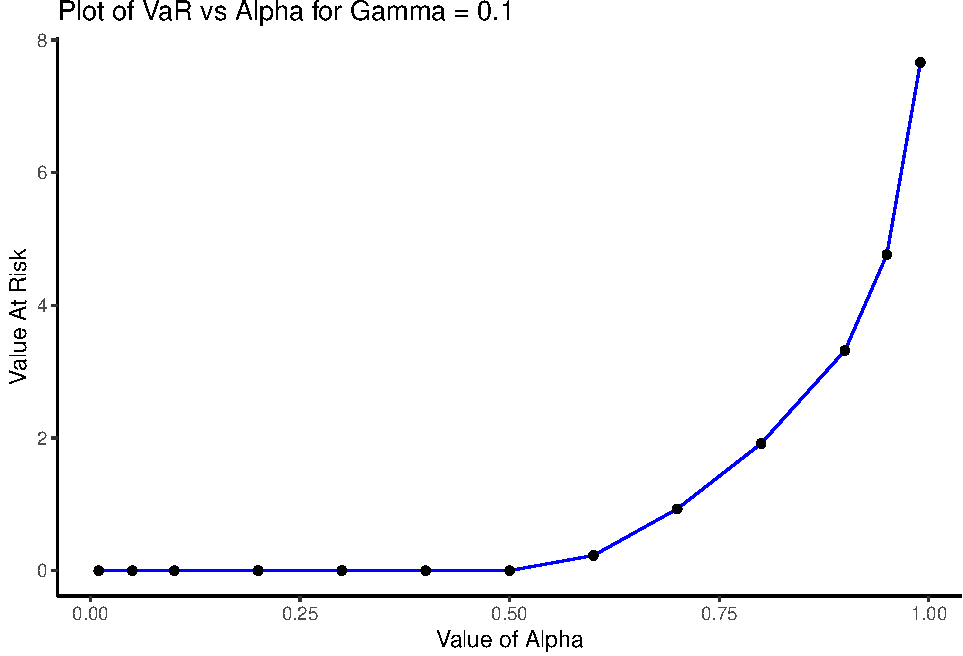
\includegraphics{Integrated_Management_Formulation_Model_files/figure-latex/unnamed-chunk-5-1.pdf}

It is important to look at the development of the optimal value in the
various levels of alpha also.

\paragraph{Plot of alpha vs optimal
value}\label{plot-of-alpha-vs-optimal-value}

\begin{Shaded}
\begin{Highlighting}[]
\NormalTok{result_sol <-}\StringTok{ }\KeywordTok{data.frame}\NormalTok{(alpha,solution1)}
\KeywordTok{write.csv}\NormalTok{(result_sol,}\DataTypeTok{file =} \StringTok{"Solution_fun.csv"}\NormalTok{)}
\KeywordTok{ggplot}\NormalTok{(}\DataTypeTok{data=}\NormalTok{result_sol, }\KeywordTok{aes}\NormalTok{(}\DataTypeTok{x=}\NormalTok{alpha, }\DataTypeTok{y=}\NormalTok{solution1, }\DataTypeTok{group=}\DecValTok{1}\NormalTok{)) }\OperatorTok{+}
\StringTok{  }\KeywordTok{geom_line}\NormalTok{(}\DataTypeTok{color=}\StringTok{"blue"}\NormalTok{)}\OperatorTok{+}
\StringTok{  }\KeywordTok{geom_point}\NormalTok{()}\OperatorTok{+}
\StringTok{  }\KeywordTok{labs}\NormalTok{(}\DataTypeTok{title=}\StringTok{"Plot of optimal value vs Alpha for Gamma = 0.1 "}\NormalTok{,}\DataTypeTok{x=}\StringTok{"Value of Alpha"}\NormalTok{, }\DataTypeTok{y =} \StringTok{"Function value"}\NormalTok{)}\OperatorTok{+}
\StringTok{  }\KeywordTok{theme_classic}\NormalTok{()}
\end{Highlighting}
\end{Shaded}

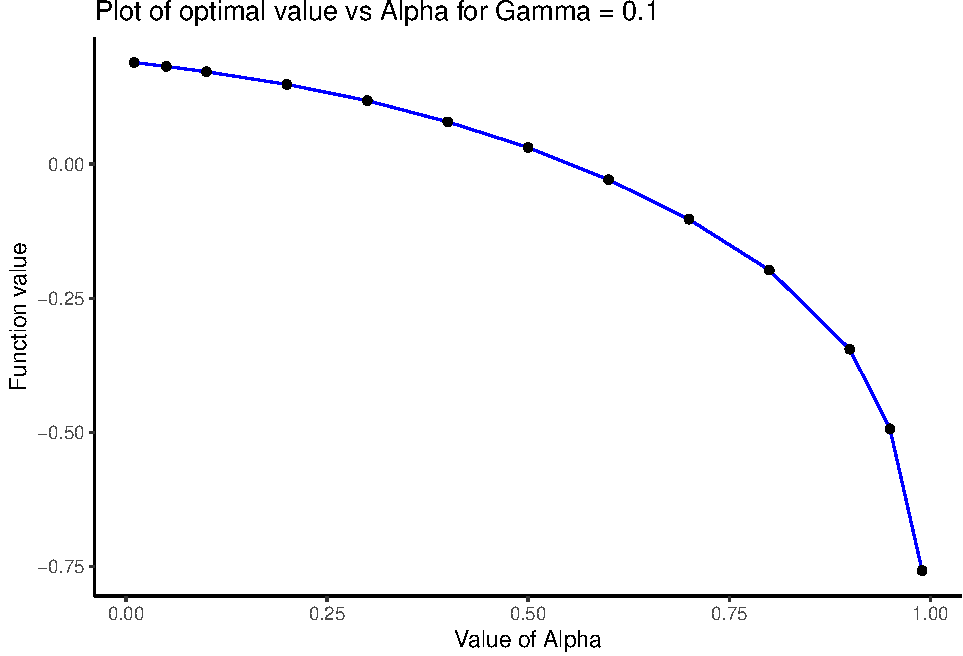
\includegraphics{Integrated_Management_Formulation_Model_files/figure-latex/unnamed-chunk-6-1.pdf}

The asset allocation weights of the problem wehn gamma = 0.1 is as
follows

\paragraph{\texorpdfstring{Asset allocation for
\(\gamma = 0.1\)}{Asset allocation for \textbackslash{}gamma = 0.1}}\label{asset-allocation-for-gamma-0.1}

\begin{Shaded}
\begin{Highlighting}[]
\NormalTok{result1 <-}\KeywordTok{data.frame}\NormalTok{(alpha,dis_result,baba_result,jnj_result,fb_result)}
\KeywordTok{write.csv}\NormalTok{(result1, }\DataTypeTok{file =} \StringTok{"Results1.csv"}\NormalTok{)}
\KeywordTok{ggplot}\NormalTok{(result1, }\KeywordTok{aes}\NormalTok{(}\DataTypeTok{x=}\NormalTok{result1}\OperatorTok{$}\NormalTok{alpha)) }\OperatorTok{+}\StringTok{ }
\StringTok{  }\KeywordTok{geom_area}\NormalTok{(}\KeywordTok{aes}\NormalTok{(}\DataTypeTok{y=}\NormalTok{result1}\OperatorTok{$}\NormalTok{dis_result}\OperatorTok{+}\NormalTok{result1}\OperatorTok{$}\NormalTok{baba_result}\OperatorTok{+}\NormalTok{result1}\OperatorTok{$}\NormalTok{jnj_result}\OperatorTok{+}
\StringTok{                  }\NormalTok{result1}\OperatorTok{$}\NormalTok{fb_result, }\DataTypeTok{fill=}\StringTok{"fb"}\NormalTok{))}\OperatorTok{+}
\StringTok{  }\KeywordTok{geom_area}\NormalTok{(}\KeywordTok{aes}\NormalTok{(}\DataTypeTok{y=}\NormalTok{result1}\OperatorTok{$}\NormalTok{dis_result}\OperatorTok{+}\NormalTok{result1}\OperatorTok{$}\NormalTok{baba_result}\OperatorTok{+}\NormalTok{result1}\OperatorTok{$}\NormalTok{jnj_result, }\DataTypeTok{fill=}\StringTok{"jnj"}\NormalTok{)) }\OperatorTok{+}
\StringTok{  }\KeywordTok{geom_area}\NormalTok{(}\KeywordTok{aes}\NormalTok{(}\DataTypeTok{y=}\NormalTok{result1}\OperatorTok{$}\NormalTok{dis_result}\OperatorTok{+}\NormalTok{result1}\OperatorTok{$}\NormalTok{baba_result, }\DataTypeTok{fill=}\StringTok{"baba"}\NormalTok{)) }\OperatorTok{+}
\StringTok{  }\KeywordTok{geom_area}\NormalTok{(}\KeywordTok{aes}\NormalTok{(}\DataTypeTok{y=}\NormalTok{result1}\OperatorTok{$}\NormalTok{dis_result,}\DataTypeTok{fill =} \StringTok{'dis'}\NormalTok{)) }\OperatorTok{+}\StringTok{ }
\StringTok{  }\KeywordTok{xlab}\NormalTok{(}\StringTok{"Alpha Values"}\NormalTok{) }\OperatorTok{+}\StringTok{ }\KeywordTok{ylab}\NormalTok{(}\StringTok{"Allocations to Stocks"}\NormalTok{) }\OperatorTok{+}
\StringTok{  }\KeywordTok{labs}\NormalTok{(}\DataTypeTok{title=}\StringTok{"Area plot for results when gamma = 0.1"}\NormalTok{) }\OperatorTok{+}
\StringTok{  }\KeywordTok{scale_fill_manual}\NormalTok{(}\StringTok{"Stocks"}\NormalTok{,}\DataTypeTok{values =}
                      \KeywordTok{c}\NormalTok{(}\StringTok{"fb"}\NormalTok{=}\StringTok{"#0000FF"}\NormalTok{,}\StringTok{"jnj"}\NormalTok{=}\StringTok{"#00FF00"}\NormalTok{,}\StringTok{"baba"}\NormalTok{=}\StringTok{"#FF0000"}\NormalTok{,}\StringTok{"dis"}\NormalTok{=}\StringTok{"#454545"}\NormalTok{))}
\end{Highlighting}
\end{Shaded}

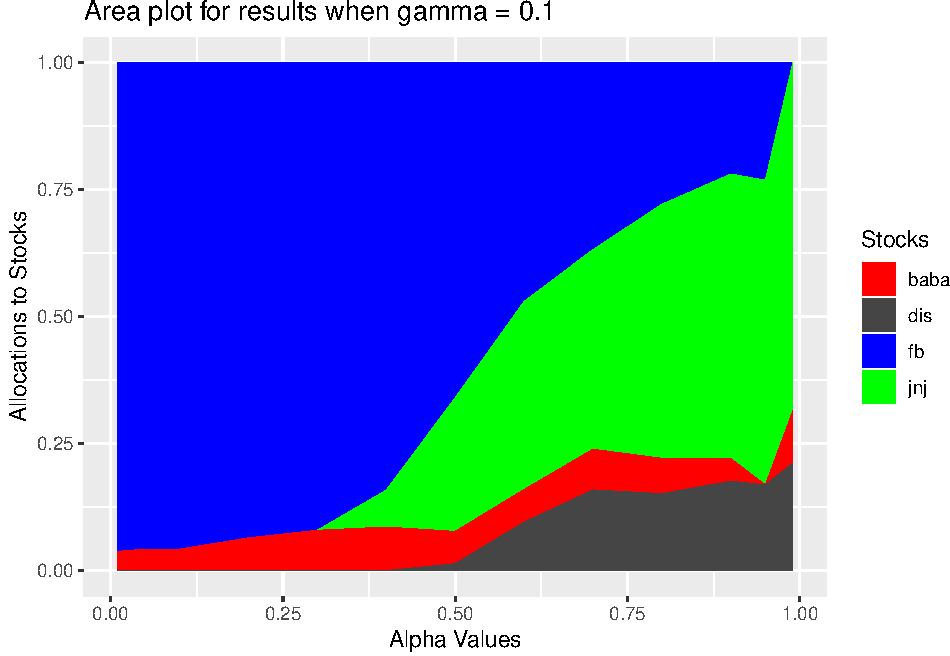
\includegraphics{Integrated_Management_Formulation_Model_files/figure-latex/unnamed-chunk-7-1.pdf}

\begin{Shaded}
\begin{Highlighting}[]
\CommentTok{# Using stacked barplots }
\KeywordTok{library}\NormalTok{(reshape2)}
\NormalTok{data1 <-}\StringTok{ }\NormalTok{result1}
\KeywordTok{names}\NormalTok{(data1) <-}\StringTok{ }\KeywordTok{c}\NormalTok{(}\StringTok{"alpha"}\NormalTok{,}\StringTok{"DIS"}\NormalTok{,}\StringTok{"BABA"}\NormalTok{,}\StringTok{"JNJ"}\NormalTok{,}\StringTok{"FB"}\NormalTok{)}
\NormalTok{mdata <-}\StringTok{ }\KeywordTok{melt}\NormalTok{(data1, }\DataTypeTok{id=}\KeywordTok{c}\NormalTok{(}\StringTok{"alpha"}\NormalTok{))}
\KeywordTok{names}\NormalTok{(mdata) <-}\StringTok{ }\KeywordTok{c}\NormalTok{(}\StringTok{"Alpha"}\NormalTok{,}\StringTok{"Stocks"}\NormalTok{,}\StringTok{"Allocation"}\NormalTok{)}
\KeywordTok{ggplot}\NormalTok{() }\OperatorTok{+}\StringTok{ }\KeywordTok{geom_bar}\NormalTok{(}\KeywordTok{aes}\NormalTok{(}\DataTypeTok{y =}\NormalTok{ Allocation, }\DataTypeTok{x =}\NormalTok{ Alpha, }\DataTypeTok{fill =}\NormalTok{ Stocks), }\DataTypeTok{data =}\NormalTok{ mdata, }\DataTypeTok{stat=}\StringTok{"identity"}\NormalTok{)}\OperatorTok{+}
\StringTok{  }\KeywordTok{scale_fill_manual}\NormalTok{(}\StringTok{"Stocks"}\NormalTok{,}\DataTypeTok{values =}
                      \KeywordTok{c}\NormalTok{(}\StringTok{"FB"}\NormalTok{=}\StringTok{"#0000FF"}\NormalTok{,}\StringTok{"JNJ"}\NormalTok{=}\StringTok{"#00FF00"}\NormalTok{,}\StringTok{"BABA"}\NormalTok{=}\StringTok{"#FF0000"}\NormalTok{,}\StringTok{"DIS"}\NormalTok{=}\StringTok{"#454545"}\NormalTok{))}
\end{Highlighting}
\end{Shaded}

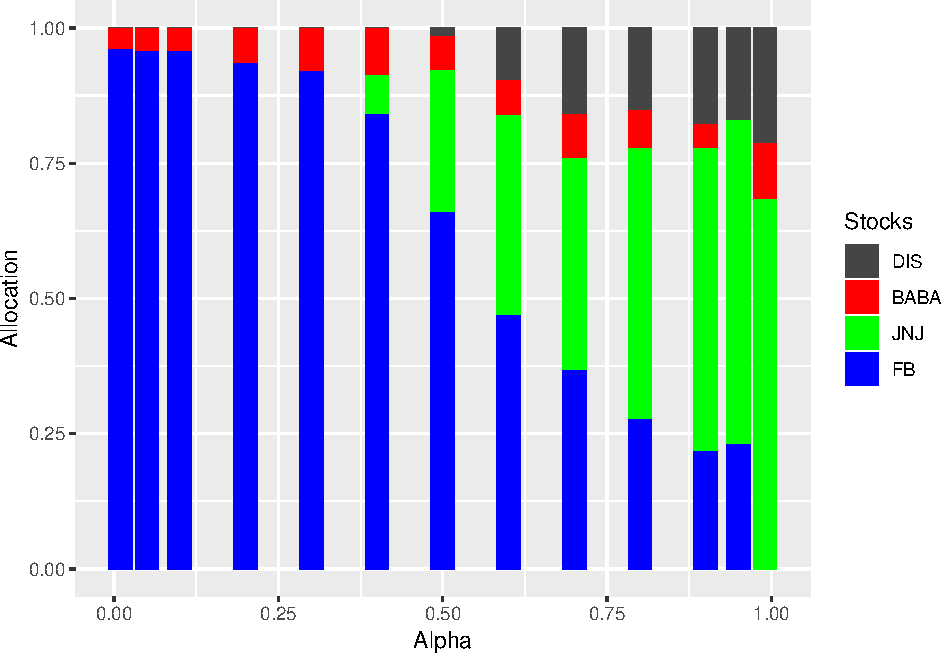
\includegraphics{Integrated_Management_Formulation_Model_files/figure-latex/unnamed-chunk-7-2.pdf}

\subsubsection{With gamma=0}\label{with-gamma0}

\begin{Shaded}
\begin{Highlighting}[]
\NormalTok{gamma0 =}\StringTok{ }\FloatTok{0.0}
\NormalTok{dis_result0 =}\StringTok{ }\KeywordTok{vector}\NormalTok{(}\DataTypeTok{mode =} \StringTok{"numeric"}\NormalTok{)}
\NormalTok{baba_result0 =}\StringTok{ }\KeywordTok{vector}\NormalTok{(}\DataTypeTok{mode =} \StringTok{"numeric"}\NormalTok{)}
\NormalTok{jnj_result0 =}\StringTok{ }\KeywordTok{vector}\NormalTok{(}\DataTypeTok{mode =} \StringTok{"numeric"}\NormalTok{)}
\NormalTok{fb_result0 =}\StringTok{ }\KeywordTok{vector}\NormalTok{(}\DataTypeTok{mode =} \StringTok{"numeric"}\NormalTok{)}
\NormalTok{q_result0 =}\StringTok{ }\KeywordTok{vector}\NormalTok{(}\DataTypeTok{mode =} \StringTok{"numeric"}\NormalTok{)}
\ControlFlowTok{for}\NormalTok{ (alp }\ControlFlowTok{in}\NormalTok{ alpha)\{}
\NormalTok{  objvect0 <-}\StringTok{ }\KeywordTok{c}\NormalTok{((}\DecValTok{1}\OperatorTok{-}\NormalTok{gamma0)}\OperatorTok{*}\KeywordTok{t}\NormalTok{(prob)}\OperatorTok\NormalTok{Portreturns,(}\OperatorTok{-}\NormalTok{gamma0}\OperatorTok{/}\NormalTok{(}\DecValTok{1}\OperatorTok{-}\NormalTok{alp))}\OperatorTok{*}\KeywordTok{t}\NormalTok{(prob),}\OperatorTok{-}\NormalTok{gamma0)}
  \KeywordTok{names}\NormalTok{(objvect0)<-}\KeywordTok{c}\NormalTok{(}\StringTok{"dis"}\NormalTok{,}\StringTok{"baba"}\NormalTok{,}\StringTok{"jnj"}\NormalTok{,}\StringTok{"fb"}\NormalTok{,}\KeywordTok{rep}\NormalTok{(}\StringTok{"z"}\NormalTok{,}\DecValTok{826}\NormalTok{),}\StringTok{"q"}\NormalTok{)}
  
\NormalTok{  Solution0 <-}\StringTok{ }\KeywordTok{solveLP}\NormalTok{(objvect0,rhscons,Amat,}\DataTypeTok{maximum =} \OtherTok{TRUE}\NormalTok{,}
          \DataTypeTok{const.dir =} \KeywordTok{c}\NormalTok{(}\KeywordTok{rep}\NormalTok{(}\StringTok{"<="}\NormalTok{,}\DecValTok{826}\NormalTok{),}\StringTok{"="}\NormalTok{,}\KeywordTok{rep}\NormalTok{(}\StringTok{"<="}\NormalTok{,}\DecValTok{830}\NormalTok{)),}\DataTypeTok{lpSolve =} \OtherTok{TRUE}\NormalTok{)}
\NormalTok{  dis_result0 <-}\StringTok{ }\KeywordTok{append}\NormalTok{(dis_result0,Solution0}\OperatorTok{$}\NormalTok{solution[}\DecValTok{1}\NormalTok{])}
\NormalTok{  baba_result0 <-}\StringTok{ }\KeywordTok{append}\NormalTok{(baba_result0,Solution0}\OperatorTok{$}\NormalTok{solution[}\DecValTok{2}\NormalTok{])}
\NormalTok{  jnj_result0 <-}\StringTok{ }\KeywordTok{append}\NormalTok{(jnj_result0,Solution0}\OperatorTok{$}\NormalTok{solution[}\DecValTok{3}\NormalTok{])}
\NormalTok{  fb_result0<-}\StringTok{ }\KeywordTok{append}\NormalTok{(fb_result0,Solution0}\OperatorTok{$}\NormalTok{solution[}\DecValTok{4}\NormalTok{])}
\NormalTok{  q_result0 <-}\StringTok{ }\KeywordTok{append}\NormalTok{(q_result0,Solution0}\OperatorTok{$}\NormalTok{solution[}\DecValTok{831}\NormalTok{])}
\NormalTok{\}}
\end{Highlighting}
\end{Shaded}

\subsubsection{\texorpdfstring{Asset allocation for
\(\gamma=0.0\)}{Asset allocation for \textbackslash{}gamma=0.0}}\label{asset-allocation-for-gamma0.0}

\begin{Shaded}
\begin{Highlighting}[]
\NormalTok{result0 <-}\StringTok{  }\KeywordTok{data.frame}\NormalTok{(alpha,dis_result0,baba_result0,jnj_result0,fb_result0)}
\KeywordTok{write.csv}\NormalTok{(result0, }\DataTypeTok{file =} \StringTok{"Results0.csv"}\NormalTok{)}
\KeywordTok{ggplot}\NormalTok{(result0, }\KeywordTok{aes}\NormalTok{(}\DataTypeTok{x=}\NormalTok{result0}\OperatorTok{$}\NormalTok{alpha)) }\OperatorTok{+}\StringTok{ }
\StringTok{  }\KeywordTok{geom_area}\NormalTok{(}\KeywordTok{aes}\NormalTok{(}\DataTypeTok{y=}\NormalTok{result0}\OperatorTok{$}\NormalTok{dis_result0}\OperatorTok{+}\NormalTok{result0}\OperatorTok{$}\NormalTok{baba_result0}\OperatorTok{+}\NormalTok{result0}\OperatorTok{$}\NormalTok{jnj_result0}\OperatorTok{+}\NormalTok{result0}\OperatorTok{$}\NormalTok{fb_result0, }\DataTypeTok{fill=}\StringTok{"fb"}\NormalTok{))}\OperatorTok{+}
\StringTok{  }\KeywordTok{geom_area}\NormalTok{(}\KeywordTok{aes}\NormalTok{(}\DataTypeTok{y=}\NormalTok{result0}\OperatorTok{$}\NormalTok{dis_result0}\OperatorTok{+}\NormalTok{result0}\OperatorTok{$}\NormalTok{baba_result0}\OperatorTok{+}\NormalTok{result0}\OperatorTok{$}\NormalTok{jnj_result0, }\DataTypeTok{fill=}\StringTok{"jnj"}\NormalTok{)) }\OperatorTok{+}
\StringTok{  }\KeywordTok{geom_area}\NormalTok{(}\KeywordTok{aes}\NormalTok{(}\DataTypeTok{y=}\NormalTok{result0}\OperatorTok{$}\NormalTok{dis_result0}\OperatorTok{+}\NormalTok{result0}\OperatorTok{$}\NormalTok{baba_result0, }\DataTypeTok{fill=}\StringTok{"baba"}\NormalTok{)) }\OperatorTok{+}
\StringTok{  }\KeywordTok{geom_area}\NormalTok{(}\KeywordTok{aes}\NormalTok{(}\DataTypeTok{y=}\NormalTok{result0}\OperatorTok{$}\NormalTok{dis_result0,}\DataTypeTok{fill =} \StringTok{'dis'}\NormalTok{)) }\OperatorTok{+}\StringTok{ }
\StringTok{  }\KeywordTok{xlab}\NormalTok{(}\StringTok{"Alpha Values"}\NormalTok{) }\OperatorTok{+}\StringTok{ }\KeywordTok{ylab}\NormalTok{(}\StringTok{"Allocations to Stocks"}\NormalTok{) }\OperatorTok{+}
\StringTok{  }\KeywordTok{labs}\NormalTok{(}\DataTypeTok{title=}\StringTok{"Area plot for gamma = 0"}\NormalTok{) }\OperatorTok{+}\StringTok{  }\CommentTok{# title and caption}
\StringTok{  }\KeywordTok{scale_fill_manual}\NormalTok{(}\StringTok{"Stocks"}\NormalTok{,}\DataTypeTok{values =} \KeywordTok{c}\NormalTok{(}\StringTok{"fb"}\NormalTok{=}\StringTok{"#0000FF"}\NormalTok{,}\StringTok{"jnj"}\NormalTok{=}\StringTok{"#00FF00"}\NormalTok{,}\StringTok{"baba"}\NormalTok{=}\StringTok{"#FF0000"}\NormalTok{,}\StringTok{"dis"}\NormalTok{=}\StringTok{"#454545"}\NormalTok{)) }
\end{Highlighting}
\end{Shaded}

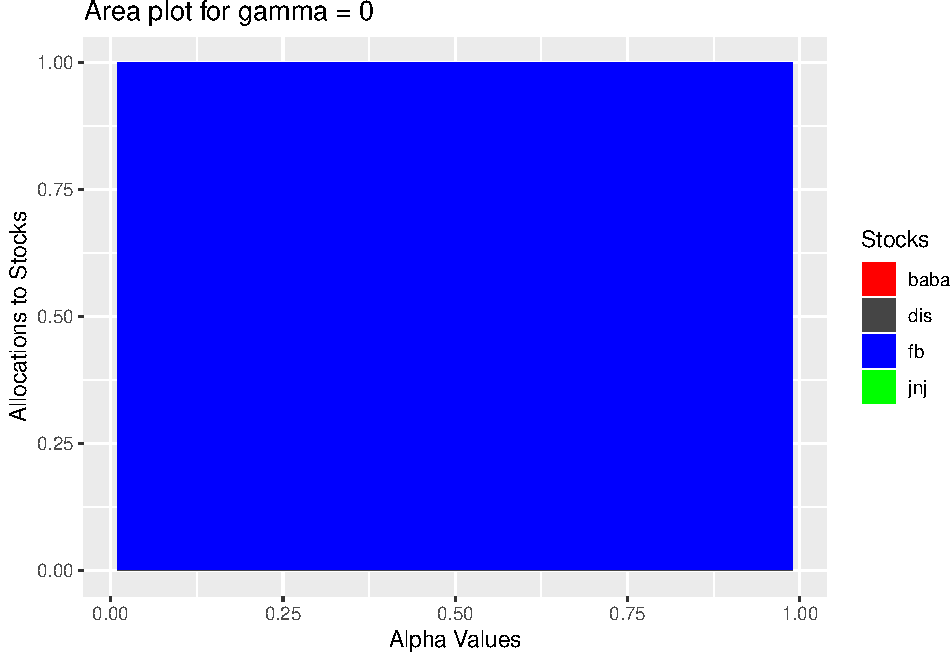
\includegraphics{Integrated_Management_Formulation_Model_files/figure-latex/unnamed-chunk-9-1.pdf}

Note that the choice \(\gamma = 0\) identifies the stock with the
highest return during the considered period and puts all possible
weights onto this stock. In this case, the stock itself is FB.

\paragraph{Plot of alpha vs q for gamma =
0}\label{plot-of-alpha-vs-q-for-gamma-0}

\begin{Shaded}
\begin{Highlighting}[]
\NormalTok{result_q0 <-}\StringTok{ }\KeywordTok{data.frame}\NormalTok{(alpha,q_result0)}
\KeywordTok{write.csv}\NormalTok{(result_q0,}\DataTypeTok{file =} \StringTok{"VaR_Results0.csv"}\NormalTok{)}
\KeywordTok{ggplot}\NormalTok{(}\DataTypeTok{data=}\NormalTok{result_q0, }\KeywordTok{aes}\NormalTok{(}\DataTypeTok{x=}\NormalTok{alpha, }\DataTypeTok{y=}\NormalTok{q_result0, }\DataTypeTok{group=}\DecValTok{1}\NormalTok{)) }\OperatorTok{+}
\StringTok{  }\KeywordTok{geom_line}\NormalTok{(}\DataTypeTok{color=}\StringTok{"blue"}\NormalTok{)}\OperatorTok{+}
\StringTok{  }\KeywordTok{geom_point}\NormalTok{()}\OperatorTok{+}
\StringTok{  }\KeywordTok{labs}\NormalTok{(}\DataTypeTok{title=}\StringTok{"Plot of VaR vs Alpha for Gamma = 0.0 "}\NormalTok{,}\DataTypeTok{x=}\StringTok{"Value of Alpha"}\NormalTok{, }\DataTypeTok{y =} \StringTok{"Value At Risk"}\NormalTok{)}\OperatorTok{+}
\StringTok{  }\KeywordTok{theme_classic}\NormalTok{()}
\end{Highlighting}
\end{Shaded}

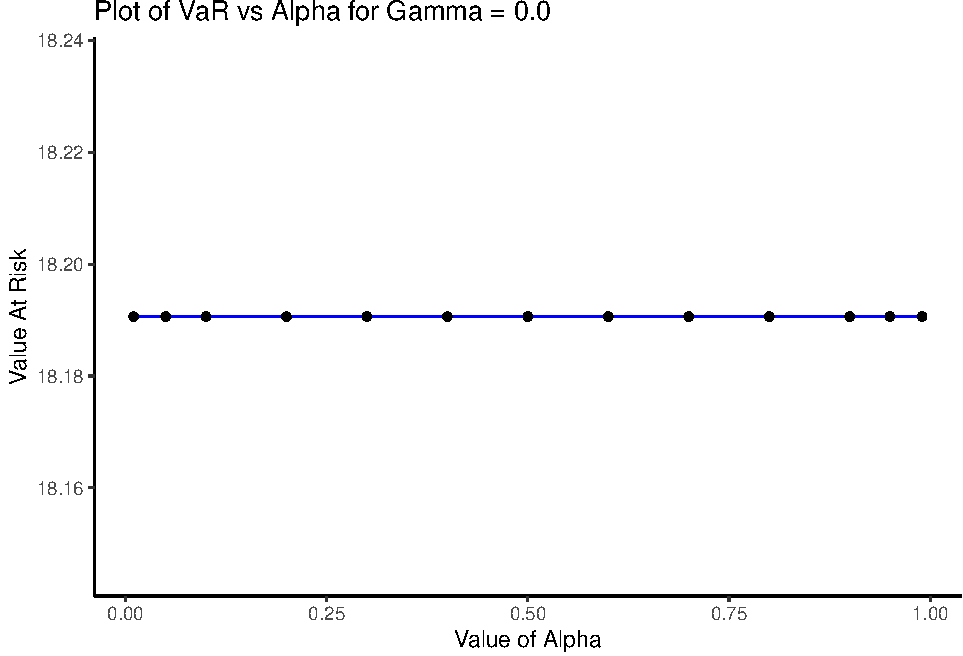
\includegraphics{Integrated_Management_Formulation_Model_files/figure-latex/unnamed-chunk-10-1.pdf}

\subsubsection{With gamma = 0.3}\label{with-gamma-0.3}

\begin{Shaded}
\begin{Highlighting}[]
\NormalTok{gamma3 =}\StringTok{ }\FloatTok{0.3}
\NormalTok{dis_result3 =}\StringTok{ }\KeywordTok{vector}\NormalTok{(}\DataTypeTok{mode =} \StringTok{"numeric"}\NormalTok{)}
\NormalTok{baba_result3 =}\StringTok{ }\KeywordTok{vector}\NormalTok{(}\DataTypeTok{mode =} \StringTok{"numeric"}\NormalTok{)}
\NormalTok{jnj_result3 =}\StringTok{ }\KeywordTok{vector}\NormalTok{(}\DataTypeTok{mode =} \StringTok{"numeric"}\NormalTok{)}
\NormalTok{fb_result3 =}\StringTok{ }\KeywordTok{vector}\NormalTok{(}\DataTypeTok{mode =} \StringTok{"numeric"}\NormalTok{)}
\NormalTok{q_result3 =}\StringTok{ }\KeywordTok{vector}\NormalTok{(}\DataTypeTok{mode =} \StringTok{"numeric"}\NormalTok{)}
\ControlFlowTok{for}\NormalTok{ (alp }\ControlFlowTok{in}\NormalTok{ alpha)\{}
\NormalTok{  objvect3 <-}\StringTok{ }\KeywordTok{c}\NormalTok{((}\DecValTok{1}\OperatorTok{-}\NormalTok{gamma3)}\OperatorTok{*}\KeywordTok{t}\NormalTok{(prob)}\OperatorTok\NormalTok{Portreturns,(}\OperatorTok{-}\NormalTok{gamma3}\OperatorTok{/}\NormalTok{(}\DecValTok{1}\OperatorTok{-}\NormalTok{alp))}\OperatorTok{*}\KeywordTok{t}\NormalTok{(prob),}\OperatorTok{-}\NormalTok{gamma3)}
  \KeywordTok{names}\NormalTok{(objvect3)<-}\KeywordTok{c}\NormalTok{(}\StringTok{"dis"}\NormalTok{,}\StringTok{"baba"}\NormalTok{,}\StringTok{"jnj"}\NormalTok{,}\StringTok{"fb"}\NormalTok{,}\KeywordTok{rep}\NormalTok{(}\StringTok{"z"}\NormalTok{,}\DecValTok{826}\NormalTok{),}\StringTok{"q"}\NormalTok{) }
\NormalTok{  Solution3 <-}\StringTok{ }\KeywordTok{solveLP}\NormalTok{(objvect3,rhscons,Amat,}\DataTypeTok{maximum =} \OtherTok{TRUE}\NormalTok{,}
          \DataTypeTok{const.dir =} \KeywordTok{c}\NormalTok{(}\KeywordTok{rep}\NormalTok{(}\StringTok{"<="}\NormalTok{,}\DecValTok{826}\NormalTok{),}\StringTok{"="}\NormalTok{,}\KeywordTok{rep}\NormalTok{(}\StringTok{"<="}\NormalTok{,}\DecValTok{830}\NormalTok{)),}\DataTypeTok{lpSolve =} \OtherTok{TRUE}\NormalTok{)}
\NormalTok{  dis_result3 <-}\StringTok{ }\KeywordTok{append}\NormalTok{(dis_result3,Solution3}\OperatorTok{$}\NormalTok{solution[}\DecValTok{1}\NormalTok{])}
\NormalTok{  baba_result3 <-}\StringTok{ }\KeywordTok{append}\NormalTok{(baba_result3,Solution3}\OperatorTok{$}\NormalTok{solution[}\DecValTok{2}\NormalTok{])}
\NormalTok{  jnj_result3 <-}\StringTok{ }\KeywordTok{append}\NormalTok{(jnj_result3,Solution3}\OperatorTok{$}\NormalTok{solution[}\DecValTok{3}\NormalTok{])}
\NormalTok{  fb_result3<-}\StringTok{ }\KeywordTok{append}\NormalTok{(fb_result3,Solution3}\OperatorTok{$}\NormalTok{solution[}\DecValTok{4}\NormalTok{])}
\NormalTok{  q_result3 <-}\StringTok{ }\KeywordTok{append}\NormalTok{(q_result3,Solution3}\OperatorTok{$}\NormalTok{solution[}\DecValTok{831}\NormalTok{])}
\NormalTok{\}}
\end{Highlighting}
\end{Shaded}

\paragraph{\texorpdfstring{Asset allocation for
\(\gamma=0.3\)}{Asset allocation for \textbackslash{}gamma=0.3}}\label{asset-allocation-for-gamma0.3}

\begin{Shaded}
\begin{Highlighting}[]
\NormalTok{result3 <-}\StringTok{  }\KeywordTok{data.frame}\NormalTok{(alpha,dis_result3,baba_result3,jnj_result3,fb_result3)}
\KeywordTok{write.csv}\NormalTok{(result3, }\DataTypeTok{file =} \StringTok{"Results3.csv"}\NormalTok{)}
\KeywordTok{ggplot}\NormalTok{(result3, }\KeywordTok{aes}\NormalTok{(}\DataTypeTok{x=}\NormalTok{result3}\OperatorTok{$}\NormalTok{alpha)) }\OperatorTok{+}\StringTok{ }
\StringTok{  }\KeywordTok{geom_area}\NormalTok{(}\KeywordTok{aes}\NormalTok{(}\DataTypeTok{y=}\NormalTok{result3}\OperatorTok{$}\NormalTok{dis_result3}\OperatorTok{+}\NormalTok{result3}\OperatorTok{$}\NormalTok{baba_result3}\OperatorTok{+}\NormalTok{result3}\OperatorTok{$}\NormalTok{jnj_result3}\OperatorTok{+}\NormalTok{result3}\OperatorTok{$}\NormalTok{fb_result3, }\DataTypeTok{fill=}\StringTok{"fb"}\NormalTok{))}\OperatorTok{+}
\StringTok{  }\KeywordTok{geom_area}\NormalTok{(}\KeywordTok{aes}\NormalTok{(}\DataTypeTok{y=}\NormalTok{result3}\OperatorTok{$}\NormalTok{dis_result3}\OperatorTok{+}\NormalTok{result3}\OperatorTok{$}\NormalTok{baba_result3}\OperatorTok{+}\NormalTok{result3}\OperatorTok{$}\NormalTok{jnj_result3, }\DataTypeTok{fill=}\StringTok{"jnj"}\NormalTok{)) }\OperatorTok{+}
\StringTok{  }\KeywordTok{geom_area}\NormalTok{(}\KeywordTok{aes}\NormalTok{(}\DataTypeTok{y=}\NormalTok{result3}\OperatorTok{$}\NormalTok{dis_result3}\OperatorTok{+}\NormalTok{result3}\OperatorTok{$}\NormalTok{baba_result3, }\DataTypeTok{fill=}\StringTok{"baba"}\NormalTok{)) }\OperatorTok{+}
\StringTok{  }\KeywordTok{geom_area}\NormalTok{(}\KeywordTok{aes}\NormalTok{(}\DataTypeTok{y=}\NormalTok{result3}\OperatorTok{$}\NormalTok{dis_result3,}\DataTypeTok{fill =} \StringTok{'dis'}\NormalTok{)) }\OperatorTok{+}\StringTok{ }
\StringTok{  }\KeywordTok{xlab}\NormalTok{(}\StringTok{"Alpha Values"}\NormalTok{) }\OperatorTok{+}\StringTok{ }\KeywordTok{ylab}\NormalTok{(}\StringTok{"Allocations values"}\NormalTok{) }\OperatorTok{+}
\StringTok{  }\KeywordTok{labs}\NormalTok{(}\DataTypeTok{title=}\StringTok{"Area plot for gamma = 0.3"}\NormalTok{) }\OperatorTok{+}\StringTok{  }\CommentTok{# title and caption}
\StringTok{  }\KeywordTok{scale_fill_manual}\NormalTok{(}\StringTok{"Stocks"}\NormalTok{,}\DataTypeTok{values =} \KeywordTok{c}\NormalTok{(}\StringTok{"fb"}\NormalTok{=}\StringTok{"#0000FF"}\NormalTok{,}\StringTok{"jnj"}\NormalTok{=}\StringTok{"#00FF00"}\NormalTok{,}\StringTok{"baba"}\NormalTok{=}\StringTok{"#FF0000"}\NormalTok{,}\StringTok{"dis"}\NormalTok{=}\StringTok{"#454545"}\NormalTok{)) }
\end{Highlighting}
\end{Shaded}

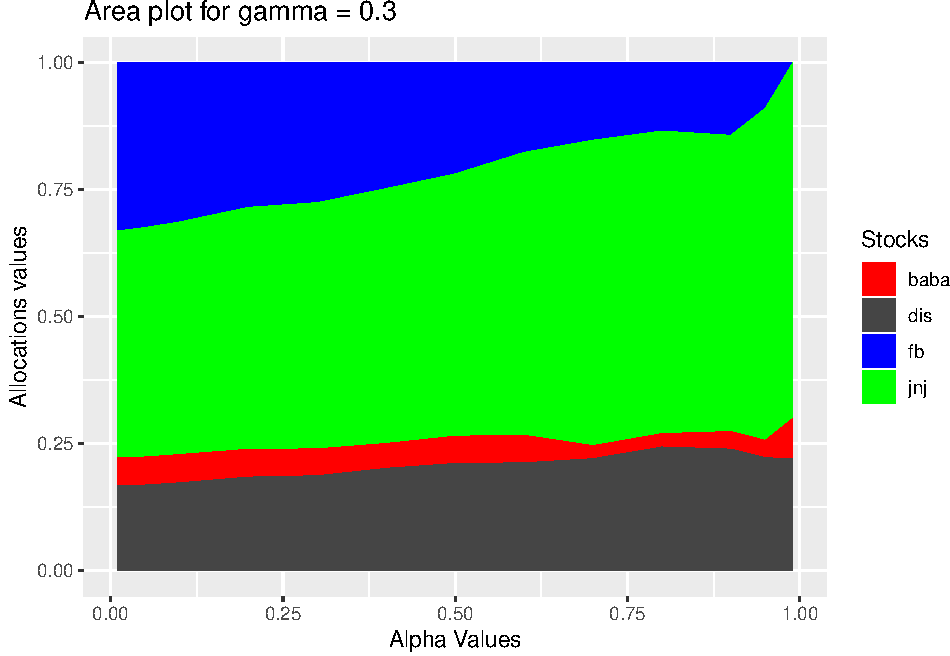
\includegraphics{Integrated_Management_Formulation_Model_files/figure-latex/unnamed-chunk-12-1.pdf}

\begin{Shaded}
\begin{Highlighting}[]
\NormalTok{data3 <-}\StringTok{ }\NormalTok{result3}
\KeywordTok{names}\NormalTok{(data3) <-}\StringTok{ }\KeywordTok{c}\NormalTok{(}\StringTok{"alpha"}\NormalTok{,}\StringTok{"DIS"}\NormalTok{,}\StringTok{"BABA"}\NormalTok{,}\StringTok{"JNJ"}\NormalTok{,}\StringTok{"FB"}\NormalTok{)}
\NormalTok{mdata3 <-}\StringTok{ }\KeywordTok{melt}\NormalTok{(data3, }\DataTypeTok{id=}\KeywordTok{c}\NormalTok{(}\StringTok{"alpha"}\NormalTok{))}
\KeywordTok{names}\NormalTok{(mdata3) <-}\StringTok{ }\KeywordTok{c}\NormalTok{(}\StringTok{"Alpha"}\NormalTok{,}\StringTok{"Stocks"}\NormalTok{,}\StringTok{"Allocation"}\NormalTok{)}
\KeywordTok{ggplot}\NormalTok{() }\OperatorTok{+}\StringTok{ }\KeywordTok{geom_bar}\NormalTok{(}\KeywordTok{aes}\NormalTok{(}\DataTypeTok{y =}\NormalTok{ Allocation, }\DataTypeTok{x =}\NormalTok{ Alpha, }\DataTypeTok{fill =}\NormalTok{ Stocks), }\DataTypeTok{data =}\NormalTok{ mdata3, }\DataTypeTok{stat=}\StringTok{"identity"}\NormalTok{)}\OperatorTok{+}
\StringTok{  }\KeywordTok{scale_fill_manual}\NormalTok{(}\StringTok{"Stocks"}\NormalTok{,}\DataTypeTok{values =}
                      \KeywordTok{c}\NormalTok{(}\StringTok{"FB"}\NormalTok{=}\StringTok{"#0000FF"}\NormalTok{,}\StringTok{"JNJ"}\NormalTok{=}\StringTok{"#00FF00"}\NormalTok{,}\StringTok{"BABA"}\NormalTok{=}\StringTok{"#FF0000"}\NormalTok{,}\StringTok{"DIS"}\NormalTok{=}\StringTok{"#454545"}\NormalTok{)) }
\end{Highlighting}
\end{Shaded}

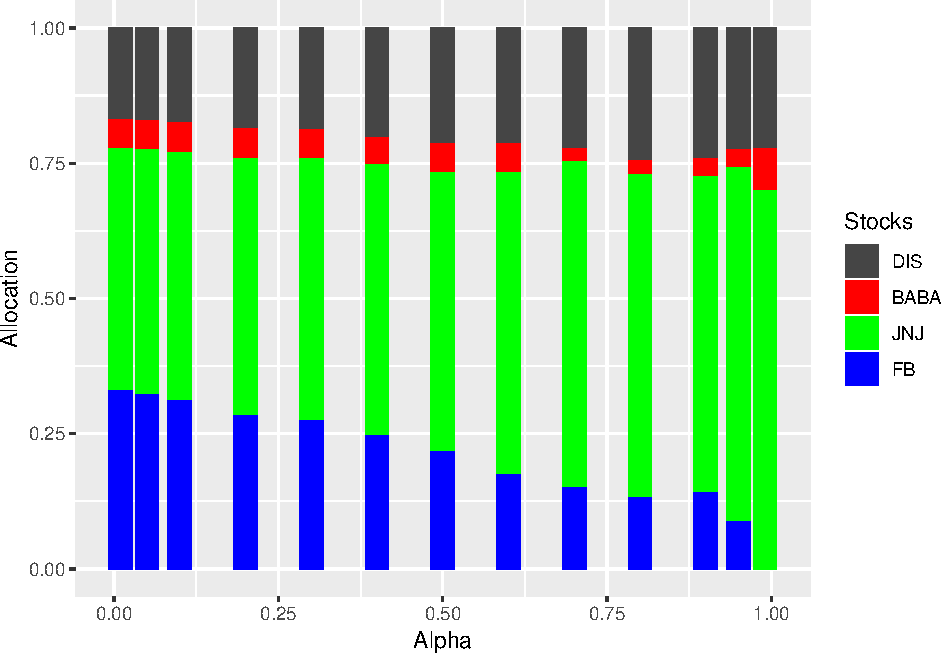
\includegraphics{Integrated_Management_Formulation_Model_files/figure-latex/unnamed-chunk-12-2.pdf}

\paragraph{Plot of alpha vs q for gamma =
0.3}\label{plot-of-alpha-vs-q-for-gamma-0.3}

\begin{Shaded}
\begin{Highlighting}[]
\NormalTok{result_q3 <-}\StringTok{ }\KeywordTok{data.frame}\NormalTok{(alpha,q_result3)}
\KeywordTok{write.csv}\NormalTok{(result_q3,}\DataTypeTok{file =} \StringTok{"VaR_Results3.csv"}\NormalTok{)}
\KeywordTok{ggplot}\NormalTok{(}\DataTypeTok{data=}\NormalTok{result_q3, }\KeywordTok{aes}\NormalTok{(}\DataTypeTok{x=}\NormalTok{alpha, }\DataTypeTok{y=}\NormalTok{q_result3, }\DataTypeTok{group=}\DecValTok{1}\NormalTok{)) }\OperatorTok{+}
\StringTok{  }\KeywordTok{geom_line}\NormalTok{(}\DataTypeTok{color=}\StringTok{"blue"}\NormalTok{)}\OperatorTok{+}
\StringTok{  }\KeywordTok{geom_point}\NormalTok{()}\OperatorTok{+}
\StringTok{  }\KeywordTok{labs}\NormalTok{(}\DataTypeTok{title=}\StringTok{"Plot of VaR vs Alpha for Gamma = 0.3 "}\NormalTok{,}\DataTypeTok{x=}\StringTok{"Value of Alpha"}\NormalTok{, }\DataTypeTok{y =} \StringTok{"Value At Risk"}\NormalTok{)}\OperatorTok{+}
\StringTok{  }\KeywordTok{theme_classic}\NormalTok{()}
\end{Highlighting}
\end{Shaded}

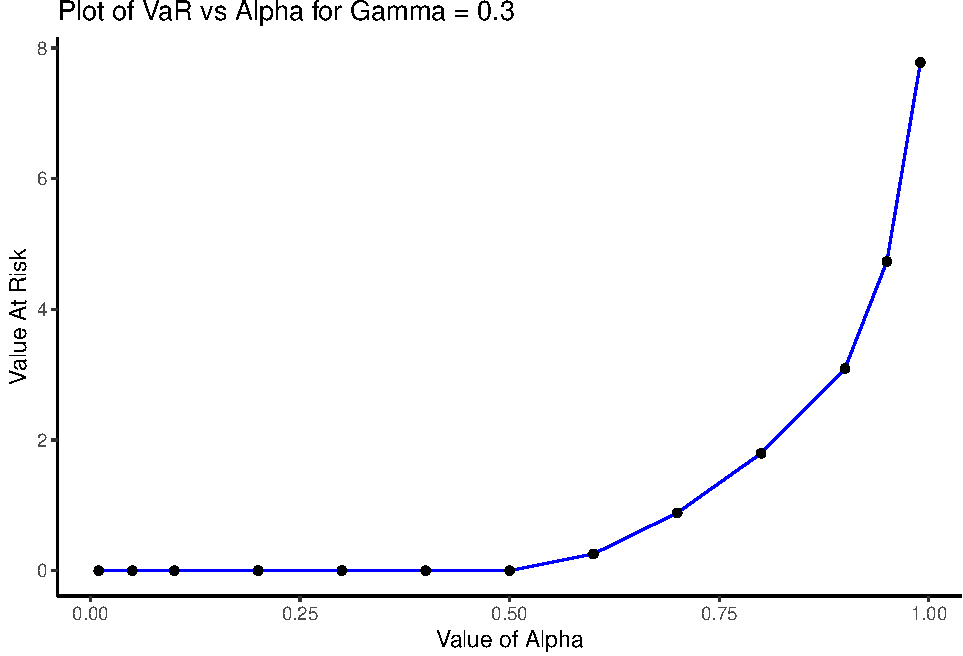
\includegraphics{Integrated_Management_Formulation_Model_files/figure-latex/unnamed-chunk-13-1.pdf}

\subsubsection{With gamma=0.5}\label{with-gamma0.5}

\begin{Shaded}
\begin{Highlighting}[]
\NormalTok{gamma5 =}\StringTok{ }\FloatTok{0.5}
\NormalTok{dis_result5 =}\StringTok{ }\KeywordTok{vector}\NormalTok{(}\DataTypeTok{mode =} \StringTok{"numeric"}\NormalTok{)}
\NormalTok{baba_result5 =}\StringTok{ }\KeywordTok{vector}\NormalTok{(}\DataTypeTok{mode =} \StringTok{"numeric"}\NormalTok{)}
\NormalTok{jnj_result5 =}\StringTok{ }\KeywordTok{vector}\NormalTok{(}\DataTypeTok{mode =} \StringTok{"numeric"}\NormalTok{)}
\NormalTok{fb_result5 =}\StringTok{ }\KeywordTok{vector}\NormalTok{(}\DataTypeTok{mode =} \StringTok{"numeric"}\NormalTok{)}
\NormalTok{q_result5 =}\StringTok{ }\KeywordTok{vector}\NormalTok{(}\DataTypeTok{mode =} \StringTok{"numeric"}\NormalTok{)}
\ControlFlowTok{for}\NormalTok{ (alp }\ControlFlowTok{in}\NormalTok{ alpha)\{}
\NormalTok{  objvect5 <-}\StringTok{ }\KeywordTok{c}\NormalTok{((}\DecValTok{1}\OperatorTok{-}\NormalTok{gamma5)}\OperatorTok{*}\KeywordTok{t}\NormalTok{(prob)}\OperatorTok\NormalTok{Portreturns,(}\OperatorTok{-}\NormalTok{gamma5}\OperatorTok{/}\NormalTok{(}\DecValTok{1}\OperatorTok{-}\NormalTok{alp))}\OperatorTok{*}\KeywordTok{t}\NormalTok{(prob),}\OperatorTok{-}\NormalTok{gamma5)}
  \KeywordTok{names}\NormalTok{(objvect5)<-}\KeywordTok{c}\NormalTok{(}\StringTok{"dis"}\NormalTok{,}\StringTok{"baba"}\NormalTok{,}\StringTok{"jnj"}\NormalTok{,}\StringTok{"fb"}\NormalTok{,}\KeywordTok{rep}\NormalTok{(}\StringTok{"z"}\NormalTok{,}\DecValTok{826}\NormalTok{),}\StringTok{"q"}\NormalTok{) }
\NormalTok{  Solution5 <-}\StringTok{ }\KeywordTok{solveLP}\NormalTok{(objvect5,rhscons,Amat,}\DataTypeTok{maximum =} \OtherTok{TRUE}\NormalTok{,}
          \DataTypeTok{const.dir =} \KeywordTok{c}\NormalTok{(}\KeywordTok{rep}\NormalTok{(}\StringTok{"<="}\NormalTok{,}\DecValTok{826}\NormalTok{),}\StringTok{"="}\NormalTok{,}\KeywordTok{rep}\NormalTok{(}\StringTok{"<="}\NormalTok{,}\DecValTok{830}\NormalTok{)),}\DataTypeTok{lpSolve =} \OtherTok{TRUE}\NormalTok{)}
\NormalTok{  dis_result5 <-}\StringTok{ }\KeywordTok{append}\NormalTok{(dis_result5,Solution5}\OperatorTok{$}\NormalTok{solution[}\DecValTok{1}\NormalTok{])}
\NormalTok{  baba_result5 <-}\StringTok{ }\KeywordTok{append}\NormalTok{(baba_result5,Solution5}\OperatorTok{$}\NormalTok{solution[}\DecValTok{2}\NormalTok{])}
\NormalTok{  jnj_result5 <-}\StringTok{ }\KeywordTok{append}\NormalTok{(jnj_result5,Solution5}\OperatorTok{$}\NormalTok{solution[}\DecValTok{3}\NormalTok{])}
\NormalTok{  fb_result5<-}\StringTok{ }\KeywordTok{append}\NormalTok{(fb_result5,Solution5}\OperatorTok{$}\NormalTok{solution[}\DecValTok{4}\NormalTok{])}
\NormalTok{  q_result5 <-}\StringTok{ }\KeywordTok{append}\NormalTok{(q_result5,Solution5}\OperatorTok{$}\NormalTok{solution[}\DecValTok{831}\NormalTok{])}
\NormalTok{\}}
\end{Highlighting}
\end{Shaded}

\paragraph{\texorpdfstring{Asset allocation for
\(\gamma = 0.5\)}{Asset allocation for \textbackslash{}gamma = 0.5}}\label{asset-allocation-for-gamma-0.5}

\begin{Shaded}
\begin{Highlighting}[]
\NormalTok{result5 <-}\StringTok{  }\KeywordTok{data.frame}\NormalTok{(alpha,dis_result5,baba_result5,jnj_result5,fb_result5)}
\KeywordTok{write.csv}\NormalTok{(result5, }\DataTypeTok{file =} \StringTok{"Results5.csv"}\NormalTok{)}
\KeywordTok{ggplot}\NormalTok{(result5, }\KeywordTok{aes}\NormalTok{(}\DataTypeTok{x=}\NormalTok{result5}\OperatorTok{$}\NormalTok{alpha)) }\OperatorTok{+}\StringTok{ }
\StringTok{  }\KeywordTok{geom_area}\NormalTok{(}\KeywordTok{aes}\NormalTok{(}\DataTypeTok{y=}\NormalTok{result5}\OperatorTok{$}\NormalTok{dis_result5}\OperatorTok{+}\NormalTok{result5}\OperatorTok{$}\NormalTok{baba_result5}\OperatorTok{+}\NormalTok{result5}\OperatorTok{$}\NormalTok{jnj_result5}\OperatorTok{+}\NormalTok{result5}\OperatorTok{$}\NormalTok{fb_result5, }\DataTypeTok{fill=}\StringTok{"fb"}\NormalTok{))}\OperatorTok{+}
\StringTok{  }\KeywordTok{geom_area}\NormalTok{(}\KeywordTok{aes}\NormalTok{(}\DataTypeTok{y=}\NormalTok{result5}\OperatorTok{$}\NormalTok{dis_result5}\OperatorTok{+}\NormalTok{result5}\OperatorTok{$}\NormalTok{baba_result5}\OperatorTok{+}\NormalTok{result5}\OperatorTok{$}\NormalTok{jnj_result5, }\DataTypeTok{fill=}\StringTok{"jnj"}\NormalTok{)) }\OperatorTok{+}
\StringTok{  }\KeywordTok{geom_area}\NormalTok{(}\KeywordTok{aes}\NormalTok{(}\DataTypeTok{y=}\NormalTok{result5}\OperatorTok{$}\NormalTok{dis_result5}\OperatorTok{+}\NormalTok{result5}\OperatorTok{$}\NormalTok{baba_result5, }\DataTypeTok{fill=}\StringTok{"baba"}\NormalTok{)) }\OperatorTok{+}
\StringTok{  }\KeywordTok{geom_area}\NormalTok{(}\KeywordTok{aes}\NormalTok{(}\DataTypeTok{y=}\NormalTok{result5}\OperatorTok{$}\NormalTok{dis_result5,}\DataTypeTok{fill =} \StringTok{'dis'}\NormalTok{)) }\OperatorTok{+}\StringTok{ }
\StringTok{  }\KeywordTok{xlab}\NormalTok{(}\StringTok{"Alpha Values"}\NormalTok{) }\OperatorTok{+}\StringTok{ }\KeywordTok{ylab}\NormalTok{(}\StringTok{"Allocations to Stocks"}\NormalTok{) }\OperatorTok{+}
\StringTok{  }\KeywordTok{labs}\NormalTok{(}\DataTypeTok{title=}\StringTok{"Area plot for gamma = 0.5"}\NormalTok{) }\OperatorTok{+}\StringTok{  }\CommentTok{# title and caption}
\StringTok{  }\KeywordTok{scale_fill_manual}\NormalTok{(}\StringTok{"Stocks"}\NormalTok{,}\DataTypeTok{values =} \KeywordTok{c}\NormalTok{(}\StringTok{"fb"}\NormalTok{=}\StringTok{"#0000FF"}\NormalTok{,}\StringTok{"jnj"}\NormalTok{=}\StringTok{"#00FF00"}\NormalTok{,}\StringTok{"baba"}\NormalTok{=}\StringTok{"#FF0000"}\NormalTok{,}\StringTok{"dis"}\NormalTok{=}\StringTok{"#454545"}\NormalTok{)) }
\end{Highlighting}
\end{Shaded}

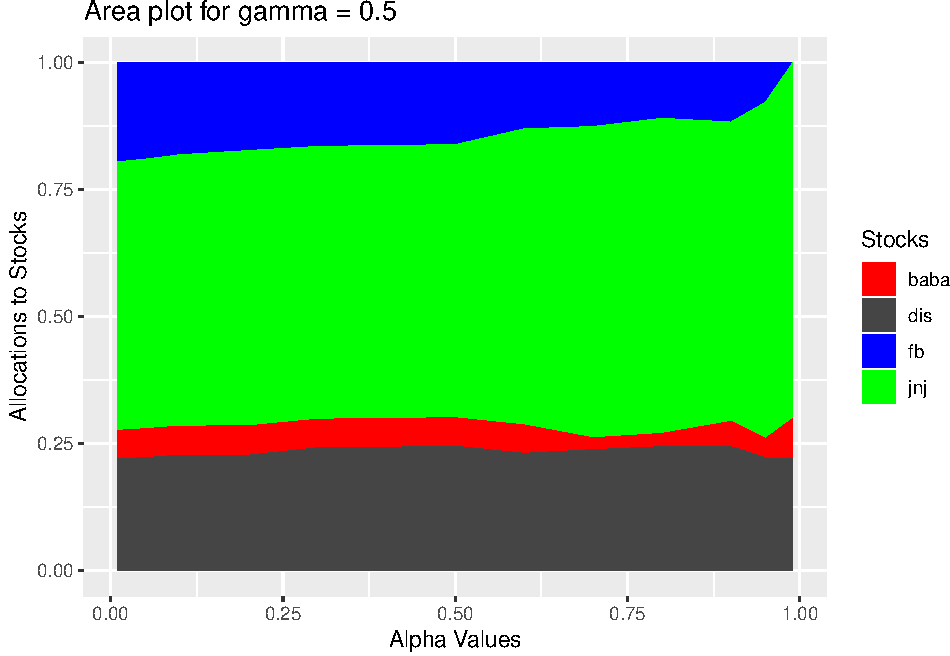
\includegraphics{Integrated_Management_Formulation_Model_files/figure-latex/unnamed-chunk-15-1.pdf}

\begin{Shaded}
\begin{Highlighting}[]
\NormalTok{data5 <-}\StringTok{ }\NormalTok{result5}
\KeywordTok{names}\NormalTok{(data5) <-}\StringTok{ }\KeywordTok{c}\NormalTok{(}\StringTok{"alpha"}\NormalTok{,}\StringTok{"DIS"}\NormalTok{,}\StringTok{"BABA"}\NormalTok{,}\StringTok{"JNJ"}\NormalTok{,}\StringTok{"FB"}\NormalTok{)}
\NormalTok{mdata5 <-}\StringTok{ }\KeywordTok{melt}\NormalTok{(data5, }\DataTypeTok{id=}\KeywordTok{c}\NormalTok{(}\StringTok{"alpha"}\NormalTok{))}
\KeywordTok{names}\NormalTok{(mdata5) <-}\StringTok{ }\KeywordTok{c}\NormalTok{(}\StringTok{"Alpha"}\NormalTok{,}\StringTok{"Stocks"}\NormalTok{,}\StringTok{"Allocation"}\NormalTok{)}
\KeywordTok{ggplot}\NormalTok{() }\OperatorTok{+}\StringTok{ }\KeywordTok{geom_bar}\NormalTok{(}\KeywordTok{aes}\NormalTok{(}\DataTypeTok{y =}\NormalTok{ Allocation, }\DataTypeTok{x =}\NormalTok{ Alpha, }\DataTypeTok{fill =}\NormalTok{ Stocks), }\DataTypeTok{data =}\NormalTok{ mdata5, }\DataTypeTok{stat=}\StringTok{"identity"}\NormalTok{)}\OperatorTok{+}
\StringTok{  }\KeywordTok{scale_fill_manual}\NormalTok{(}\StringTok{"Stocks"}\NormalTok{,}\DataTypeTok{values =}
                      \KeywordTok{c}\NormalTok{(}\StringTok{"FB"}\NormalTok{=}\StringTok{"#0000FF"}\NormalTok{,}\StringTok{"JNJ"}\NormalTok{=}\StringTok{"#00FF00"}\NormalTok{,}\StringTok{"BABA"}\NormalTok{=}\StringTok{"#FF0000"}\NormalTok{,}\StringTok{"DIS"}\NormalTok{=}\StringTok{"#454545"}\NormalTok{))}
\end{Highlighting}
\end{Shaded}

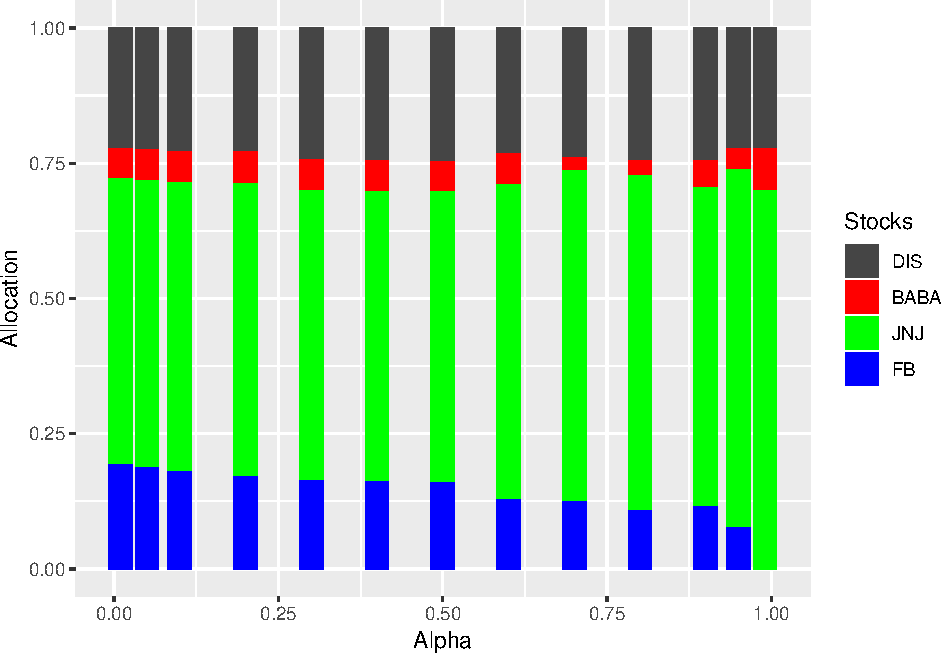
\includegraphics{Integrated_Management_Formulation_Model_files/figure-latex/unnamed-chunk-15-2.pdf}

\paragraph{Plot of alpha vs q for gamma =
0.5}\label{plot-of-alpha-vs-q-for-gamma-0.5}

\begin{Shaded}
\begin{Highlighting}[]
\NormalTok{result_q5 <-}\StringTok{ }\KeywordTok{data.frame}\NormalTok{(alpha,q_result5)}
\KeywordTok{write.csv}\NormalTok{(result_q5,}\DataTypeTok{file =} \StringTok{"VaR_Results5.csv"}\NormalTok{)}
\KeywordTok{ggplot}\NormalTok{(}\DataTypeTok{data=}\NormalTok{result_q5, }\KeywordTok{aes}\NormalTok{(}\DataTypeTok{x=}\NormalTok{alpha, }\DataTypeTok{y=}\NormalTok{q_result5, }\DataTypeTok{group=}\DecValTok{1}\NormalTok{)) }\OperatorTok{+}
\StringTok{  }\KeywordTok{geom_line}\NormalTok{(}\DataTypeTok{color=}\StringTok{"blue"}\NormalTok{)}\OperatorTok{+}
\StringTok{  }\KeywordTok{geom_point}\NormalTok{()}\OperatorTok{+}
\StringTok{  }\KeywordTok{labs}\NormalTok{(}\DataTypeTok{title=}\StringTok{"Plot of VaR vs Alpha for Gamma = 0.5 "}\NormalTok{,}\DataTypeTok{x=}\StringTok{"Value of Alpha"}\NormalTok{, }\DataTypeTok{y =} \StringTok{"Value At Risk"}\NormalTok{)}\OperatorTok{+}
\StringTok{  }\KeywordTok{theme_classic}\NormalTok{()}
\end{Highlighting}
\end{Shaded}

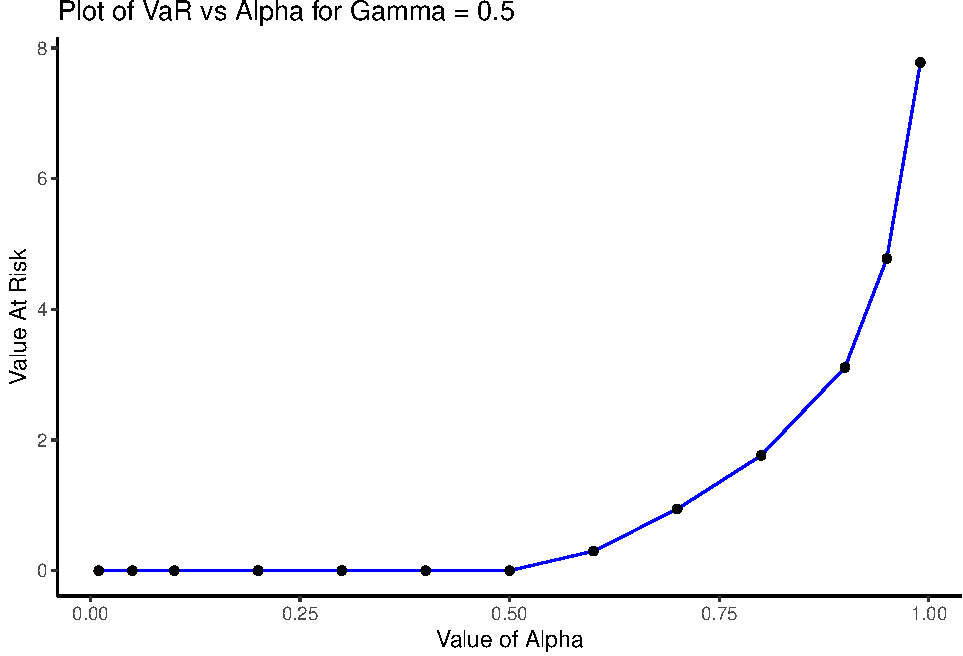
\includegraphics{Integrated_Management_Formulation_Model_files/figure-latex/unnamed-chunk-16-1.pdf}

\subsubsection{With gamma=0.7}\label{with-gamma0.7}

\begin{Shaded}
\begin{Highlighting}[]
\NormalTok{gamma7 =}\StringTok{ }\FloatTok{0.7}
\NormalTok{dis_result7 =}\StringTok{ }\KeywordTok{vector}\NormalTok{(}\DataTypeTok{mode =} \StringTok{"numeric"}\NormalTok{)}
\NormalTok{baba_result7 =}\StringTok{ }\KeywordTok{vector}\NormalTok{(}\DataTypeTok{mode =} \StringTok{"numeric"}\NormalTok{)}
\NormalTok{jnj_result7 =}\StringTok{ }\KeywordTok{vector}\NormalTok{(}\DataTypeTok{mode =} \StringTok{"numeric"}\NormalTok{)}
\NormalTok{fb_result7 =}\StringTok{ }\KeywordTok{vector}\NormalTok{(}\DataTypeTok{mode =} \StringTok{"numeric"}\NormalTok{)}
\NormalTok{q_result7 =}\StringTok{ }\KeywordTok{vector}\NormalTok{(}\DataTypeTok{mode =} \StringTok{"numeric"}\NormalTok{)}
\ControlFlowTok{for}\NormalTok{ (alp }\ControlFlowTok{in}\NormalTok{ alpha)\{}
\NormalTok{  objvect7 <-}\StringTok{ }\KeywordTok{c}\NormalTok{((}\DecValTok{1}\OperatorTok{-}\NormalTok{gamma7)}\OperatorTok{*}\KeywordTok{t}\NormalTok{(prob)}\OperatorTok\NormalTok{Portreturns,(}\OperatorTok{-}\NormalTok{gamma7}\OperatorTok{/}\NormalTok{(}\DecValTok{1}\OperatorTok{-}\NormalTok{alp))}\OperatorTok{*}\KeywordTok{t}\NormalTok{(prob),}\OperatorTok{-}\NormalTok{gamma7)}
  \KeywordTok{names}\NormalTok{(objvect7)<-}\KeywordTok{c}\NormalTok{(}\StringTok{"dis"}\NormalTok{,}\StringTok{"baba"}\NormalTok{,}\StringTok{"jnj"}\NormalTok{,}\StringTok{"fb"}\NormalTok{,}\KeywordTok{rep}\NormalTok{(}\StringTok{"z"}\NormalTok{,}\DecValTok{826}\NormalTok{),}\StringTok{"q"}\NormalTok{)}
\NormalTok{  Solution7 <-}\StringTok{ }\KeywordTok{solveLP}\NormalTok{(objvect7,rhscons,Amat,}\DataTypeTok{maximum =} \OtherTok{TRUE}\NormalTok{,}
          \DataTypeTok{const.dir =} \KeywordTok{c}\NormalTok{(}\KeywordTok{rep}\NormalTok{(}\StringTok{"<="}\NormalTok{,}\DecValTok{826}\NormalTok{),}\StringTok{"="}\NormalTok{,}\KeywordTok{rep}\NormalTok{(}\StringTok{"<="}\NormalTok{,}\DecValTok{830}\NormalTok{)),}\DataTypeTok{lpSolve =} \OtherTok{TRUE}\NormalTok{)}
\NormalTok{  dis_result7<-}\KeywordTok{append}\NormalTok{(dis_result7,Solution7}\OperatorTok{$}\NormalTok{solution[}\DecValTok{1}\NormalTok{])}
\NormalTok{  baba_result7<-}\KeywordTok{append}\NormalTok{(baba_result7,Solution7}\OperatorTok{$}\NormalTok{solution[}\DecValTok{2}\NormalTok{])}
\NormalTok{  jnj_result7<-}\KeywordTok{append}\NormalTok{(jnj_result7,Solution7}\OperatorTok{$}\NormalTok{solution[}\DecValTok{3}\NormalTok{])}
\NormalTok{  fb_result7<-}\KeywordTok{append}\NormalTok{(fb_result7,Solution7}\OperatorTok{$}\NormalTok{solution[}\DecValTok{4}\NormalTok{])}
\NormalTok{  q_result7 <-}\StringTok{ }\KeywordTok{append}\NormalTok{(q_result7,Solution7}\OperatorTok{$}\NormalTok{solution[}\DecValTok{831}\NormalTok{])}
\NormalTok{\}}
\end{Highlighting}
\end{Shaded}

\paragraph{\texorpdfstring{Asset allocation for
\(\gamma = 0.7\)}{Asset allocation for \textbackslash{}gamma = 0.7}}\label{asset-allocation-for-gamma-0.7}

\begin{Shaded}
\begin{Highlighting}[]
\NormalTok{result7 <-}\StringTok{  }\KeywordTok{data.frame}\NormalTok{(alpha,dis_result7,baba_result7,jnj_result7,fb_result7)}
\KeywordTok{write.csv}\NormalTok{(result7, }\DataTypeTok{file =} \StringTok{"Results7.csv"}\NormalTok{)}
\KeywordTok{ggplot}\NormalTok{(result7, }\KeywordTok{aes}\NormalTok{(}\DataTypeTok{x=}\NormalTok{result7}\OperatorTok{$}\NormalTok{alpha)) }\OperatorTok{+}\StringTok{ }
\StringTok{  }\KeywordTok{geom_area}\NormalTok{(}\KeywordTok{aes}\NormalTok{(}\DataTypeTok{y=}\NormalTok{result7}\OperatorTok{$}\NormalTok{dis_result7}\OperatorTok{+}\NormalTok{result7}\OperatorTok{$}\NormalTok{baba_result7}\OperatorTok{+}\NormalTok{result7}\OperatorTok{$}\NormalTok{jnj_result7}\OperatorTok{+}\NormalTok{result7}\OperatorTok{$}\NormalTok{fb_result7, }\DataTypeTok{fill=}\StringTok{"fb"}\NormalTok{))}\OperatorTok{+}
\StringTok{  }\KeywordTok{geom_area}\NormalTok{(}\KeywordTok{aes}\NormalTok{(}\DataTypeTok{y=}\NormalTok{result7}\OperatorTok{$}\NormalTok{dis_result7}\OperatorTok{+}\NormalTok{result7}\OperatorTok{$}\NormalTok{baba_result7}\OperatorTok{+}\NormalTok{result7}\OperatorTok{$}\NormalTok{jnj_result7, }\DataTypeTok{fill=}\StringTok{"jnj"}\NormalTok{)) }\OperatorTok{+}
\StringTok{  }\KeywordTok{geom_area}\NormalTok{(}\KeywordTok{aes}\NormalTok{(}\DataTypeTok{y=}\NormalTok{result7}\OperatorTok{$}\NormalTok{dis_result7}\OperatorTok{+}\NormalTok{result7}\OperatorTok{$}\NormalTok{baba_result7, }\DataTypeTok{fill=}\StringTok{"baba"}\NormalTok{)) }\OperatorTok{+}
\StringTok{  }\KeywordTok{geom_area}\NormalTok{(}\KeywordTok{aes}\NormalTok{(}\DataTypeTok{y=}\NormalTok{result7}\OperatorTok{$}\NormalTok{dis_result7,}\DataTypeTok{fill =} \StringTok{'dis'}\NormalTok{)) }\OperatorTok{+}\StringTok{ }
\StringTok{  }\KeywordTok{xlab}\NormalTok{(}\StringTok{"Alpha Values"}\NormalTok{) }\OperatorTok{+}\StringTok{ }\KeywordTok{ylab}\NormalTok{(}\StringTok{"Allocations to Stocks"}\NormalTok{) }\OperatorTok{+}
\StringTok{  }\KeywordTok{labs}\NormalTok{(}\DataTypeTok{title=}\StringTok{"Area plot for gamma = 0.7"}\NormalTok{) }\OperatorTok{+}
\StringTok{  }\KeywordTok{scale_fill_manual}\NormalTok{(}\StringTok{"Series"}\NormalTok{,}\DataTypeTok{values =} \KeywordTok{c}\NormalTok{(}\StringTok{"fb"}\NormalTok{=}\StringTok{"#0000FF"}\NormalTok{,}\StringTok{"jnj"}\NormalTok{=}\StringTok{"#00FF00"}\NormalTok{,}\StringTok{"baba"}\NormalTok{=}\StringTok{"#FF0000"}\NormalTok{,}\StringTok{"dis"}\NormalTok{=}\StringTok{"#454545"}\NormalTok{))}
\end{Highlighting}
\end{Shaded}

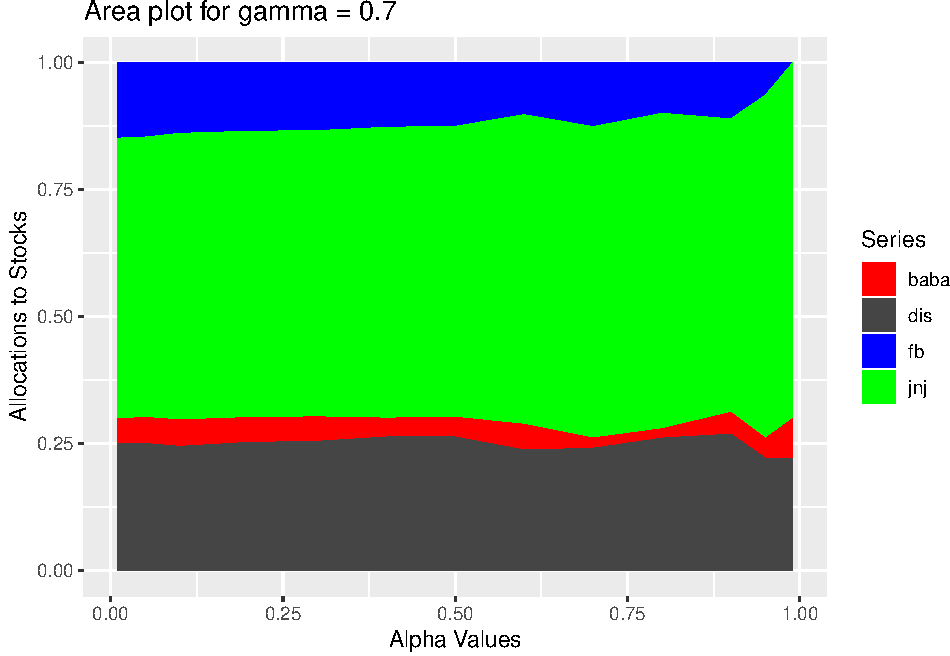
\includegraphics{Integrated_Management_Formulation_Model_files/figure-latex/unnamed-chunk-18-1.pdf}

\begin{Shaded}
\begin{Highlighting}[]
\NormalTok{data7 <-}\StringTok{ }\NormalTok{result7}
\KeywordTok{names}\NormalTok{(data7) <-}\StringTok{ }\KeywordTok{c}\NormalTok{(}\StringTok{"alpha"}\NormalTok{,}\StringTok{"DIS"}\NormalTok{,}\StringTok{"BABA"}\NormalTok{,}\StringTok{"JNJ"}\NormalTok{,}\StringTok{"FB"}\NormalTok{)}
\NormalTok{mdata7 <-}\StringTok{ }\KeywordTok{melt}\NormalTok{(data7, }\DataTypeTok{id=}\KeywordTok{c}\NormalTok{(}\StringTok{"alpha"}\NormalTok{))}
\KeywordTok{names}\NormalTok{(mdata7) <-}\StringTok{ }\KeywordTok{c}\NormalTok{(}\StringTok{"Alpha"}\NormalTok{,}\StringTok{"Stocks"}\NormalTok{,}\StringTok{"Allocation"}\NormalTok{)}
\KeywordTok{ggplot}\NormalTok{() }\OperatorTok{+}\StringTok{ }\KeywordTok{geom_bar}\NormalTok{(}\KeywordTok{aes}\NormalTok{(}\DataTypeTok{y =}\NormalTok{ Allocation, }\DataTypeTok{x =}\NormalTok{ Alpha, }\DataTypeTok{fill =}\NormalTok{ Stocks), }\DataTypeTok{data =}\NormalTok{ mdata7, }\DataTypeTok{stat=}\StringTok{"identity"}\NormalTok{)}\OperatorTok{+}
\StringTok{  }\KeywordTok{scale_fill_manual}\NormalTok{(}\StringTok{"Stocks"}\NormalTok{,}\DataTypeTok{values =}
                      \KeywordTok{c}\NormalTok{(}\StringTok{"FB"}\NormalTok{=}\StringTok{"#0000FF"}\NormalTok{,}\StringTok{"JNJ"}\NormalTok{=}\StringTok{"#00FF00"}\NormalTok{,}\StringTok{"BABA"}\NormalTok{=}\StringTok{"#FF0000"}\NormalTok{,}\StringTok{"DIS"}\NormalTok{=}\StringTok{"#454545"}\NormalTok{))}
\end{Highlighting}
\end{Shaded}

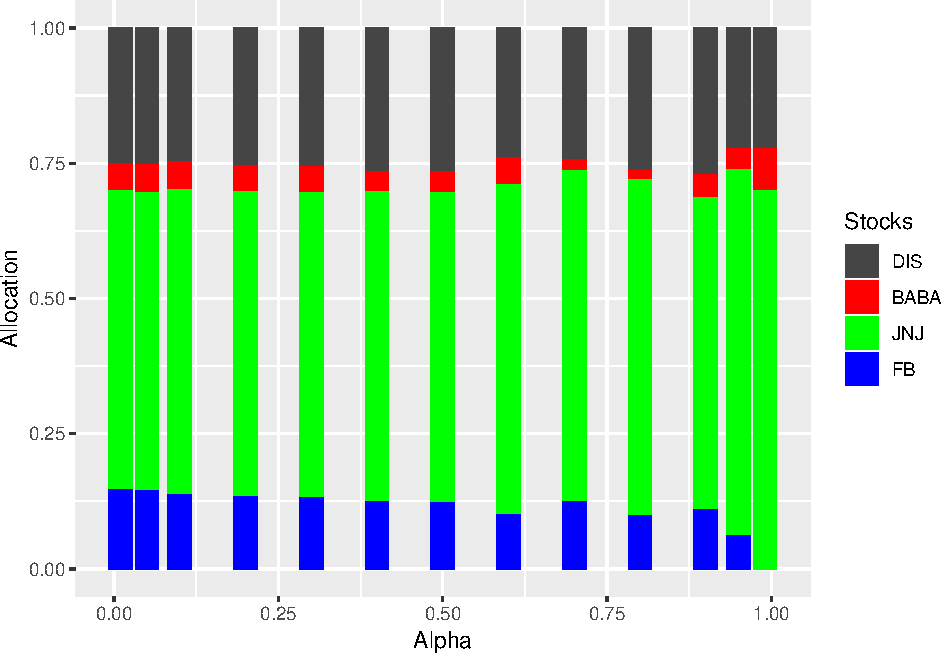
\includegraphics{Integrated_Management_Formulation_Model_files/figure-latex/unnamed-chunk-18-2.pdf}

\paragraph{Plot of alpha vs q for gamma =
0.7}\label{plot-of-alpha-vs-q-for-gamma-0.7}

\begin{Shaded}
\begin{Highlighting}[]
\NormalTok{result_q7 <-}\StringTok{ }\KeywordTok{data.frame}\NormalTok{(alpha,q_result7)}
\KeywordTok{write.csv}\NormalTok{(result_q7,}\DataTypeTok{file =} \StringTok{"VaR_Results7.csv"}\NormalTok{)}
\KeywordTok{ggplot}\NormalTok{(}\DataTypeTok{data=}\NormalTok{result_q7, }\KeywordTok{aes}\NormalTok{(}\DataTypeTok{x=}\NormalTok{alpha, }\DataTypeTok{y=}\NormalTok{q_result7, }\DataTypeTok{group=}\DecValTok{1}\NormalTok{)) }\OperatorTok{+}
\StringTok{  }\KeywordTok{geom_line}\NormalTok{(}\DataTypeTok{color=}\StringTok{"blue"}\NormalTok{)}\OperatorTok{+}
\StringTok{  }\KeywordTok{geom_point}\NormalTok{()}\OperatorTok{+}
\StringTok{  }\KeywordTok{labs}\NormalTok{(}\DataTypeTok{title=}\StringTok{"Plot of VaR vs Alpha for Gamma = 0.7 "}\NormalTok{,}\DataTypeTok{x=}\StringTok{"Value of Alpha"}\NormalTok{, }\DataTypeTok{y =} \StringTok{"Value At Risk"}\NormalTok{)}\OperatorTok{+}
\StringTok{  }\KeywordTok{theme_classic}\NormalTok{()}
\end{Highlighting}
\end{Shaded}

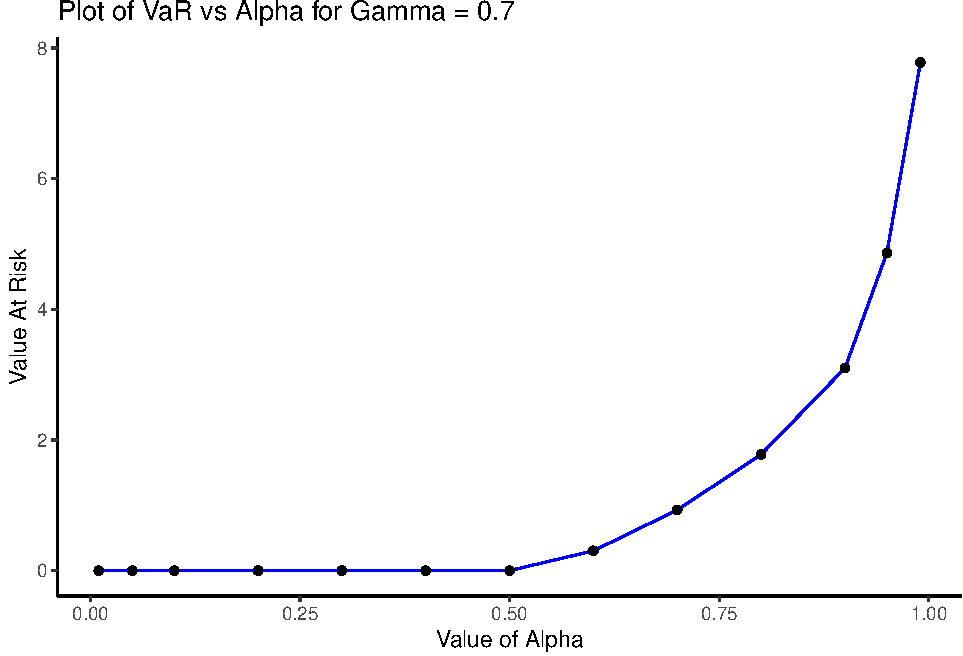
\includegraphics{Integrated_Management_Formulation_Model_files/figure-latex/unnamed-chunk-19-1.pdf}

\subsubsection{With gamma=0.9}\label{with-gamma0.9}

\begin{Shaded}
\begin{Highlighting}[]
\NormalTok{gamma9 =}\StringTok{ }\FloatTok{0.9}
\NormalTok{dis_result9 =}\StringTok{ }\KeywordTok{vector}\NormalTok{(}\DataTypeTok{mode =} \StringTok{"numeric"}\NormalTok{)}
\NormalTok{baba_result9 =}\StringTok{ }\KeywordTok{vector}\NormalTok{(}\DataTypeTok{mode =} \StringTok{"numeric"}\NormalTok{)}
\NormalTok{jnj_result9 =}\StringTok{ }\KeywordTok{vector}\NormalTok{(}\DataTypeTok{mode =} \StringTok{"numeric"}\NormalTok{)}
\NormalTok{fb_result9 =}\StringTok{ }\KeywordTok{vector}\NormalTok{(}\DataTypeTok{mode =} \StringTok{"numeric"}\NormalTok{)}
\NormalTok{q_result9 =}\StringTok{ }\KeywordTok{vector}\NormalTok{(}\DataTypeTok{mode =} \StringTok{"numeric"}\NormalTok{)}
\ControlFlowTok{for}\NormalTok{ (alp }\ControlFlowTok{in}\NormalTok{ alpha)\{}
\NormalTok{  objvect9 <-}\StringTok{ }\KeywordTok{c}\NormalTok{((}\DecValTok{1}\OperatorTok{-}\NormalTok{gamma9)}\OperatorTok{*}\KeywordTok{t}\NormalTok{(prob)}\OperatorTok\NormalTok{Portreturns,(}\OperatorTok{-}\NormalTok{gamma9}\OperatorTok{/}\NormalTok{(}\DecValTok{1}\OperatorTok{-}\NormalTok{alp))}\OperatorTok{*}\KeywordTok{t}\NormalTok{(prob),}\OperatorTok{-}\NormalTok{gamma9)}
  \KeywordTok{names}\NormalTok{(objvect9)<-}\KeywordTok{c}\NormalTok{(}\StringTok{"dis"}\NormalTok{,}\StringTok{"baba"}\NormalTok{,}\StringTok{"jnj"}\NormalTok{,}\StringTok{"fb"}\NormalTok{,}\KeywordTok{rep}\NormalTok{(}\StringTok{"z"}\NormalTok{,}\DecValTok{826}\NormalTok{),}\StringTok{"q"}\NormalTok{)}
\NormalTok{  Solution9 <-}\StringTok{ }\KeywordTok{solveLP}\NormalTok{(objvect9,rhscons,Amat,}\DataTypeTok{maximum =} \OtherTok{TRUE}\NormalTok{,}
          \DataTypeTok{const.dir =} \KeywordTok{c}\NormalTok{(}\KeywordTok{rep}\NormalTok{(}\StringTok{"<="}\NormalTok{,}\DecValTok{826}\NormalTok{),}\StringTok{"="}\NormalTok{,}\KeywordTok{rep}\NormalTok{(}\StringTok{"<="}\NormalTok{,}\DecValTok{830}\NormalTok{)),}\DataTypeTok{lpSolve =} \OtherTok{TRUE}\NormalTok{)}
\NormalTok{  dis_result9<-}\KeywordTok{append}\NormalTok{(dis_result9,Solution9}\OperatorTok{$}\NormalTok{solution[}\DecValTok{1}\NormalTok{])}
\NormalTok{  baba_result9<-}\KeywordTok{append}\NormalTok{(baba_result9,Solution9}\OperatorTok{$}\NormalTok{solution[}\DecValTok{2}\NormalTok{])}
\NormalTok{  jnj_result9<-}\KeywordTok{append}\NormalTok{(jnj_result9,Solution9}\OperatorTok{$}\NormalTok{solution[}\DecValTok{3}\NormalTok{])}
\NormalTok{  fb_result9<-}\KeywordTok{append}\NormalTok{(fb_result9,Solution9}\OperatorTok{$}\NormalTok{solution[}\DecValTok{4}\NormalTok{])}
\NormalTok{  q_result9 <-}\StringTok{ }\KeywordTok{append}\NormalTok{(q_result9,Solution9}\OperatorTok{$}\NormalTok{solution[}\DecValTok{831}\NormalTok{])}
\NormalTok{\}}
\end{Highlighting}
\end{Shaded}

\paragraph{\texorpdfstring{Asset allocation for
\(\gamma=0.9\)}{Asset allocation for \textbackslash{}gamma=0.9}}\label{asset-allocation-for-gamma0.9}

\begin{Shaded}
\begin{Highlighting}[]
\NormalTok{result9 <-}\StringTok{  }\KeywordTok{data.frame}\NormalTok{(alpha,dis_result9,baba_result9,jnj_result9,fb_result9)}
\KeywordTok{write.csv}\NormalTok{(result9, }\DataTypeTok{file =} \StringTok{"Results9.csv"}\NormalTok{)}
\KeywordTok{ggplot}\NormalTok{(result9, }\KeywordTok{aes}\NormalTok{(}\DataTypeTok{x=}\NormalTok{result9}\OperatorTok{$}\NormalTok{alpha)) }\OperatorTok{+}\StringTok{ }
\StringTok{  }\KeywordTok{geom_area}\NormalTok{(}\KeywordTok{aes}\NormalTok{(}\DataTypeTok{y=}\NormalTok{result9}\OperatorTok{$}\NormalTok{dis_result9}\OperatorTok{+}\NormalTok{result9}\OperatorTok{$}\NormalTok{baba_result9}\OperatorTok{+}\NormalTok{result9}\OperatorTok{$}\NormalTok{jnj_result9}\OperatorTok{+}\NormalTok{result9}\OperatorTok{$}\NormalTok{fb_result9, }\DataTypeTok{fill=}\StringTok{"fb"}\NormalTok{))}\OperatorTok{+}
\StringTok{  }\KeywordTok{geom_area}\NormalTok{(}\KeywordTok{aes}\NormalTok{(}\DataTypeTok{y=}\NormalTok{result9}\OperatorTok{$}\NormalTok{dis_result9}\OperatorTok{+}\NormalTok{result9}\OperatorTok{$}\NormalTok{baba_result9}\OperatorTok{+}\NormalTok{result9}\OperatorTok{$}\NormalTok{jnj_result9, }\DataTypeTok{fill=}\StringTok{"jnj"}\NormalTok{)) }\OperatorTok{+}
\StringTok{  }\KeywordTok{geom_area}\NormalTok{(}\KeywordTok{aes}\NormalTok{(}\DataTypeTok{y=}\NormalTok{result9}\OperatorTok{$}\NormalTok{dis_result9}\OperatorTok{+}\NormalTok{result9}\OperatorTok{$}\NormalTok{baba_result9, }\DataTypeTok{fill=}\StringTok{"baba"}\NormalTok{)) }\OperatorTok{+}
\StringTok{  }\KeywordTok{geom_area}\NormalTok{(}\KeywordTok{aes}\NormalTok{(}\DataTypeTok{y=}\NormalTok{result9}\OperatorTok{$}\NormalTok{dis_result9,}\DataTypeTok{fill =} \StringTok{'dis'}\NormalTok{)) }\OperatorTok{+}\StringTok{ }
\StringTok{  }\KeywordTok{xlab}\NormalTok{(}\StringTok{"Alpha Values"}\NormalTok{) }\OperatorTok{+}\StringTok{ }\KeywordTok{ylab}\NormalTok{(}\StringTok{"Allocations to Stocks"}\NormalTok{) }\OperatorTok{+}
\StringTok{  }\KeywordTok{labs}\NormalTok{(}\DataTypeTok{title=}\StringTok{"Area plot for gamma = 0.9"}\NormalTok{)}\OperatorTok{+}
\StringTok{  }\KeywordTok{scale_fill_manual}\NormalTok{(}\StringTok{"Stocks"}\NormalTok{,}\DataTypeTok{values =} \KeywordTok{c}\NormalTok{(}\StringTok{"fb"}\NormalTok{=}\StringTok{"#0000FF"}\NormalTok{,}\StringTok{"jnj"}\NormalTok{=}\StringTok{"#00FF00"}\NormalTok{,}\StringTok{"baba"}\NormalTok{=}\StringTok{"#FF0000"}\NormalTok{,}\StringTok{"dis"}\NormalTok{=}\StringTok{"#454545"}\NormalTok{))}
\end{Highlighting}
\end{Shaded}

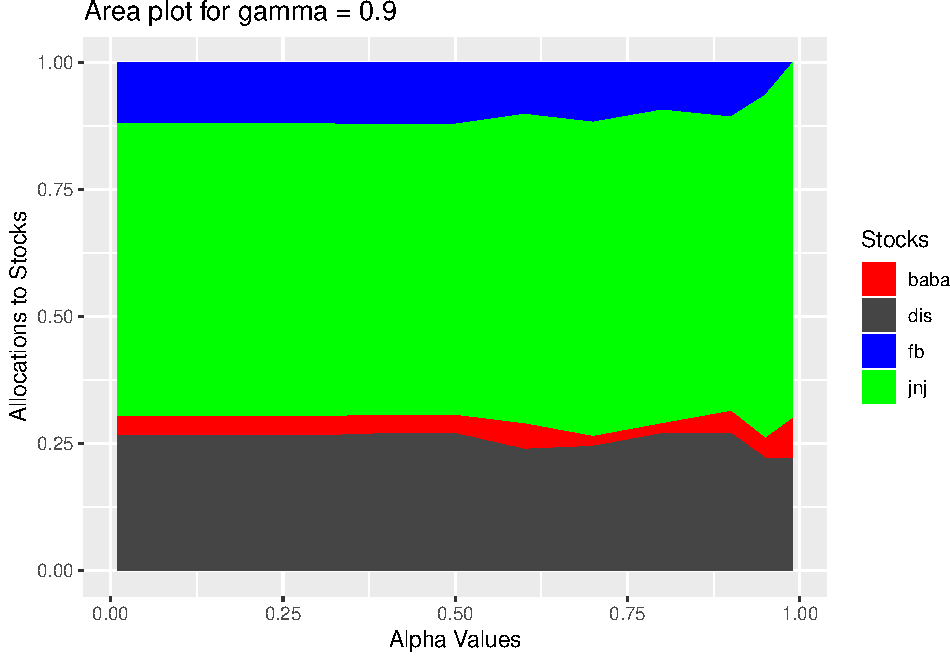
\includegraphics{Integrated_Management_Formulation_Model_files/figure-latex/unnamed-chunk-21-1.pdf}

\begin{Shaded}
\begin{Highlighting}[]
\NormalTok{data9 <-}\StringTok{ }\NormalTok{result9}
\KeywordTok{names}\NormalTok{(data9) <-}\StringTok{ }\KeywordTok{c}\NormalTok{(}\StringTok{"alpha"}\NormalTok{,}\StringTok{"DIS"}\NormalTok{,}\StringTok{"BABA"}\NormalTok{,}\StringTok{"JNJ"}\NormalTok{,}\StringTok{"FB"}\NormalTok{)}
\NormalTok{mdata9 <-}\StringTok{ }\KeywordTok{melt}\NormalTok{(data9, }\DataTypeTok{id=}\KeywordTok{c}\NormalTok{(}\StringTok{"alpha"}\NormalTok{))}
\KeywordTok{names}\NormalTok{(mdata9) <-}\StringTok{ }\KeywordTok{c}\NormalTok{(}\StringTok{"Alpha"}\NormalTok{,}\StringTok{"Stocks"}\NormalTok{,}\StringTok{"Allocation"}\NormalTok{)}
\KeywordTok{ggplot}\NormalTok{() }\OperatorTok{+}\StringTok{ }\KeywordTok{geom_bar}\NormalTok{(}\KeywordTok{aes}\NormalTok{(}\DataTypeTok{y =}\NormalTok{ Allocation, }\DataTypeTok{x =}\NormalTok{ Alpha, }\DataTypeTok{fill =}\NormalTok{ Stocks), }\DataTypeTok{data =}\NormalTok{ mdata9, }\DataTypeTok{stat=}\StringTok{"identity"}\NormalTok{)}\OperatorTok{+}
\StringTok{  }\KeywordTok{scale_fill_manual}\NormalTok{(}\StringTok{"Stocks"}\NormalTok{,}\DataTypeTok{values =}
                      \KeywordTok{c}\NormalTok{(}\StringTok{"FB"}\NormalTok{=}\StringTok{"#0000FF"}\NormalTok{,}\StringTok{"JNJ"}\NormalTok{=}\StringTok{"#00FF00"}\NormalTok{,}\StringTok{"BABA"}\NormalTok{=}\StringTok{"#FF0000"}\NormalTok{,}\StringTok{"DIS"}\NormalTok{=}\StringTok{"#454545"}\NormalTok{))}
\end{Highlighting}
\end{Shaded}

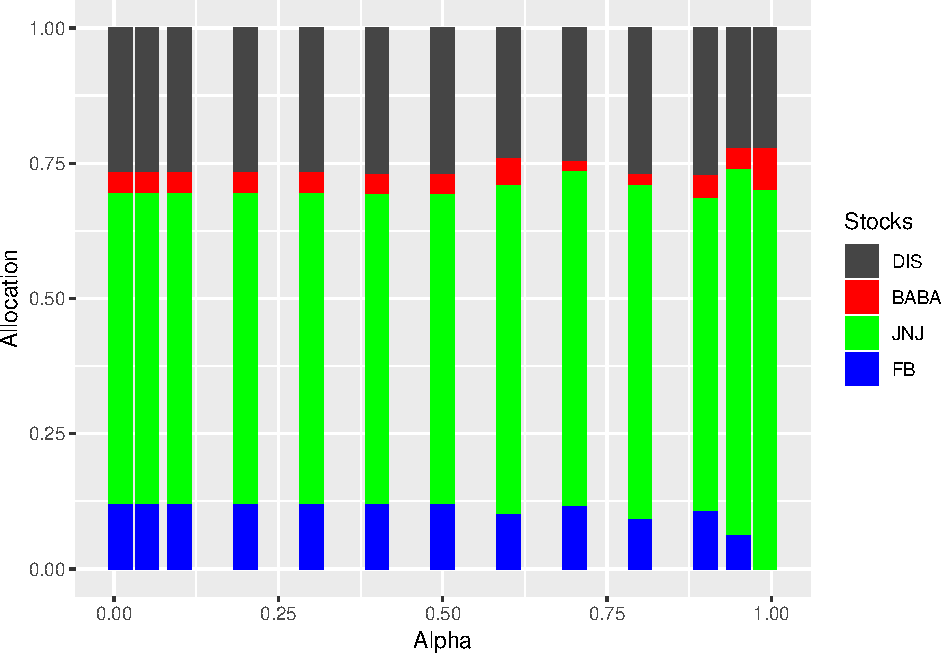
\includegraphics{Integrated_Management_Formulation_Model_files/figure-latex/unnamed-chunk-21-2.pdf}

\paragraph{Plot of alpha vs q(value at risk) for gamma =
0.9}\label{plot-of-alpha-vs-qvalue-at-risk-for-gamma-0.9}

\begin{Shaded}
\begin{Highlighting}[]
\NormalTok{result_q9 <-}\StringTok{ }\KeywordTok{data.frame}\NormalTok{(alpha,q_result9)}
\KeywordTok{write.csv}\NormalTok{(result_q9,}\DataTypeTok{file =} \StringTok{"VaR_Results9.csv"}\NormalTok{)}
\KeywordTok{ggplot}\NormalTok{(}\DataTypeTok{data=}\NormalTok{result_q9, }\KeywordTok{aes}\NormalTok{(}\DataTypeTok{x=}\NormalTok{alpha, }\DataTypeTok{y=}\NormalTok{q_result9, }\DataTypeTok{group=}\DecValTok{1}\NormalTok{)) }\OperatorTok{+}
\StringTok{  }\KeywordTok{geom_line}\NormalTok{(}\DataTypeTok{color=}\StringTok{"blue"}\NormalTok{)}\OperatorTok{+}
\StringTok{  }\KeywordTok{geom_point}\NormalTok{()}\OperatorTok{+}
\StringTok{  }\KeywordTok{labs}\NormalTok{(}\DataTypeTok{title=}\StringTok{"Plot of VaR vs Alpha for Gamma = 0.9"}\NormalTok{,}\DataTypeTok{x=}\StringTok{"Value of Alpha"}\NormalTok{, }\DataTypeTok{y =} \StringTok{"Value At Risk"}\NormalTok{)}\OperatorTok{+}
\StringTok{  }\KeywordTok{theme_classic}\NormalTok{()}
\end{Highlighting}
\end{Shaded}

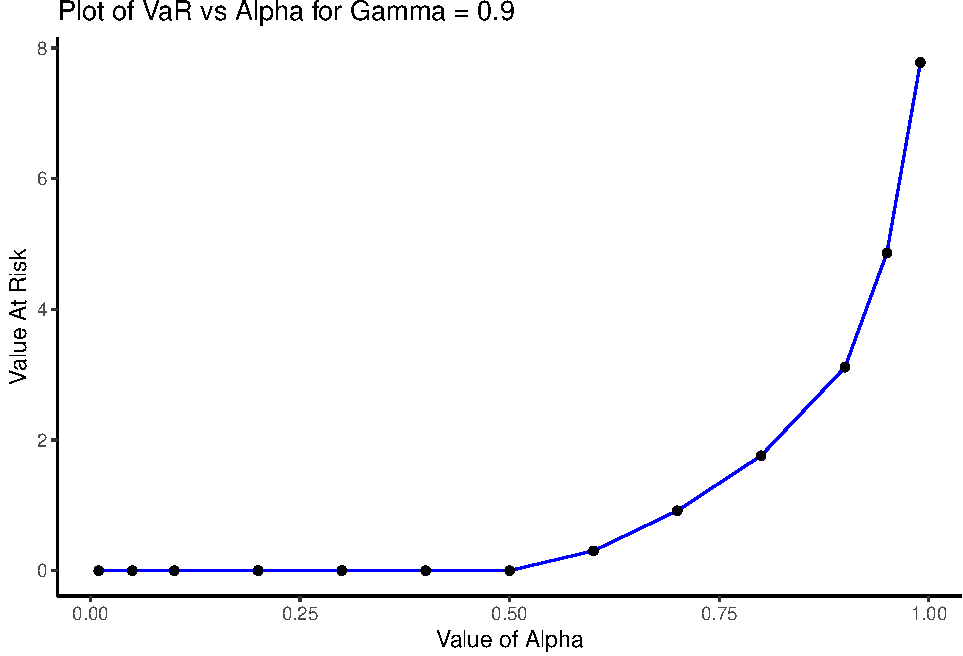
\includegraphics{Integrated_Management_Formulation_Model_files/figure-latex/unnamed-chunk-22-1.pdf}

\section{OPTIMIZATION WITH A RISK-LESS ASSET
ADDED}\label{optimization-with-a-risk-less-asset-added}

Having added a risk less asset(BOND), we will have a total of 5 assets
in our portfolio. The main problem is to show what ahhpens when a risk
less asset is included in the portfolio. The main result for this model
is that, for higher levels of \(\gamma\), the risk less asset becomes
more and more important i.e, the risk less asset gets more and more
weights as the level of \(\gamma\) increases.

\subsection{\texorpdfstring{Solving and asset allocation for
\(\gamma = 0.1\)}{Solving and asset allocation for \textbackslash{}gamma = 0.1}}\label{solving-and-asset-allocation-for-gamma-0.1}

The same way as in the solution of the model with only risky assets, the
\textbf{Amatfree} matrix doesn't change and therefore once created, we
will use the same matrix for all levels of \(\gamma\) that we are
considering.

\begin{Shaded}
\begin{Highlighting}[]
\NormalTok{gammafree1 =}\StringTok{ }\FloatTok{0.1}
\NormalTok{dis_resultfree1 =}\StringTok{ }\KeywordTok{vector}\NormalTok{(}\DataTypeTok{mode =} \StringTok{"numeric"}\NormalTok{)}
\NormalTok{baba_resultfree1 =}\StringTok{ }\KeywordTok{vector}\NormalTok{(}\DataTypeTok{mode =} \StringTok{"numeric"}\NormalTok{)}
\NormalTok{jnj_resultfree1 =}\StringTok{ }\KeywordTok{vector}\NormalTok{(}\DataTypeTok{mode =} \StringTok{"numeric"}\NormalTok{)}
\NormalTok{fb_resultfree1 =}\StringTok{ }\KeywordTok{vector}\NormalTok{(}\DataTypeTok{mode =} \StringTok{"numeric"}\NormalTok{)}
\NormalTok{bond_resultfree1 =}\StringTok{ }\KeywordTok{vector}\NormalTok{(}\DataTypeTok{mode =} \StringTok{"numeric"}\NormalTok{)}
\ControlFlowTok{for}\NormalTok{ (alp }\ControlFlowTok{in}\NormalTok{ alpha)\{}
\NormalTok{  objvectfree1 <-}\StringTok{ }\KeywordTok{c}\NormalTok{((}\DecValTok{1}\OperatorTok{-}\NormalTok{gammafree1)}\OperatorTok{*}\KeywordTok{t}\NormalTok{(prob)}\OperatorTok\NormalTok{Portreturnsfree,(}\OperatorTok{-}\NormalTok{gammafree1}\OperatorTok{/}\NormalTok{(}\DecValTok{1}\OperatorTok{-}\NormalTok{alp))}\OperatorTok{*}\KeywordTok{t}\NormalTok{(prob),}\OperatorTok{-}\NormalTok{gammafree1)}
  \KeywordTok{names}\NormalTok{(objvectfree1)<-}\KeywordTok{c}\NormalTok{(}\StringTok{"dis"}\NormalTok{,}\StringTok{"baba"}\NormalTok{,}\StringTok{"jnj"}\NormalTok{,}\StringTok{"fb"}\NormalTok{,}\StringTok{"bond"}\NormalTok{,}\KeywordTok{rep}\NormalTok{(}\StringTok{"z"}\NormalTok{,}\DecValTok{826}\NormalTok{),}\StringTok{"q"}\NormalTok{) }
\NormalTok{  rhsconsfree1 <-}\StringTok{ }\KeywordTok{c}\NormalTok{(}\KeywordTok{rep}\NormalTok{(}\DecValTok{0}\NormalTok{,}\DecValTok{826}\NormalTok{ ),}\DecValTok{1}\NormalTok{,}\KeywordTok{rep}\NormalTok{(}\DecValTok{0}\NormalTok{,}\DecValTok{831}\NormalTok{))}
\CommentTok{#Construction of matrix Amat}
\NormalTok{  firstconsfree =}\StringTok{ }\KeywordTok{cbind}\NormalTok{(}\OperatorTok{-}\NormalTok{Portreturnsfree,}\OperatorTok{-}\KeywordTok{diag}\NormalTok{(}\DecValTok{826}\NormalTok{),}\OperatorTok{-}\KeywordTok{rep}\NormalTok{(}\DecValTok{1}\NormalTok{,}\DecValTok{826}\NormalTok{))}
\NormalTok{  secondconsfree =}\StringTok{ }\NormalTok{(}\KeywordTok{c}\NormalTok{(}\KeywordTok{rep}\NormalTok{(}\DecValTok{1}\NormalTok{,}\DecValTok{5}\NormalTok{),}\KeywordTok{rep}\NormalTok{(}\DecValTok{0}\NormalTok{,}\DecValTok{827}\NormalTok{)))}
\NormalTok{  lessxfree =}\StringTok{ }\KeywordTok{cbind}\NormalTok{(}\OperatorTok{-}\KeywordTok{diag}\NormalTok{(}\DecValTok{5}\NormalTok{),}\KeywordTok{zeros}\NormalTok{(}\DecValTok{5}\NormalTok{,}\DecValTok{827}\NormalTok{))}
\NormalTok{  lesszfree =}\StringTok{ }\KeywordTok{cbind}\NormalTok{(}\KeywordTok{zeros}\NormalTok{(}\DecValTok{826}\NormalTok{,}\DecValTok{5}\NormalTok{),}\OperatorTok{-}\KeywordTok{diag}\NormalTok{(}\DecValTok{826}\NormalTok{),}\KeywordTok{rep}\NormalTok{(}\DecValTok{0}\NormalTok{,}\DecValTok{826}\NormalTok{))}
\NormalTok{  Amatfree =}\StringTok{ }\KeywordTok{rbind}\NormalTok{(firstconsfree,secondconsfree,lessxfree,lesszfree)}
  \KeywordTok{dim}\NormalTok{(Amatfree)}
  \KeywordTok{colnames}\NormalTok{(Amatfree) =}\StringTok{ }\OtherTok{NULL}
  \KeywordTok{rownames}\NormalTok{(Amatfree) =}\StringTok{ }\OtherTok{NULL}
\CommentTok{#solution of the problem using linprog}
\NormalTok{  Solutionfree1 <-}\StringTok{ }\KeywordTok{solveLP}\NormalTok{(objvectfree1,rhsconsfree1,Amatfree,}\DataTypeTok{maximum =} \OtherTok{TRUE}\NormalTok{,}
          \DataTypeTok{const.dir =} \KeywordTok{c}\NormalTok{(}\KeywordTok{rep}\NormalTok{(}\StringTok{"<="}\NormalTok{,}\DecValTok{826}\NormalTok{),}\StringTok{"="}\NormalTok{,}\KeywordTok{rep}\NormalTok{(}\StringTok{"<="}\NormalTok{,}\DecValTok{831}\NormalTok{)),}\DataTypeTok{lpSolve =} \OtherTok{TRUE}\NormalTok{)}
\NormalTok{  dis_resultfree1<-}\KeywordTok{append}\NormalTok{(dis_resultfree1,Solutionfree1}\OperatorTok{$}\NormalTok{solution[}\DecValTok{1}\NormalTok{])}
\NormalTok{  baba_resultfree1<-}\StringTok{ }\KeywordTok{append}\NormalTok{(baba_resultfree1,Solutionfree1}\OperatorTok{$}\NormalTok{solution[}\DecValTok{2}\NormalTok{])}
\NormalTok{  jnj_resultfree1<-}\KeywordTok{append}\NormalTok{(jnj_resultfree1,Solutionfree1}\OperatorTok{$}\NormalTok{solution[}\DecValTok{3}\NormalTok{])}
\NormalTok{  fb_resultfree1<-}\KeywordTok{append}\NormalTok{(fb_resultfree1,Solutionfree1}\OperatorTok{$}\NormalTok{solution[}\DecValTok{4}\NormalTok{])}
\NormalTok{  bond_resultfree1<-}\KeywordTok{append}\NormalTok{(bond_resultfree1,Solutionfree1}\OperatorTok{$}\NormalTok{solution[}\DecValTok{5}\NormalTok{])}
\NormalTok{\}}
\NormalTok{  resultfree1 <-}\KeywordTok{data.frame}\NormalTok{(alpha,dis_resultfree1,baba_resultfree1,jnj_resultfree1,}
\NormalTok{                           fb_resultfree1,bond_resultfree1)}
  \KeywordTok{write.csv}\NormalTok{(resultfree1, }\DataTypeTok{file =} \StringTok{"Resultsfree01.csv"}\NormalTok{)}
  \KeywordTok{ggplot}\NormalTok{(resultfree1, }\KeywordTok{aes}\NormalTok{(}\DataTypeTok{x=}\NormalTok{resultfree1}\OperatorTok{$}\NormalTok{alpha)) }\OperatorTok{+}\StringTok{ }
\StringTok{    }\KeywordTok{geom_area}\NormalTok{(}\KeywordTok{aes}\NormalTok{(}\DataTypeTok{y=}\NormalTok{resultfree1}\OperatorTok{$}\NormalTok{dis_resultfree1}\OperatorTok{+}\NormalTok{resultfree1}\OperatorTok{$}\NormalTok{baba_resultfree1}\OperatorTok{+}
\StringTok{                    }\NormalTok{resultfree1}\OperatorTok{$}\NormalTok{jnj_resultfree1}\OperatorTok{+}\NormalTok{resultfree1}\OperatorTok{$}\NormalTok{fb_resultfree1}\OperatorTok{+}
\StringTok{                    }\NormalTok{resultfree1}\OperatorTok{$}\NormalTok{bond_resultfree1, }\DataTypeTok{fill=}\StringTok{"bond"}\NormalTok{))}\OperatorTok{+}
\StringTok{    }\KeywordTok{geom_area}\NormalTok{(}\KeywordTok{aes}\NormalTok{(}\DataTypeTok{y=}\NormalTok{resultfree1}\OperatorTok{$}\NormalTok{dis_resultfree1}\OperatorTok{+}\NormalTok{resultfree1}\OperatorTok{$}\NormalTok{baba_resultfree1}\OperatorTok{+}
\StringTok{                    }\NormalTok{resultfree1}\OperatorTok{$}\NormalTok{jnj_resultfree1}\OperatorTok{+}\NormalTok{resultfree1}\OperatorTok{$}\NormalTok{fb_resultfree1, }\DataTypeTok{fill=}\StringTok{"fb"}\NormalTok{)) }\OperatorTok{+}
\StringTok{    }\KeywordTok{geom_area}\NormalTok{(}\KeywordTok{aes}\NormalTok{(}\DataTypeTok{y=}\NormalTok{resultfree1}\OperatorTok{$}\NormalTok{dis_resultfree1}\OperatorTok{+}\NormalTok{resultfree1}\OperatorTok{$}\NormalTok{baba_resultfree1}\OperatorTok{+}
\StringTok{                    }\NormalTok{resultfree1}\OperatorTok{$}\NormalTok{jnj_resultfree1, }\DataTypeTok{fill=}\StringTok{"jnj"}\NormalTok{)) }\OperatorTok{+}
\StringTok{    }\KeywordTok{geom_area}\NormalTok{(}\KeywordTok{aes}\NormalTok{(}\DataTypeTok{y=}\NormalTok{resultfree1}\OperatorTok{$}\NormalTok{dis_resultfree1}\OperatorTok{+}\NormalTok{resultfree1}\OperatorTok{$}\NormalTok{baba_resultfree1,}\DataTypeTok{fill =} \StringTok{'baba'}\NormalTok{)) }\OperatorTok{+}
\StringTok{    }\KeywordTok{geom_area}\NormalTok{(}\KeywordTok{aes}\NormalTok{(}\DataTypeTok{y=}\NormalTok{resultfree1}\OperatorTok{$}\NormalTok{dis_resultfree1,}\DataTypeTok{fill =} \StringTok{"dis"}\NormalTok{))}\OperatorTok{+}
\StringTok{    }\KeywordTok{xlab}\NormalTok{(}\StringTok{"alpha levels"}\NormalTok{) }\OperatorTok{+}\StringTok{ }\KeywordTok{ylab}\NormalTok{(}\StringTok{"Weights on the stocks"}\NormalTok{) }\OperatorTok{+}
\StringTok{    }\KeywordTok{labs}\NormalTok{(}\DataTypeTok{title=}\StringTok{"Asset allocation for gamma = 0.1"}\NormalTok{) }\OperatorTok{+}\StringTok{  }\CommentTok{# title and caption}
\StringTok{    }\KeywordTok{scale_fill_manual}\NormalTok{(}\StringTok{"Stocks"}\NormalTok{,}
                      \DataTypeTok{values =}\KeywordTok{c}\NormalTok{(}\StringTok{"fb"}\NormalTok{=}\StringTok{"#0000FF"}\NormalTok{,}\StringTok{"jnj"}\NormalTok{=}\StringTok{"#00FF00"}\NormalTok{,}\StringTok{"baba"}\NormalTok{=}\StringTok{"#FF0000"}\NormalTok{,}\StringTok{"dis"}\NormalTok{=}\StringTok{"#454545"}\NormalTok{,}\StringTok{"bond"}\NormalTok{=}\StringTok{"violet"}\NormalTok{))}
\end{Highlighting}
\end{Shaded}

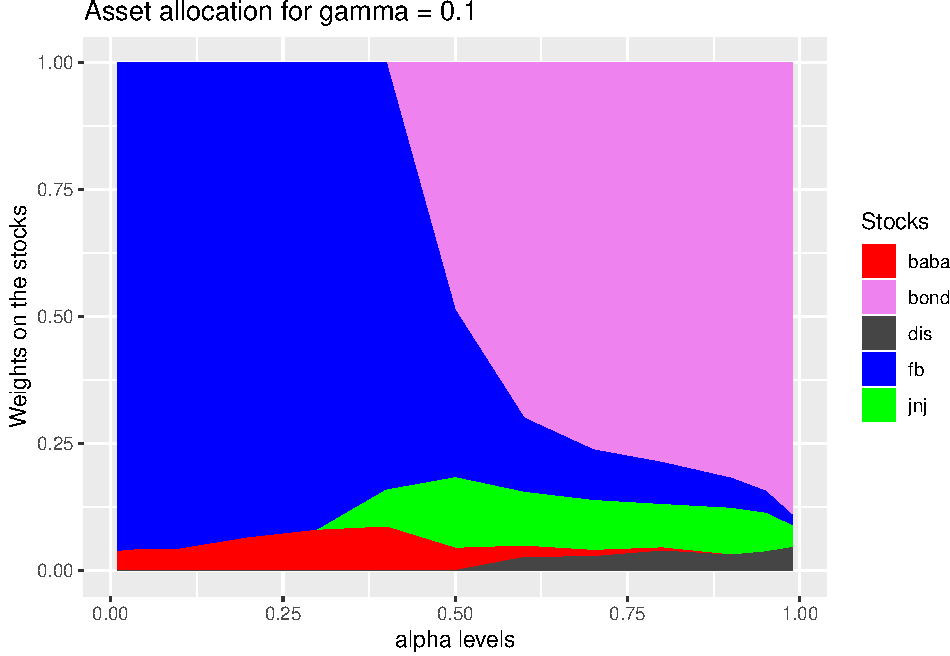
\includegraphics{Integrated_Management_Formulation_Model_files/figure-latex/unnamed-chunk-23-1.pdf}

\begin{Shaded}
\begin{Highlighting}[]
\CommentTok{# Using stacked barplots }
\KeywordTok{library}\NormalTok{(reshape2)}
\NormalTok{data1 <-}\StringTok{ }\NormalTok{resultfree1}
\KeywordTok{names}\NormalTok{(data1) <-}\StringTok{ }\KeywordTok{c}\NormalTok{(}\StringTok{"alpha"}\NormalTok{,}\StringTok{"DIS"}\NormalTok{,}\StringTok{"BABA"}\NormalTok{,}\StringTok{"JNJ"}\NormalTok{,}\StringTok{"FB"}\NormalTok{,}\StringTok{"BOND"}\NormalTok{)}
\NormalTok{mdata1 <-}\StringTok{ }\KeywordTok{melt}\NormalTok{(data1, }\DataTypeTok{id=}\KeywordTok{c}\NormalTok{(}\StringTok{"alpha"}\NormalTok{))}
\KeywordTok{names}\NormalTok{(mdata1) <-}\StringTok{ }\KeywordTok{c}\NormalTok{(}\StringTok{"Alpha"}\NormalTok{,}\StringTok{"Stocks"}\NormalTok{,}\StringTok{"Allocation"}\NormalTok{)}
\KeywordTok{ggplot}\NormalTok{() }\OperatorTok{+}\StringTok{ }\KeywordTok{geom_bar}\NormalTok{(}\KeywordTok{aes}\NormalTok{(}\DataTypeTok{y =}\NormalTok{ Allocation, }\DataTypeTok{x =}\NormalTok{ Alpha, }\DataTypeTok{fill =}\NormalTok{ Stocks), }\DataTypeTok{data =}\NormalTok{ mdata1, }\DataTypeTok{stat=}\StringTok{"identity"}\NormalTok{)}\OperatorTok{+}
\StringTok{  }\KeywordTok{scale_fill_manual}\NormalTok{(}\StringTok{"Stocks"}\NormalTok{,}\DataTypeTok{values =}
                      \KeywordTok{c}\NormalTok{(}\StringTok{"FB"}\NormalTok{=}\StringTok{"#0000FF"}\NormalTok{,}\StringTok{"JNJ"}\NormalTok{=}\StringTok{"#00FF00"}\NormalTok{,}\StringTok{"BABA"}\NormalTok{=}\StringTok{"#FF0000"}\NormalTok{,}\StringTok{"DIS"}\NormalTok{=}\StringTok{"#454545"}\NormalTok{,}\StringTok{"BOND"}\NormalTok{ =}\StringTok{ "violet"}\NormalTok{))}
\end{Highlighting}
\end{Shaded}

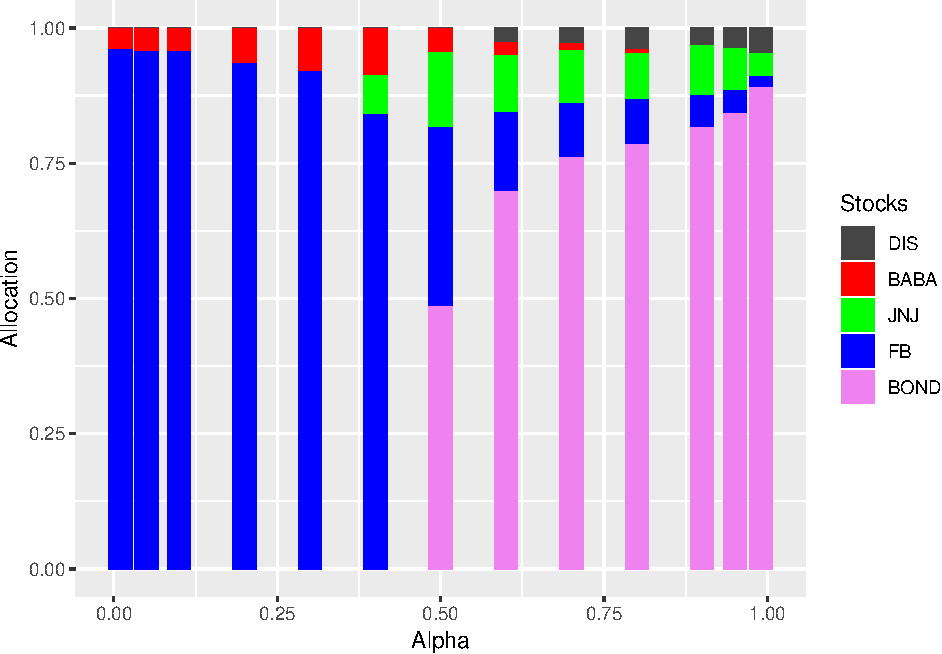
\includegraphics{Integrated_Management_Formulation_Model_files/figure-latex/unnamed-chunk-23-2.pdf}

\subsection{\texorpdfstring{Solving and asset allocation for
\(\gamma\)free =
0.3}{Solving and asset allocation for \textbackslash{}gammafree = 0.3}}\label{solving-and-asset-allocation-for-gammafree-0.3}

\begin{Shaded}
\begin{Highlighting}[]
\NormalTok{gammafree3 =}\StringTok{ }\FloatTok{0.3}
\NormalTok{dis_resultfree3 =}\StringTok{ }\KeywordTok{vector}\NormalTok{(}\DataTypeTok{mode =} \StringTok{"numeric"}\NormalTok{)}
\NormalTok{baba_resultfree3 =}\StringTok{ }\KeywordTok{vector}\NormalTok{(}\DataTypeTok{mode =} \StringTok{"numeric"}\NormalTok{)}
\NormalTok{jnj_resultfree3 =}\StringTok{ }\KeywordTok{vector}\NormalTok{(}\DataTypeTok{mode =} \StringTok{"numeric"}\NormalTok{)}
\NormalTok{fb_resultfree3 =}\StringTok{ }\KeywordTok{vector}\NormalTok{(}\DataTypeTok{mode =} \StringTok{"numeric"}\NormalTok{)}
\NormalTok{bond_resultfree3 =}\StringTok{ }\KeywordTok{vector}\NormalTok{(}\DataTypeTok{mode =} \StringTok{"numeric"}\NormalTok{)}
\ControlFlowTok{for}\NormalTok{ (alp }\ControlFlowTok{in}\NormalTok{ alpha)\{}
\NormalTok{  objvectfree3 <-}\StringTok{ }\KeywordTok{c}\NormalTok{((}\DecValTok{1}\OperatorTok{-}\NormalTok{gammafree3)}\OperatorTok{*}\KeywordTok{t}\NormalTok{(prob)}\OperatorTok\NormalTok{Portreturnsfree,(}\OperatorTok{-}\NormalTok{gammafree3}\OperatorTok{/}\NormalTok{(}\DecValTok{1}\OperatorTok{-}\NormalTok{alp))}\OperatorTok{*}\KeywordTok{t}\NormalTok{(prob),}\OperatorTok{-}\NormalTok{gammafree3)}
  \KeywordTok{names}\NormalTok{(objvectfree3)<-}\KeywordTok{c}\NormalTok{(}\StringTok{"dis"}\NormalTok{,}\StringTok{"baba"}\NormalTok{,}\StringTok{"jnj"}\NormalTok{,}\StringTok{"fb"}\NormalTok{,}\StringTok{"bond"}\NormalTok{,}\KeywordTok{rep}\NormalTok{(}\StringTok{"z"}\NormalTok{,}\DecValTok{826}\NormalTok{),}\StringTok{"q"}\NormalTok{) }
\NormalTok{  rhsconsfree3 <-}\StringTok{ }\KeywordTok{c}\NormalTok{(}\KeywordTok{rep}\NormalTok{(}\DecValTok{0}\NormalTok{,}\DecValTok{826}\NormalTok{ ),}\DecValTok{1}\NormalTok{,}\KeywordTok{rep}\NormalTok{(}\DecValTok{0}\NormalTok{,}\DecValTok{831}\NormalTok{))}
\CommentTok{#solution of the problem using linprog}
\NormalTok{  Solutionfree3 <-}\StringTok{ }\KeywordTok{solveLP}\NormalTok{(objvectfree3,rhsconsfree3,Amatfree,}\DataTypeTok{maximum =} \OtherTok{TRUE}\NormalTok{,}
          \DataTypeTok{const.dir =} \KeywordTok{c}\NormalTok{(}\KeywordTok{rep}\NormalTok{(}\StringTok{"<="}\NormalTok{,}\DecValTok{826}\NormalTok{),}\StringTok{"="}\NormalTok{,}\KeywordTok{rep}\NormalTok{(}\StringTok{"<="}\NormalTok{,}\DecValTok{831}\NormalTok{)),}\DataTypeTok{lpSolve =} \OtherTok{TRUE}\NormalTok{)}
\NormalTok{  dis_resultfree3<-}\KeywordTok{append}\NormalTok{(dis_resultfree3,Solutionfree3}\OperatorTok{$}\NormalTok{solution[}\DecValTok{1}\NormalTok{])}
\NormalTok{  baba_resultfree3<-}\StringTok{ }\KeywordTok{append}\NormalTok{(baba_resultfree3,Solutionfree3}\OperatorTok{$}\NormalTok{solution[}\DecValTok{2}\NormalTok{])}
\NormalTok{  jnj_resultfree3<-}\KeywordTok{append}\NormalTok{(jnj_resultfree3,Solutionfree3}\OperatorTok{$}\NormalTok{solution[}\DecValTok{3}\NormalTok{])}
\NormalTok{  fb_resultfree3<-}\KeywordTok{append}\NormalTok{(fb_resultfree3,Solutionfree3}\OperatorTok{$}\NormalTok{solution[}\DecValTok{4}\NormalTok{])}
\NormalTok{  bond_resultfree3<-}\KeywordTok{append}\NormalTok{(bond_resultfree3,Solutionfree3}\OperatorTok{$}\NormalTok{solution[}\DecValTok{5}\NormalTok{])}
\NormalTok{\}}
\NormalTok{  resultfree3 <-}\KeywordTok{data.frame}\NormalTok{(alpha,dis_resultfree3,baba_resultfree3,}
\NormalTok{                           jnj_resultfree3,fb_resultfree3,bond_resultfree3)}
  \KeywordTok{write.csv}\NormalTok{(resultfree3, }\DataTypeTok{file =} \StringTok{"Resultsfree3.csv"}\NormalTok{)}
  \KeywordTok{ggplot}\NormalTok{(resultfree3, }\KeywordTok{aes}\NormalTok{(}\DataTypeTok{x=}\NormalTok{resultfree3}\OperatorTok{$}\NormalTok{alpha)) }\OperatorTok{+}\StringTok{ }
\StringTok{    }\KeywordTok{geom_area}\NormalTok{(}\KeywordTok{aes}\NormalTok{(}\DataTypeTok{y=}\NormalTok{resultfree3}\OperatorTok{$}\NormalTok{dis_resultfree3}\OperatorTok{+}\NormalTok{resultfree3}\OperatorTok{$}\NormalTok{baba_resultfree3}\OperatorTok{+}
\StringTok{                    }\NormalTok{resultfree3}\OperatorTok{$}\NormalTok{jnj_resultfree3}\OperatorTok{+}\NormalTok{resultfree3}\OperatorTok{$}\NormalTok{fb_resultfree3}\OperatorTok{+}
\StringTok{                    }\NormalTok{resultfree3}\OperatorTok{$}\NormalTok{bond_resultfree3, }\DataTypeTok{fill=}\StringTok{"bond"}\NormalTok{))}\OperatorTok{+}
\StringTok{    }\KeywordTok{geom_area}\NormalTok{(}\KeywordTok{aes}\NormalTok{(}\DataTypeTok{y=}\NormalTok{resultfree3}\OperatorTok{$}\NormalTok{dis_resultfree3}\OperatorTok{+}\NormalTok{resultfree3}\OperatorTok{$}\NormalTok{baba_resultfree3}\OperatorTok{+}
\StringTok{                    }\NormalTok{resultfree3}\OperatorTok{$}\NormalTok{jnj_resultfree3}\OperatorTok{+}\NormalTok{resultfree3}\OperatorTok{$}\NormalTok{fb_resultfree3, }\DataTypeTok{fill=}\StringTok{"fb"}\NormalTok{)) }\OperatorTok{+}
\StringTok{    }\KeywordTok{geom_area}\NormalTok{(}\KeywordTok{aes}\NormalTok{(}\DataTypeTok{y=}\NormalTok{resultfree3}\OperatorTok{$}\NormalTok{dis_resultfree3}\OperatorTok{+}\NormalTok{resultfree3}\OperatorTok{$}\NormalTok{baba_resultfree3}\OperatorTok{+}
\StringTok{                    }\NormalTok{resultfree3}\OperatorTok{$}\NormalTok{jnj_resultfree3, }\DataTypeTok{fill=}\StringTok{"jnj"}\NormalTok{)) }\OperatorTok{+}
\StringTok{    }\KeywordTok{geom_area}\NormalTok{(}\KeywordTok{aes}\NormalTok{(}\DataTypeTok{y=}\NormalTok{resultfree3}\OperatorTok{$}\NormalTok{dis_resultfree3}\OperatorTok{+}\NormalTok{resultfree3}\OperatorTok{$}\NormalTok{baba_resultfree3,}\DataTypeTok{fill =} \StringTok{'baba'}\NormalTok{)) }\OperatorTok{+}
\StringTok{    }\KeywordTok{geom_area}\NormalTok{(}\KeywordTok{aes}\NormalTok{(}\DataTypeTok{y=}\NormalTok{resultfree3}\OperatorTok{$}\NormalTok{dis_resultfree3,}\DataTypeTok{fill =} \StringTok{"dis"}\NormalTok{))}\OperatorTok{+}
\StringTok{    }\KeywordTok{xlab}\NormalTok{(}\StringTok{"alpha levels"}\NormalTok{) }\OperatorTok{+}\StringTok{ }\KeywordTok{ylab}\NormalTok{(}\StringTok{"Weights on the stocks"}\NormalTok{) }\OperatorTok{+}
\StringTok{    }\KeywordTok{labs}\NormalTok{(}\DataTypeTok{title=}\StringTok{"Asset allocation for gamma = 0.3"}\NormalTok{) }\OperatorTok{+}\StringTok{  }\CommentTok{# title and caption}
\StringTok{    }\KeywordTok{scale_fill_manual}\NormalTok{(}\StringTok{"Stocks"}\NormalTok{,}
                      \DataTypeTok{values =}\KeywordTok{c}\NormalTok{(}\StringTok{"fb"}\NormalTok{=}\StringTok{"#0000FF"}\NormalTok{,}\StringTok{"jnj"}\NormalTok{=}\StringTok{"#00FF00"}\NormalTok{,}\StringTok{"baba"}\NormalTok{=}\StringTok{"#FF0000"}\NormalTok{,}\StringTok{"dis"}\NormalTok{=}\StringTok{"#454545"}\NormalTok{,}\StringTok{"bond"}\NormalTok{=}\StringTok{"violet"}\NormalTok{))}
\end{Highlighting}
\end{Shaded}

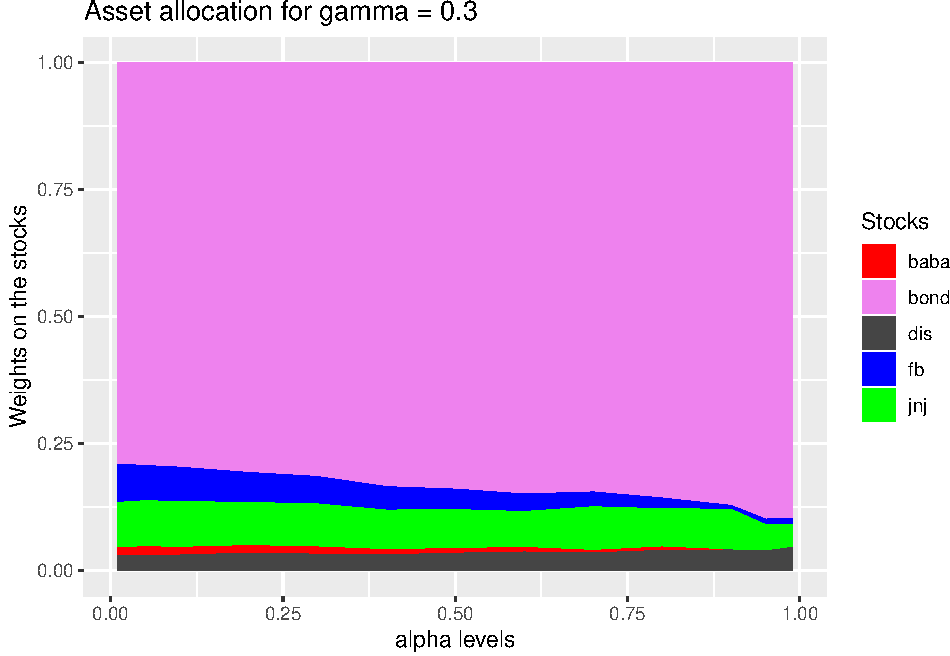
\includegraphics{Integrated_Management_Formulation_Model_files/figure-latex/unnamed-chunk-24-1.pdf}

\begin{Shaded}
\begin{Highlighting}[]
\CommentTok{# Using stacked barplots }
\KeywordTok{library}\NormalTok{(reshape2)}
\NormalTok{data3 <-}\StringTok{ }\NormalTok{resultfree3}
\KeywordTok{names}\NormalTok{(data3) <-}\StringTok{ }\KeywordTok{c}\NormalTok{(}\StringTok{"alpha"}\NormalTok{,}\StringTok{"DIS"}\NormalTok{,}\StringTok{"BABA"}\NormalTok{,}\StringTok{"JNJ"}\NormalTok{,}\StringTok{"FB"}\NormalTok{,}\StringTok{"BOND"}\NormalTok{)}
\NormalTok{mdata3 <-}\StringTok{ }\KeywordTok{melt}\NormalTok{(data3, }\DataTypeTok{id=}\KeywordTok{c}\NormalTok{(}\StringTok{"alpha"}\NormalTok{))}
\KeywordTok{names}\NormalTok{(mdata3) <-}\StringTok{ }\KeywordTok{c}\NormalTok{(}\StringTok{"Alpha"}\NormalTok{,}\StringTok{"Stocks"}\NormalTok{,}\StringTok{"Allocation"}\NormalTok{)}
\KeywordTok{ggplot}\NormalTok{() }\OperatorTok{+}\StringTok{ }\KeywordTok{geom_bar}\NormalTok{(}\KeywordTok{aes}\NormalTok{(}\DataTypeTok{y =}\NormalTok{ Allocation, }\DataTypeTok{x =}\NormalTok{ Alpha, }\DataTypeTok{fill =}\NormalTok{ Stocks), }\DataTypeTok{data =}\NormalTok{ mdata3, }\DataTypeTok{stat=}\StringTok{"identity"}\NormalTok{)}\OperatorTok{+}
\StringTok{  }\KeywordTok{scale_fill_manual}\NormalTok{(}\StringTok{"Stocks"}\NormalTok{,}\DataTypeTok{values =}
                      \KeywordTok{c}\NormalTok{(}\StringTok{"FB"}\NormalTok{=}\StringTok{"#0000FF"}\NormalTok{,}\StringTok{"JNJ"}\NormalTok{=}\StringTok{"#00FF00"}\NormalTok{,}\StringTok{"BABA"}\NormalTok{=}\StringTok{"#FF0000"}\NormalTok{,}\StringTok{"DIS"}\NormalTok{=}\StringTok{"#454545"}\NormalTok{,}\StringTok{"BOND"}\NormalTok{ =}\StringTok{ "violet"}\NormalTok{))}
\end{Highlighting}
\end{Shaded}

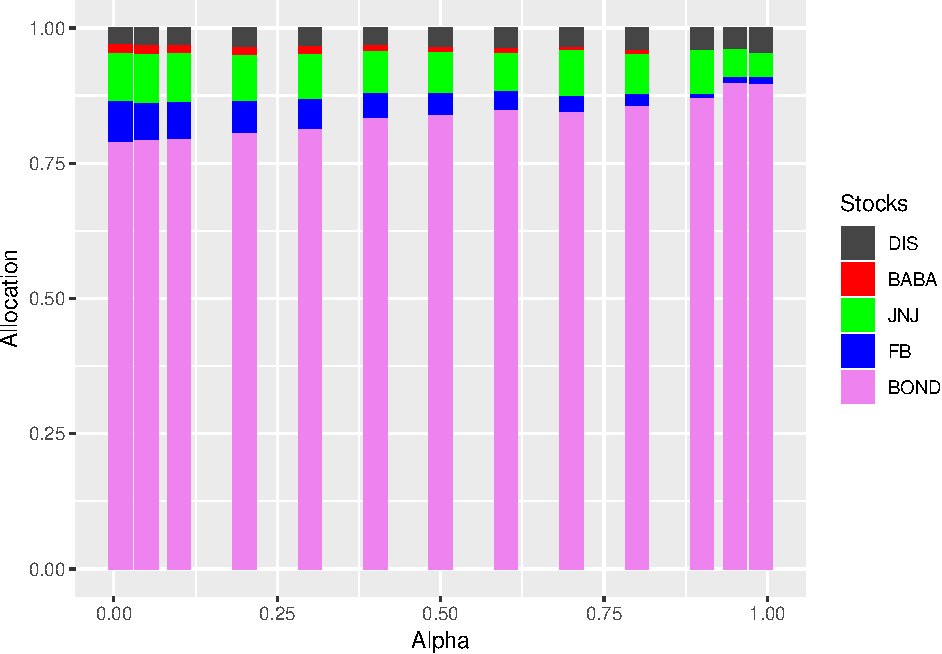
\includegraphics{Integrated_Management_Formulation_Model_files/figure-latex/unnamed-chunk-24-2.pdf}

\subsection{\texorpdfstring{Solving and asset allocation for
\(\gamma\)free =
0.5}{Solving and asset allocation for \textbackslash{}gammafree = 0.5}}\label{solving-and-asset-allocation-for-gammafree-0.5}

\begin{Shaded}
\begin{Highlighting}[]
\NormalTok{gammafree5 =}\StringTok{ }\FloatTok{0.5}
\NormalTok{dis_resultfree5 <-}\StringTok{ }\KeywordTok{vector}\NormalTok{(}\DataTypeTok{mode =} \StringTok{"numeric"}\NormalTok{)}
\NormalTok{baba_resultfree5 <-}\StringTok{ }\KeywordTok{vector}\NormalTok{(}\DataTypeTok{mode =} \StringTok{"numeric"}\NormalTok{)}
\NormalTok{jnj_resultfree5 <-}\StringTok{ }\KeywordTok{vector}\NormalTok{(}\DataTypeTok{mode =} \StringTok{"numeric"}\NormalTok{)}
\NormalTok{fb_resultfree5 <-}\StringTok{ }\KeywordTok{vector}\NormalTok{(}\DataTypeTok{mode =} \StringTok{"numeric"}\NormalTok{)}
\NormalTok{bond_resultfree5 <-}\StringTok{ }\KeywordTok{vector}\NormalTok{(}\DataTypeTok{mode =} \StringTok{"numeric"}\NormalTok{)}
\ControlFlowTok{for}\NormalTok{ (alp }\ControlFlowTok{in}\NormalTok{ alpha)\{}
\NormalTok{  objvectfree5 <-}\StringTok{ }\KeywordTok{c}\NormalTok{((}\DecValTok{1}\OperatorTok{-}\NormalTok{gammafree5)}\OperatorTok{*}\KeywordTok{t}\NormalTok{(prob)}\OperatorTok\NormalTok{Portreturnsfree,(}\OperatorTok{-}\NormalTok{gammafree5}\OperatorTok{/}\NormalTok{(}\DecValTok{1}\OperatorTok{-}\NormalTok{alp))}\OperatorTok{*}\KeywordTok{t}\NormalTok{(prob),}\OperatorTok{-}\NormalTok{gammafree5)}
  \KeywordTok{names}\NormalTok{(objvectfree5)<-}\KeywordTok{c}\NormalTok{(}\StringTok{"dis"}\NormalTok{,}\StringTok{"baba"}\NormalTok{,}\StringTok{"jnj"}\NormalTok{,}\StringTok{"fb"}\NormalTok{,}\StringTok{"bond"}\NormalTok{,}\KeywordTok{rep}\NormalTok{(}\StringTok{"z"}\NormalTok{,}\DecValTok{826}\NormalTok{),}\StringTok{"q"}\NormalTok{) }
\NormalTok{  rhsconsfree5 <-}\StringTok{ }\KeywordTok{c}\NormalTok{(}\KeywordTok{rep}\NormalTok{(}\DecValTok{0}\NormalTok{,}\DecValTok{826}\NormalTok{ ),}\DecValTok{1}\NormalTok{,}\KeywordTok{rep}\NormalTok{(}\DecValTok{0}\NormalTok{,}\DecValTok{831}\NormalTok{))}
\NormalTok{  Solutionfree5 <-}\StringTok{ }\KeywordTok{solveLP}\NormalTok{(objvectfree5,rhsconsfree5,Amatfree,}\DataTypeTok{maximum =} \OtherTok{TRUE}\NormalTok{,}
          \DataTypeTok{const.dir =} \KeywordTok{c}\NormalTok{(}\KeywordTok{rep}\NormalTok{(}\StringTok{"<="}\NormalTok{,}\DecValTok{826}\NormalTok{),}\StringTok{"="}\NormalTok{,}\KeywordTok{rep}\NormalTok{(}\StringTok{"<="}\NormalTok{,}\DecValTok{831}\NormalTok{)),}\DataTypeTok{lpSolve =} \OtherTok{TRUE}\NormalTok{)}
\NormalTok{  dis_resultfree5<-}\KeywordTok{append}\NormalTok{(dis_resultfree5,Solutionfree5}\OperatorTok{$}\NormalTok{solution[}\DecValTok{1}\NormalTok{])}
\NormalTok{  baba_resultfree5<-}\StringTok{ }\KeywordTok{append}\NormalTok{(baba_resultfree5,Solutionfree5}\OperatorTok{$}\NormalTok{solution[}\DecValTok{2}\NormalTok{])}
\NormalTok{  jnj_resultfree5<-}\KeywordTok{append}\NormalTok{(jnj_resultfree5,Solutionfree5}\OperatorTok{$}\NormalTok{solution[}\DecValTok{3}\NormalTok{])}
\NormalTok{  fb_resultfree5<-}\KeywordTok{append}\NormalTok{(fb_resultfree5,Solutionfree5}\OperatorTok{$}\NormalTok{solution[}\DecValTok{4}\NormalTok{])}
\NormalTok{  bond_resultfree5<-}\KeywordTok{append}\NormalTok{(bond_resultfree5,Solutionfree5}\OperatorTok{$}\NormalTok{solution[}\DecValTok{5}\NormalTok{])}
\NormalTok{\}}
\NormalTok{  resultfree5 <-}\KeywordTok{data.frame}\NormalTok{(alpha,dis_resultfree5,baba_resultfree5,}
\NormalTok{                           jnj_resultfree5,fb_resultfree5,bond_resultfree5)}
  \KeywordTok{write.csv}\NormalTok{(resultfree5, }\DataTypeTok{file =} \StringTok{"Resultsfree5.csv"}\NormalTok{)}
  \KeywordTok{ggplot}\NormalTok{(resultfree5, }\KeywordTok{aes}\NormalTok{(}\DataTypeTok{x=}\NormalTok{resultfree5}\OperatorTok{$}\NormalTok{alpha)) }\OperatorTok{+}\StringTok{ }
\StringTok{    }\KeywordTok{geom_area}\NormalTok{(}\KeywordTok{aes}\NormalTok{(}\DataTypeTok{y=}\NormalTok{resultfree5}\OperatorTok{$}\NormalTok{dis_resultfree5}\OperatorTok{+}\NormalTok{resultfree5}\OperatorTok{$}\NormalTok{baba_resultfree5}\OperatorTok{+}
\StringTok{                    }\NormalTok{resultfree5}\OperatorTok{$}\NormalTok{jnj_resultfree5}\OperatorTok{+}\NormalTok{resultfree5}\OperatorTok{$}\NormalTok{fb_resultfree5}\OperatorTok{+}
\StringTok{                    }\NormalTok{resultfree5}\OperatorTok{$}\NormalTok{bond_resultfree5, }\DataTypeTok{fill=}\StringTok{"bond"}\NormalTok{))}\OperatorTok{+}
\StringTok{    }\KeywordTok{geom_area}\NormalTok{(}\KeywordTok{aes}\NormalTok{(}\DataTypeTok{y=}\NormalTok{resultfree5}\OperatorTok{$}\NormalTok{dis_resultfree5}\OperatorTok{+}\NormalTok{resultfree5}\OperatorTok{$}\NormalTok{baba_resultfree5}\OperatorTok{+}
\StringTok{                    }\NormalTok{resultfree5}\OperatorTok{$}\NormalTok{jnj_resultfree5}\OperatorTok{+}\NormalTok{resultfree5}\OperatorTok{$}\NormalTok{fb_resultfree5, }\DataTypeTok{fill=}\StringTok{"fb"}\NormalTok{)) }\OperatorTok{+}
\StringTok{    }\KeywordTok{geom_area}\NormalTok{(}\KeywordTok{aes}\NormalTok{(}\DataTypeTok{y=}\NormalTok{resultfree5}\OperatorTok{$}\NormalTok{dis_resultfree5}\OperatorTok{+}\NormalTok{resultfree5}\OperatorTok{$}\NormalTok{baba_resultfree5}\OperatorTok{+}
\StringTok{                    }\NormalTok{resultfree5}\OperatorTok{$}\NormalTok{jnj_resultfree5, }\DataTypeTok{fill=}\StringTok{"jnj"}\NormalTok{)) }\OperatorTok{+}
\StringTok{    }\KeywordTok{geom_area}\NormalTok{(}\KeywordTok{aes}\NormalTok{(}\DataTypeTok{y=}\NormalTok{resultfree5}\OperatorTok{$}\NormalTok{dis_resultfree5}\OperatorTok{+}\NormalTok{resultfree5}\OperatorTok{$}\NormalTok{baba_resultfree5,}\DataTypeTok{fill =} \StringTok{'baba'}\NormalTok{)) }\OperatorTok{+}
\StringTok{    }\KeywordTok{geom_area}\NormalTok{(}\KeywordTok{aes}\NormalTok{(}\DataTypeTok{y=}\NormalTok{resultfree5}\OperatorTok{$}\NormalTok{dis_resultfree5,}\DataTypeTok{fill =} \StringTok{"dis"}\NormalTok{))}\OperatorTok{+}
\StringTok{    }\KeywordTok{xlab}\NormalTok{(}\StringTok{"alpha levels"}\NormalTok{) }\OperatorTok{+}\StringTok{ }\KeywordTok{ylab}\NormalTok{(}\StringTok{"Weights on the stocks"}\NormalTok{) }\OperatorTok{+}
\StringTok{    }\KeywordTok{labs}\NormalTok{(}\DataTypeTok{title=}\StringTok{"Asset allocation for gamma = 0.5"}\NormalTok{) }\OperatorTok{+}\StringTok{  }\CommentTok{# title and caption}
\StringTok{    }\KeywordTok{scale_fill_manual}\NormalTok{(}\StringTok{"Stocks"}\NormalTok{,}
                      \DataTypeTok{values =}\KeywordTok{c}\NormalTok{(}\StringTok{"fb"}\NormalTok{=}\StringTok{"#0000FF"}\NormalTok{,}\StringTok{"jnj"}\NormalTok{=}\StringTok{"#00FF00"}\NormalTok{,}\StringTok{"baba"}\NormalTok{=}\StringTok{"#FF0000"}\NormalTok{,}\StringTok{"dis"}\NormalTok{=}\StringTok{"#454545"}\NormalTok{,}\StringTok{"bond"}\NormalTok{=}\StringTok{"violet"}\NormalTok{))}
\end{Highlighting}
\end{Shaded}

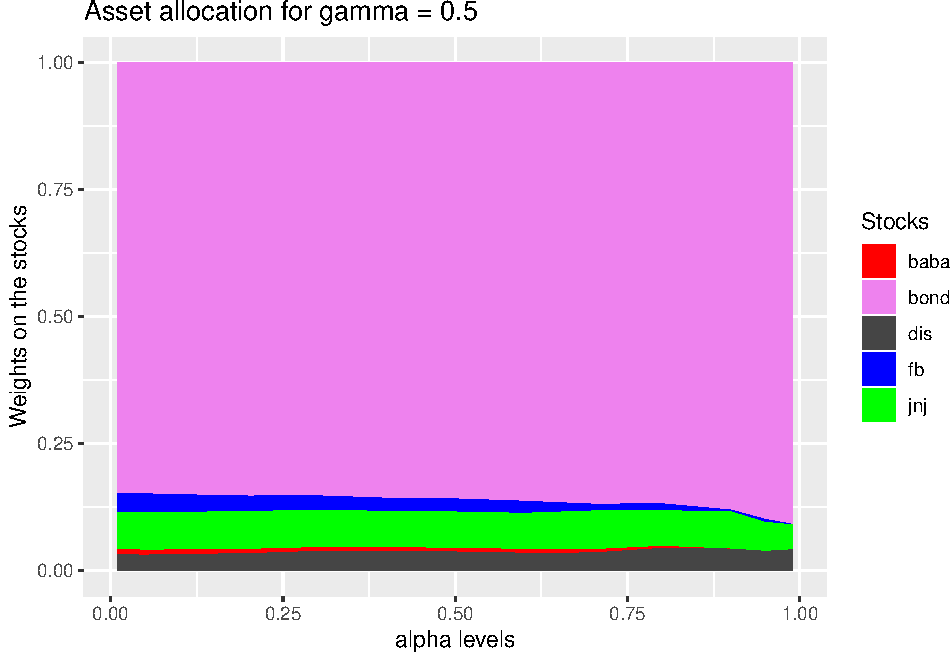
\includegraphics{Integrated_Management_Formulation_Model_files/figure-latex/unnamed-chunk-25-1.pdf}

\begin{Shaded}
\begin{Highlighting}[]
\CommentTok{# Using stacked barplots }
\KeywordTok{library}\NormalTok{(reshape2)}
\NormalTok{data5 <-}\StringTok{ }\NormalTok{resultfree5}
\KeywordTok{names}\NormalTok{(data5) <-}\StringTok{ }\KeywordTok{c}\NormalTok{(}\StringTok{"alpha"}\NormalTok{,}\StringTok{"DIS"}\NormalTok{,}\StringTok{"BABA"}\NormalTok{,}\StringTok{"JNJ"}\NormalTok{,}\StringTok{"FB"}\NormalTok{,}\StringTok{"BOND"}\NormalTok{)}
\NormalTok{mdata5 <-}\StringTok{ }\KeywordTok{melt}\NormalTok{(data5, }\DataTypeTok{id=}\KeywordTok{c}\NormalTok{(}\StringTok{"alpha"}\NormalTok{))}
\KeywordTok{names}\NormalTok{(mdata5) <-}\StringTok{ }\KeywordTok{c}\NormalTok{(}\StringTok{"Alpha"}\NormalTok{,}\StringTok{"Stocks"}\NormalTok{,}\StringTok{"Allocation"}\NormalTok{)}
\KeywordTok{ggplot}\NormalTok{() }\OperatorTok{+}\StringTok{ }\KeywordTok{geom_bar}\NormalTok{(}\KeywordTok{aes}\NormalTok{(}\DataTypeTok{y =}\NormalTok{ Allocation, }\DataTypeTok{x =}\NormalTok{ Alpha, }\DataTypeTok{fill =}\NormalTok{ Stocks), }\DataTypeTok{data =}\NormalTok{ mdata5, }\DataTypeTok{stat=}\StringTok{"identity"}\NormalTok{)}\OperatorTok{+}
\StringTok{  }\KeywordTok{scale_fill_manual}\NormalTok{(}\StringTok{"Stocks"}\NormalTok{,}\DataTypeTok{values =}
                      \KeywordTok{c}\NormalTok{(}\StringTok{"FB"}\NormalTok{=}\StringTok{"#0000FF"}\NormalTok{,}\StringTok{"JNJ"}\NormalTok{=}\StringTok{"#00FF00"}\NormalTok{,}\StringTok{"BABA"}\NormalTok{=}\StringTok{"#FF0000"}\NormalTok{,}\StringTok{"DIS"}\NormalTok{=}\StringTok{"#454545"}\NormalTok{,}\StringTok{"BOND"}\NormalTok{ =}\StringTok{ "violet"}\NormalTok{))}
\end{Highlighting}
\end{Shaded}

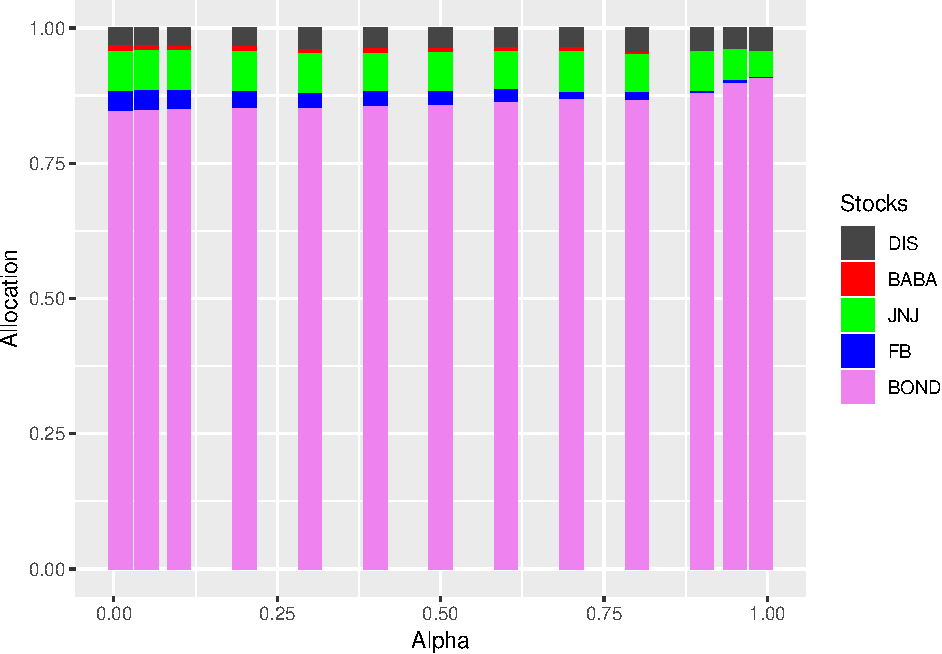
\includegraphics{Integrated_Management_Formulation_Model_files/figure-latex/unnamed-chunk-25-2.pdf}

\subsection{\texorpdfstring{Solving and asset allocation for
\(\gamma\)free =
0.7}{Solving and asset allocation for \textbackslash{}gammafree = 0.7}}\label{solving-and-asset-allocation-for-gammafree-0.7}

\begin{Shaded}
\begin{Highlighting}[]
\NormalTok{gammafree7 =}\StringTok{ }\FloatTok{0.7}
\NormalTok{dis_resultfree7 =}\StringTok{ }\KeywordTok{vector}\NormalTok{(}\DataTypeTok{mode =} \StringTok{"numeric"}\NormalTok{)}
\NormalTok{baba_resultfree7 =}\StringTok{ }\KeywordTok{vector}\NormalTok{(}\DataTypeTok{mode =} \StringTok{"numeric"}\NormalTok{)}
\NormalTok{jnj_resultfree7 =}\StringTok{ }\KeywordTok{vector}\NormalTok{(}\DataTypeTok{mode =} \StringTok{"numeric"}\NormalTok{)}
\NormalTok{fb_resultfree7 =}\StringTok{ }\KeywordTok{vector}\NormalTok{(}\DataTypeTok{mode =} \StringTok{"numeric"}\NormalTok{)}
\NormalTok{bond_resultfree7 =}\StringTok{ }\KeywordTok{vector}\NormalTok{(}\DataTypeTok{mode =} \StringTok{"numeric"}\NormalTok{)}
\ControlFlowTok{for}\NormalTok{ (alp }\ControlFlowTok{in}\NormalTok{ alpha)\{}
\NormalTok{  objvectfree7 <-}\StringTok{ }\KeywordTok{c}\NormalTok{((}\DecValTok{1}\OperatorTok{-}\NormalTok{gammafree7)}\OperatorTok{*}\KeywordTok{t}\NormalTok{(prob)}\OperatorTok\NormalTok{Portreturnsfree,(}\OperatorTok{-}\NormalTok{gammafree7}\OperatorTok{/}\NormalTok{(}\DecValTok{1}\OperatorTok{-}\NormalTok{alp))}\OperatorTok{*}\KeywordTok{t}\NormalTok{(prob),}\OperatorTok{-}\NormalTok{gammafree7)}
  \KeywordTok{names}\NormalTok{(objvectfree7)<-}\KeywordTok{c}\NormalTok{(}\StringTok{"dis"}\NormalTok{,}\StringTok{"baba"}\NormalTok{,}\StringTok{"jnj"}\NormalTok{,}\StringTok{"fb"}\NormalTok{,}\StringTok{"bond"}\NormalTok{,}\KeywordTok{rep}\NormalTok{(}\StringTok{"z"}\NormalTok{,}\DecValTok{826}\NormalTok{),}\StringTok{"q"}\NormalTok{) }
\NormalTok{  rhsconsfree7 <-}\StringTok{ }\KeywordTok{c}\NormalTok{(}\KeywordTok{rep}\NormalTok{(}\DecValTok{0}\NormalTok{,}\DecValTok{826}\NormalTok{ ),}\DecValTok{1}\NormalTok{,}\KeywordTok{rep}\NormalTok{(}\DecValTok{0}\NormalTok{,}\DecValTok{831}\NormalTok{))}
\NormalTok{  Solutionfree7 <-}\StringTok{ }\KeywordTok{solveLP}\NormalTok{(objvectfree7,rhsconsfree7,Amatfree,}\DataTypeTok{maximum =} \OtherTok{TRUE}\NormalTok{,}
          \DataTypeTok{const.dir =} \KeywordTok{c}\NormalTok{(}\KeywordTok{rep}\NormalTok{(}\StringTok{"<="}\NormalTok{,}\DecValTok{826}\NormalTok{),}\StringTok{"="}\NormalTok{,}\KeywordTok{rep}\NormalTok{(}\StringTok{"<="}\NormalTok{,}\DecValTok{831}\NormalTok{)),}\DataTypeTok{lpSolve =} \OtherTok{TRUE}\NormalTok{)}
\NormalTok{  dis_resultfree7<-}\KeywordTok{append}\NormalTok{(dis_resultfree7,Solutionfree7}\OperatorTok{$}\NormalTok{solution[}\DecValTok{1}\NormalTok{])}
\NormalTok{  baba_resultfree7<-}\StringTok{ }\KeywordTok{append}\NormalTok{(baba_resultfree7,Solutionfree7}\OperatorTok{$}\NormalTok{solution[}\DecValTok{2}\NormalTok{])}
\NormalTok{  jnj_resultfree7<-}\KeywordTok{append}\NormalTok{(jnj_resultfree7,Solutionfree7}\OperatorTok{$}\NormalTok{solution[}\DecValTok{3}\NormalTok{])}
\NormalTok{  fb_resultfree7<-}\KeywordTok{append}\NormalTok{(fb_resultfree7,Solutionfree7}\OperatorTok{$}\NormalTok{solution[}\DecValTok{4}\NormalTok{])}
\NormalTok{  bond_resultfree7<-}\KeywordTok{append}\NormalTok{(bond_resultfree7,Solutionfree7}\OperatorTok{$}\NormalTok{solution[}\DecValTok{5}\NormalTok{])}
\NormalTok{\}}
\NormalTok{  resultfree7 <-}\KeywordTok{data.frame}\NormalTok{(alpha,dis_resultfree7,baba_resultfree7,}
\NormalTok{                           jnj_resultfree7,fb_resultfree7,bond_resultfree7)}
  \KeywordTok{write.csv}\NormalTok{(resultfree7, }\DataTypeTok{file =} \StringTok{"Resultsfree7.csv"}\NormalTok{)}
  \KeywordTok{ggplot}\NormalTok{(resultfree7, }\KeywordTok{aes}\NormalTok{(}\DataTypeTok{x=}\NormalTok{resultfree7}\OperatorTok{$}\NormalTok{alpha)) }\OperatorTok{+}\StringTok{ }
\StringTok{    }\KeywordTok{geom_area}\NormalTok{(}\KeywordTok{aes}\NormalTok{(}\DataTypeTok{y=}\NormalTok{resultfree7}\OperatorTok{$}\NormalTok{dis_resultfree7}\OperatorTok{+}\NormalTok{resultfree7}\OperatorTok{$}\NormalTok{baba_resultfree7}\OperatorTok{+}
\StringTok{                    }\NormalTok{resultfree7}\OperatorTok{$}\NormalTok{jnj_resultfree7}\OperatorTok{+}\NormalTok{resultfree7}\OperatorTok{$}\NormalTok{fb_resultfree7}\OperatorTok{+}
\StringTok{                    }\NormalTok{resultfree7}\OperatorTok{$}\NormalTok{bond_resultfree7, }\DataTypeTok{fill=}\StringTok{"bond"}\NormalTok{))}\OperatorTok{+}
\StringTok{    }\KeywordTok{geom_area}\NormalTok{(}\KeywordTok{aes}\NormalTok{(}\DataTypeTok{y=}\NormalTok{resultfree7}\OperatorTok{$}\NormalTok{dis_resultfree7}\OperatorTok{+}\NormalTok{resultfree7}\OperatorTok{$}\NormalTok{baba_resultfree7}\OperatorTok{+}
\StringTok{                    }\NormalTok{resultfree7}\OperatorTok{$}\NormalTok{jnj_resultfree7}\OperatorTok{+}\NormalTok{resultfree7}\OperatorTok{$}\NormalTok{fb_resultfree7, }\DataTypeTok{fill=}\StringTok{"fb"}\NormalTok{)) }\OperatorTok{+}
\StringTok{    }\KeywordTok{geom_area}\NormalTok{(}\KeywordTok{aes}\NormalTok{(}\DataTypeTok{y=}\NormalTok{resultfree7}\OperatorTok{$}\NormalTok{dis_resultfree7}\OperatorTok{+}\NormalTok{resultfree7}\OperatorTok{$}\NormalTok{baba_resultfree7}\OperatorTok{+}
\StringTok{                    }\NormalTok{resultfree7}\OperatorTok{$}\NormalTok{jnj_resultfree7, }\DataTypeTok{fill=}\StringTok{"jnj"}\NormalTok{)) }\OperatorTok{+}
\StringTok{    }\KeywordTok{geom_area}\NormalTok{(}\KeywordTok{aes}\NormalTok{(}\DataTypeTok{y=}\NormalTok{resultfree7}\OperatorTok{$}\NormalTok{dis_resultfree7}\OperatorTok{+}\NormalTok{resultfree7}\OperatorTok{$}\NormalTok{baba_resultfree7,}\DataTypeTok{fill =} \StringTok{'baba'}\NormalTok{)) }\OperatorTok{+}
\StringTok{    }\KeywordTok{geom_area}\NormalTok{(}\KeywordTok{aes}\NormalTok{(}\DataTypeTok{y=}\NormalTok{resultfree7}\OperatorTok{$}\NormalTok{dis_resultfree7,}\DataTypeTok{fill =} \StringTok{"dis"}\NormalTok{))}\OperatorTok{+}
\StringTok{    }\KeywordTok{xlab}\NormalTok{(}\StringTok{"alpha levels"}\NormalTok{) }\OperatorTok{+}\StringTok{ }\KeywordTok{ylab}\NormalTok{(}\StringTok{"Weights on the stocks"}\NormalTok{) }\OperatorTok{+}
\StringTok{    }\KeywordTok{labs}\NormalTok{(}\DataTypeTok{title=}\StringTok{"Asset allocation for gamma = 0.7"}\NormalTok{) }\OperatorTok{+}\StringTok{  }\CommentTok{# title and caption}
\StringTok{    }\KeywordTok{scale_fill_manual}\NormalTok{(}\StringTok{"Stocks"}\NormalTok{,}
                      \DataTypeTok{values =}\KeywordTok{c}\NormalTok{(}\StringTok{"fb"}\NormalTok{=}\StringTok{"#0000FF"}\NormalTok{,}\StringTok{"jnj"}\NormalTok{=}\StringTok{"#00FF00"}\NormalTok{,}\StringTok{"baba"}\NormalTok{=}\StringTok{"#FF0000"}\NormalTok{,}\StringTok{"dis"}\NormalTok{=}\StringTok{"#454545"}\NormalTok{,}\StringTok{"bond"}\NormalTok{=}\StringTok{"violet"}\NormalTok{))}
\end{Highlighting}
\end{Shaded}

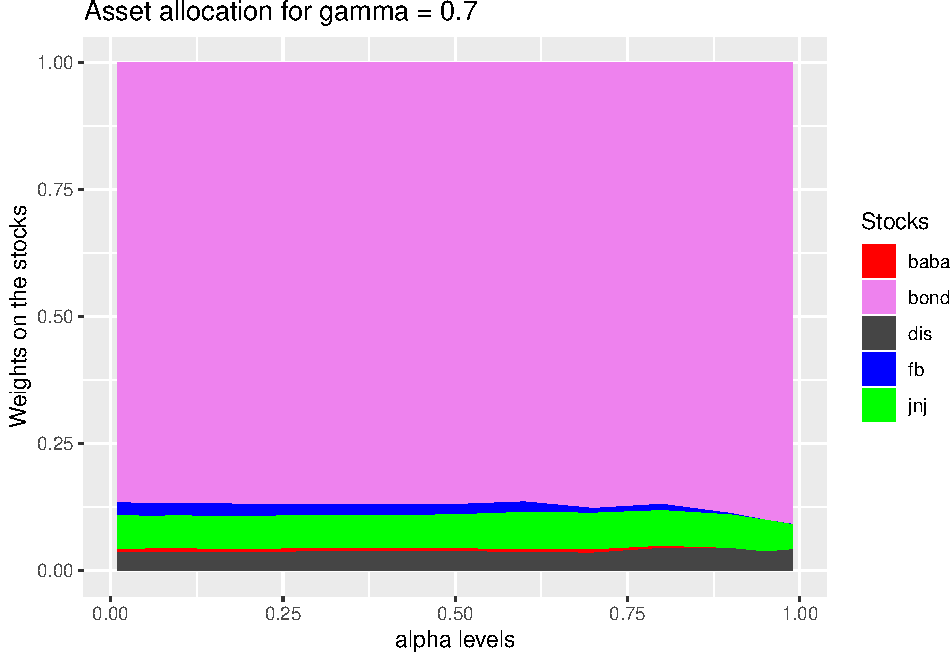
\includegraphics{Integrated_Management_Formulation_Model_files/figure-latex/unnamed-chunk-26-1.pdf}

\begin{Shaded}
\begin{Highlighting}[]
\CommentTok{# Using stacked barplots }
\KeywordTok{library}\NormalTok{(reshape2)}
\NormalTok{data7 <-}\StringTok{ }\NormalTok{resultfree7}
\KeywordTok{names}\NormalTok{(data7) <-}\StringTok{ }\KeywordTok{c}\NormalTok{(}\StringTok{"alpha"}\NormalTok{,}\StringTok{"DIS"}\NormalTok{,}\StringTok{"BABA"}\NormalTok{,}\StringTok{"JNJ"}\NormalTok{,}\StringTok{"FB"}\NormalTok{,}\StringTok{"BOND"}\NormalTok{)}
\NormalTok{mdata7 <-}\StringTok{ }\KeywordTok{melt}\NormalTok{(data7, }\DataTypeTok{id=}\KeywordTok{c}\NormalTok{(}\StringTok{"alpha"}\NormalTok{))}
\KeywordTok{names}\NormalTok{(mdata7) <-}\StringTok{ }\KeywordTok{c}\NormalTok{(}\StringTok{"Alpha"}\NormalTok{,}\StringTok{"Stocks"}\NormalTok{,}\StringTok{"Allocation"}\NormalTok{)}
\KeywordTok{ggplot}\NormalTok{() }\OperatorTok{+}\StringTok{ }\KeywordTok{geom_bar}\NormalTok{(}\KeywordTok{aes}\NormalTok{(}\DataTypeTok{y =}\NormalTok{ Allocation, }\DataTypeTok{x =}\NormalTok{ Alpha, }\DataTypeTok{fill =}\NormalTok{ Stocks), }\DataTypeTok{data =}\NormalTok{ mdata7, }\DataTypeTok{stat=}\StringTok{"identity"}\NormalTok{)}\OperatorTok{+}
\StringTok{  }\KeywordTok{scale_fill_manual}\NormalTok{(}\StringTok{"Stocks"}\NormalTok{,}\DataTypeTok{values =}
                      \KeywordTok{c}\NormalTok{(}\StringTok{"FB"}\NormalTok{=}\StringTok{"#0000FF"}\NormalTok{,}\StringTok{"JNJ"}\NormalTok{=}\StringTok{"#00FF00"}\NormalTok{,}\StringTok{"BABA"}\NormalTok{=}\StringTok{"#FF0000"}\NormalTok{,}\StringTok{"DIS"}\NormalTok{=}\StringTok{"#454545"}\NormalTok{,}\StringTok{"BOND"}\NormalTok{ =}\StringTok{ "violet"}\NormalTok{))}
\end{Highlighting}
\end{Shaded}

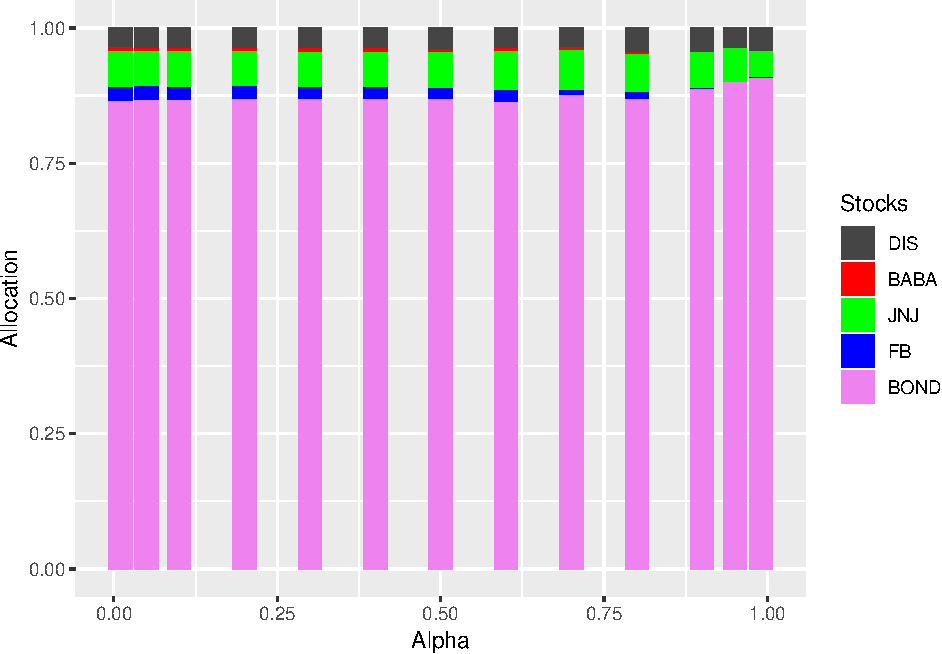
\includegraphics{Integrated_Management_Formulation_Model_files/figure-latex/unnamed-chunk-26-2.pdf}

\subsection{\texorpdfstring{Solving and asset allocation for
\(\gamma\)free =
0.9}{Solving and asset allocation for \textbackslash{}gammafree = 0.9}}\label{solving-and-asset-allocation-for-gammafree-0.9}

\begin{Shaded}
\begin{Highlighting}[]
\NormalTok{gammafree9 =}\StringTok{ }\FloatTok{0.9}
\NormalTok{dis_resultfree9 =}\StringTok{ }\KeywordTok{vector}\NormalTok{(}\DataTypeTok{mode =} \StringTok{"numeric"}\NormalTok{)}
\NormalTok{baba_resultfree9 =}\StringTok{ }\KeywordTok{vector}\NormalTok{(}\DataTypeTok{mode =} \StringTok{"numeric"}\NormalTok{)}
\NormalTok{jnj_resultfree9 =}\StringTok{ }\KeywordTok{vector}\NormalTok{(}\DataTypeTok{mode =} \StringTok{"numeric"}\NormalTok{)}
\NormalTok{fb_resultfree9 =}\StringTok{ }\KeywordTok{vector}\NormalTok{(}\DataTypeTok{mode =} \StringTok{"numeric"}\NormalTok{)}
\NormalTok{bond_resultfree9 =}\StringTok{ }\KeywordTok{vector}\NormalTok{(}\DataTypeTok{mode =} \StringTok{"numeric"}\NormalTok{)}
\ControlFlowTok{for}\NormalTok{ (alp }\ControlFlowTok{in}\NormalTok{ alpha)\{}
\NormalTok{  objvectfree9 <-}\StringTok{ }\KeywordTok{c}\NormalTok{((}\DecValTok{1}\OperatorTok{-}\NormalTok{gammafree9)}\OperatorTok{*}\KeywordTok{t}\NormalTok{(prob)}\OperatorTok\NormalTok{Portreturnsfree,(}\OperatorTok{-}\NormalTok{gammafree9}\OperatorTok{/}\NormalTok{(}\DecValTok{1}\OperatorTok{-}\NormalTok{alp))}\OperatorTok{*}\KeywordTok{t}\NormalTok{(prob),}\OperatorTok{-}\NormalTok{gammafree9)}
  \KeywordTok{names}\NormalTok{(objvectfree9)<-}\KeywordTok{c}\NormalTok{(}\StringTok{"dis"}\NormalTok{,}\StringTok{"baba"}\NormalTok{,}\StringTok{"jnj"}\NormalTok{,}\StringTok{"fb"}\NormalTok{,}\StringTok{"bond"}\NormalTok{,}\KeywordTok{rep}\NormalTok{(}\StringTok{"z"}\NormalTok{,}\DecValTok{826}\NormalTok{),}\StringTok{"q"}\NormalTok{) }
\NormalTok{  rhsconsfree9 <-}\StringTok{ }\KeywordTok{c}\NormalTok{(}\KeywordTok{rep}\NormalTok{(}\DecValTok{0}\NormalTok{,}\DecValTok{826}\NormalTok{ ),}\DecValTok{1}\NormalTok{,}\KeywordTok{rep}\NormalTok{(}\DecValTok{0}\NormalTok{,}\DecValTok{831}\NormalTok{))}
\NormalTok{  Solutionfree9 <-}\StringTok{ }\KeywordTok{solveLP}\NormalTok{(objvectfree9,rhsconsfree9,Amatfree,}\DataTypeTok{maximum =} \OtherTok{TRUE}\NormalTok{,}
          \DataTypeTok{const.dir =} \KeywordTok{c}\NormalTok{(}\KeywordTok{rep}\NormalTok{(}\StringTok{"<="}\NormalTok{,}\DecValTok{826}\NormalTok{),}\StringTok{"="}\NormalTok{,}\KeywordTok{rep}\NormalTok{(}\StringTok{"<="}\NormalTok{,}\DecValTok{831}\NormalTok{)),}\DataTypeTok{lpSolve =} \OtherTok{TRUE}\NormalTok{)}
\NormalTok{  dis_resultfree9<-}\KeywordTok{append}\NormalTok{(dis_resultfree9,Solutionfree9}\OperatorTok{$}\NormalTok{solution[}\DecValTok{1}\NormalTok{])}
\NormalTok{  baba_resultfree9<-}\StringTok{ }\KeywordTok{append}\NormalTok{(baba_resultfree9,Solutionfree9}\OperatorTok{$}\NormalTok{solution[}\DecValTok{2}\NormalTok{])}
\NormalTok{  jnj_resultfree9<-}\KeywordTok{append}\NormalTok{(jnj_resultfree9,Solutionfree9}\OperatorTok{$}\NormalTok{solution[}\DecValTok{3}\NormalTok{])}
\NormalTok{  fb_resultfree9<-}\KeywordTok{append}\NormalTok{(fb_resultfree9,Solutionfree9}\OperatorTok{$}\NormalTok{solution[}\DecValTok{4}\NormalTok{])}
\NormalTok{  bond_resultfree9<-}\KeywordTok{append}\NormalTok{(bond_resultfree9,Solutionfree9}\OperatorTok{$}\NormalTok{solution[}\DecValTok{5}\NormalTok{])}
\NormalTok{\}}
\NormalTok{  resultfree9 <-}\KeywordTok{data.frame}\NormalTok{(alpha,dis_resultfree9,baba_resultfree9,}
\NormalTok{                           jnj_resultfree9,fb_resultfree9,bond_resultfree9)}
  \KeywordTok{write.csv}\NormalTok{(resultfree9, }\DataTypeTok{file =} \StringTok{"Resultsfree9.csv"}\NormalTok{)}
  \KeywordTok{ggplot}\NormalTok{(resultfree9, }\KeywordTok{aes}\NormalTok{(}\DataTypeTok{x=}\NormalTok{resultfree9}\OperatorTok{$}\NormalTok{alpha)) }\OperatorTok{+}\StringTok{ }
\StringTok{    }\KeywordTok{geom_area}\NormalTok{(}\KeywordTok{aes}\NormalTok{(}\DataTypeTok{y=}\NormalTok{resultfree9}\OperatorTok{$}\NormalTok{dis_resultfree9}\OperatorTok{+}\NormalTok{resultfree9}\OperatorTok{$}\NormalTok{baba_resultfree9}\OperatorTok{+}
\StringTok{                    }\NormalTok{resultfree9}\OperatorTok{$}\NormalTok{jnj_resultfree9}\OperatorTok{+}\NormalTok{resultfree9}\OperatorTok{$}\NormalTok{fb_resultfree9}\OperatorTok{+}
\StringTok{                    }\NormalTok{resultfree9}\OperatorTok{$}\NormalTok{bond_resultfree9, }\DataTypeTok{fill=}\StringTok{"bond"}\NormalTok{))}\OperatorTok{+}
\StringTok{    }\KeywordTok{geom_area}\NormalTok{(}\KeywordTok{aes}\NormalTok{(}\DataTypeTok{y=}\NormalTok{resultfree9}\OperatorTok{$}\NormalTok{dis_resultfree9}\OperatorTok{+}\NormalTok{resultfree9}\OperatorTok{$}\NormalTok{baba_resultfree9}\OperatorTok{+}
\StringTok{                    }\NormalTok{resultfree9}\OperatorTok{$}\NormalTok{jnj_resultfree9}\OperatorTok{+}\NormalTok{resultfree9}\OperatorTok{$}\NormalTok{fb_resultfree9, }\DataTypeTok{fill=}\StringTok{"fb"}\NormalTok{)) }\OperatorTok{+}
\StringTok{    }\KeywordTok{geom_area}\NormalTok{(}\KeywordTok{aes}\NormalTok{(}\DataTypeTok{y=}\NormalTok{resultfree9}\OperatorTok{$}\NormalTok{dis_resultfree9}\OperatorTok{+}\NormalTok{resultfree9}\OperatorTok{$}\NormalTok{baba_resultfree9}\OperatorTok{+}
\StringTok{                    }\NormalTok{resultfree9}\OperatorTok{$}\NormalTok{jnj_resultfree9, }\DataTypeTok{fill=}\StringTok{"jnj"}\NormalTok{)) }\OperatorTok{+}
\StringTok{    }\KeywordTok{geom_area}\NormalTok{(}\KeywordTok{aes}\NormalTok{(}\DataTypeTok{y=}\NormalTok{resultfree9}\OperatorTok{$}\NormalTok{dis_resultfree9}\OperatorTok{+}\NormalTok{resultfree9}\OperatorTok{$}\NormalTok{baba_resultfree9,}\DataTypeTok{fill =} \StringTok{'baba'}\NormalTok{)) }\OperatorTok{+}
\StringTok{    }\KeywordTok{geom_area}\NormalTok{(}\KeywordTok{aes}\NormalTok{(}\DataTypeTok{y=}\NormalTok{resultfree9}\OperatorTok{$}\NormalTok{dis_resultfree9,}\DataTypeTok{fill =} \StringTok{"dis"}\NormalTok{))}\OperatorTok{+}
\StringTok{    }\KeywordTok{xlab}\NormalTok{(}\StringTok{"alpha levels"}\NormalTok{) }\OperatorTok{+}\StringTok{ }\KeywordTok{ylab}\NormalTok{(}\StringTok{"Weights on the stocks"}\NormalTok{) }\OperatorTok{+}
\StringTok{    }\KeywordTok{labs}\NormalTok{(}\DataTypeTok{title=}\StringTok{"Asset allocation for gamma = 0.9"}\NormalTok{) }\OperatorTok{+}\StringTok{  }\CommentTok{# title and caption}
\StringTok{    }\KeywordTok{scale_fill_manual}\NormalTok{(}\StringTok{"Stocks"}\NormalTok{,}
                      \DataTypeTok{values =}\KeywordTok{c}\NormalTok{(}\StringTok{"fb"}\NormalTok{=}\StringTok{"#0000FF"}\NormalTok{,}\StringTok{"jnj"}\NormalTok{=}\StringTok{"#00FF00"}\NormalTok{,}\StringTok{"baba"}\NormalTok{=}\StringTok{"#FF0000"}\NormalTok{,}\StringTok{"dis"}\NormalTok{=}\StringTok{"#454545"}\NormalTok{,}\StringTok{"bond"}\NormalTok{=}\StringTok{"violet"}\NormalTok{))}
\end{Highlighting}
\end{Shaded}

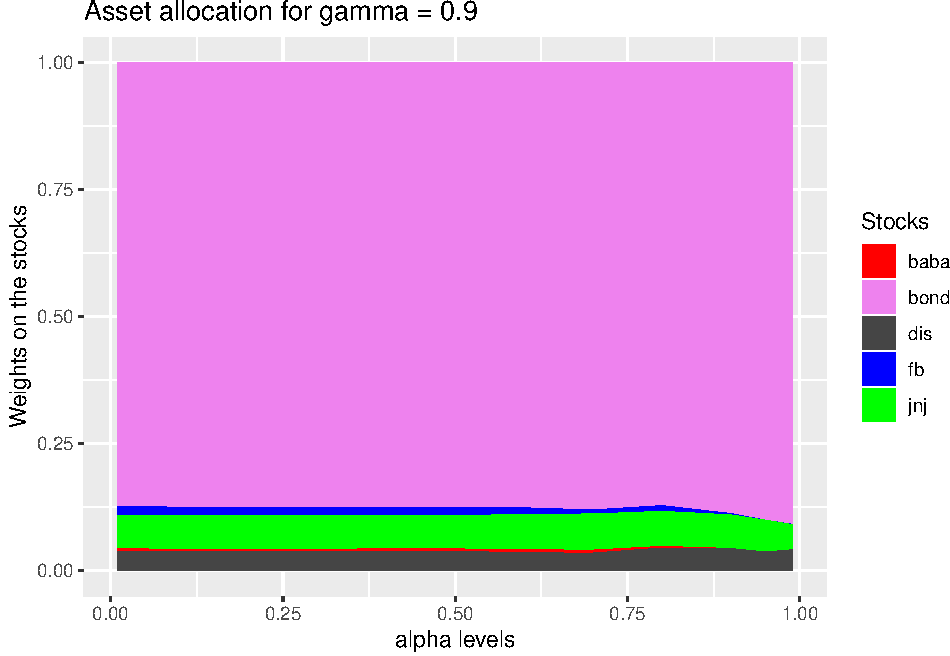
\includegraphics{Integrated_Management_Formulation_Model_files/figure-latex/unnamed-chunk-27-1.pdf}

\begin{Shaded}
\begin{Highlighting}[]
\CommentTok{# Using stacked barplots }
\KeywordTok{library}\NormalTok{(reshape2)}
\NormalTok{data9 <-}\StringTok{ }\NormalTok{resultfree9}
\KeywordTok{names}\NormalTok{(data9) <-}\StringTok{ }\KeywordTok{c}\NormalTok{(}\StringTok{"alpha"}\NormalTok{,}\StringTok{"DIS"}\NormalTok{,}\StringTok{"BABA"}\NormalTok{,}\StringTok{"JNJ"}\NormalTok{,}\StringTok{"FB"}\NormalTok{,}\StringTok{"BOND"}\NormalTok{)}
\NormalTok{mdata9 <-}\StringTok{ }\KeywordTok{melt}\NormalTok{(data9, }\DataTypeTok{id=}\KeywordTok{c}\NormalTok{(}\StringTok{"alpha"}\NormalTok{))}
\KeywordTok{names}\NormalTok{(mdata9) <-}\StringTok{ }\KeywordTok{c}\NormalTok{(}\StringTok{"Alpha"}\NormalTok{,}\StringTok{"Stocks"}\NormalTok{,}\StringTok{"Allocation"}\NormalTok{)}
\KeywordTok{ggplot}\NormalTok{() }\OperatorTok{+}\StringTok{ }\KeywordTok{geom_bar}\NormalTok{(}\KeywordTok{aes}\NormalTok{(}\DataTypeTok{y =}\NormalTok{ Allocation, }\DataTypeTok{x =}\NormalTok{ Alpha, }\DataTypeTok{fill =}\NormalTok{ Stocks), }\DataTypeTok{data =}\NormalTok{ mdata9, }\DataTypeTok{stat=}\StringTok{"identity"}\NormalTok{)}\OperatorTok{+}
\StringTok{  }\KeywordTok{scale_fill_manual}\NormalTok{(}\StringTok{"Stocks"}\NormalTok{,}\DataTypeTok{values =}
                      \KeywordTok{c}\NormalTok{(}\StringTok{"FB"}\NormalTok{=}\StringTok{"#0000FF"}\NormalTok{,}\StringTok{"JNJ"}\NormalTok{=}\StringTok{"#00FF00"}\NormalTok{,}\StringTok{"BABA"}\NormalTok{=}\StringTok{"#FF0000"}\NormalTok{,}\StringTok{"DIS"}\NormalTok{=}\StringTok{"#454545"}\NormalTok{,}\StringTok{"BOND"}\NormalTok{ =}\StringTok{ "violet"}\NormalTok{))}
\end{Highlighting}
\end{Shaded}

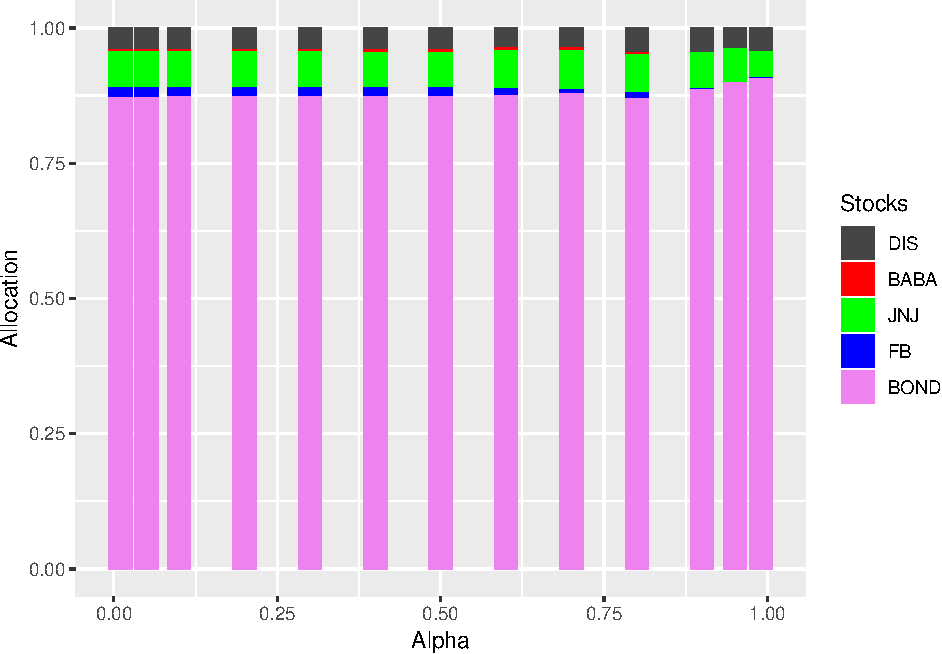
\includegraphics{Integrated_Management_Formulation_Model_files/figure-latex/unnamed-chunk-27-2.pdf}

The formation of the models almost resembles each other in the different
levels of \(\gamma\) and that is why in the different levels of
\(\gamma\), the programs almost resembles each other. Throughout the
different levels of \(\gamma\), what doesn't change is the \textbf{Amat}
matrix and so you realize that we use the same Amat matrix throughout
the programs for the different levels of \(\gamma\).

In the following, we want to just show the relationship between
\href{mailto:AV@R}{\nolinkurl{AV@R}} and
\href{mailto:V@R}{\nolinkurl{V@R}} using a standard normally distributed
data with mean = 0 and standard deviation = 1, It isn't part of this
Integrated Management Formulation model but it is just part of the
prperties of \href{mailto:AV@R}{\nolinkurl{AV@R}} as always been greater
than the \href{mailto:V@R}{\nolinkurl{V@R}} at all levels of \(\alpha\).

\subsubsection{Relationship between the Average Value-at-Risk and
Value-at-Risk}\label{relationship-between-the-average-value-at-risk-and-value-at-risk}

The following shows the relationship between Value-at-Risk and Average
Value-at-Risk for a standard normal distribution data. The main agenda
is to show that the AVaR is always greater than the VaR at all levels of
alpha.

\begin{Shaded}
\begin{Highlighting}[]
\KeywordTok{suppressMessages}\NormalTok{(}\KeywordTok{suppressWarnings}\NormalTok{(}\KeywordTok{library}\NormalTok{(QRM)))}
\NormalTok{mu =}\StringTok{ }\DecValTok{0}
\NormalTok{sigma =}\StringTok{ }\DecValTok{1}
\NormalTok{x <-}\StringTok{ }\KeywordTok{seq}\NormalTok{(}\DataTypeTok{from =} \OperatorTok{-}\DecValTok{4}\OperatorTok{*}\NormalTok{sigma, }\DataTypeTok{to =} \DecValTok{4}\OperatorTok{*}\NormalTok{sigma, }\DataTypeTok{length.out =} \DecValTok{100}\NormalTok{)}
\NormalTok{density <-}\StringTok{ }\KeywordTok{dnorm}\NormalTok{(x, }\DataTypeTok{mean =}\NormalTok{ mu, }\DataTypeTok{sd =}\NormalTok{ sigma)}
\KeywordTok{plot}\NormalTok{(x,density,}\DataTypeTok{type =} \StringTok{"l"}\NormalTok{)}

\NormalTok{VaR99 <-}\StringTok{ }\KeywordTok{qnorm}\NormalTok{(}\FloatTok{0.99}\NormalTok{, }\DataTypeTok{mean =}\NormalTok{ mu, }\DataTypeTok{sd =}\NormalTok{ sigma) }\CommentTok{#Value-at-Risk at level 99%}
\NormalTok{ES99 <-}\StringTok{ }\KeywordTok{ESnorm}\NormalTok{(}\FloatTok{0.99}\NormalTok{, }\DataTypeTok{mu =}\NormalTok{ mu, }\DataTypeTok{sd =}\NormalTok{ sigma) }\CommentTok{#Average Value-at-Risk at level 99%}

\KeywordTok{abline}\NormalTok{(}\DataTypeTok{v =}\NormalTok{ VaR99, }\DataTypeTok{col =} \StringTok{"red"}\NormalTok{)}
\KeywordTok{text}\NormalTok{(}\FloatTok{1.8}\NormalTok{,}\FloatTok{0.0}\NormalTok{, }\StringTok{"V@R0.99%"}\NormalTok{, }\DataTypeTok{col =} \StringTok{"red"}\NormalTok{) }
\KeywordTok{abline}\NormalTok{(}\DataTypeTok{v =}\NormalTok{ ES99, }\DataTypeTok{col =} \StringTok{"blue"}\NormalTok{)}
\KeywordTok{text}\NormalTok{(}\FloatTok{3.5}\NormalTok{,}\FloatTok{0.0}\NormalTok{, }\StringTok{"AV@R0.99%"}\NormalTok{, }\DataTypeTok{col =} \StringTok{"blue"}\NormalTok{) }
\end{Highlighting}
\end{Shaded}

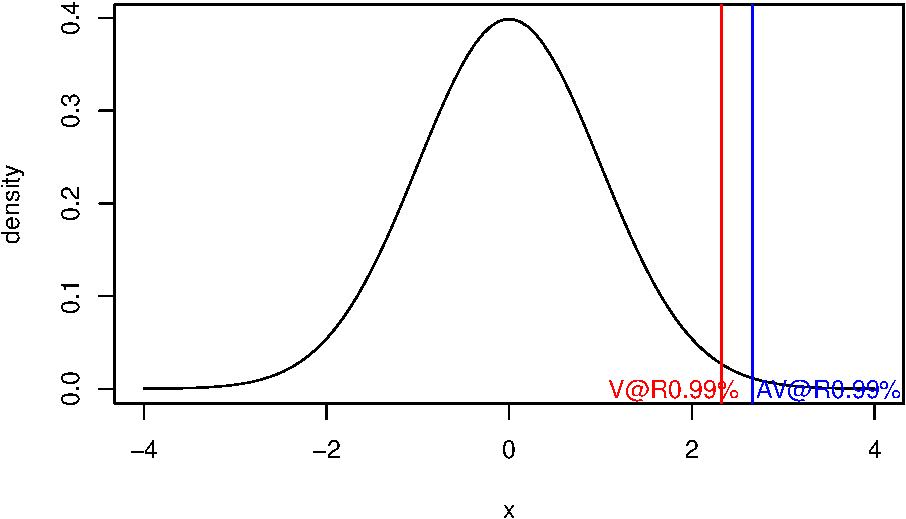
\includegraphics{Integrated_Management_Formulation_Model_files/figure-latex/unnamed-chunk-28-1.pdf}

\begin{Shaded}
\begin{Highlighting}[]
\NormalTok{var <-}\StringTok{ }\KeywordTok{vector}\NormalTok{(}\DataTypeTok{mode =} \StringTok{"numeric"}\NormalTok{)}
\NormalTok{avar <-}\StringTok{ }\KeywordTok{vector}\NormalTok{(}\DataTypeTok{mode =} \StringTok{"numeric"}\NormalTok{)}
\NormalTok{alpha <-}\StringTok{ }\KeywordTok{c}\NormalTok{(}\FloatTok{0.0}\NormalTok{,}\FloatTok{0.05}\NormalTok{,}\FloatTok{0.1}\NormalTok{,}\FloatTok{0.2}\NormalTok{,}\FloatTok{0.3}\NormalTok{,}\FloatTok{0.4}\NormalTok{,}\FloatTok{0.5}\NormalTok{,}\FloatTok{0.6}\NormalTok{,}\FloatTok{0.7}\NormalTok{,}\FloatTok{0.8}\NormalTok{,}\FloatTok{0.90}\NormalTok{,}\FloatTok{0.95}\NormalTok{,}\FloatTok{0.99}\NormalTok{)}
\ControlFlowTok{for}\NormalTok{ (alp }\ControlFlowTok{in}\NormalTok{ alpha)\{}
\NormalTok{  var <-}\StringTok{ }\KeywordTok{append}\NormalTok{(var,}\KeywordTok{qnorm}\NormalTok{(alp,}\DataTypeTok{mean =}\NormalTok{ mu, }\DataTypeTok{sd =}\NormalTok{ sigma))}
\NormalTok{  avar <-}\StringTok{ }\KeywordTok{append}\NormalTok{(avar,}\KeywordTok{ESnorm}\NormalTok{(alp,}\DataTypeTok{mu =}\NormalTok{ mu , }\DataTypeTok{sd =}\NormalTok{ sigma))}
\NormalTok{\}}
\KeywordTok{plot}\NormalTok{(alpha,var,}\DataTypeTok{type=}\StringTok{"l"}\NormalTok{, }\DataTypeTok{col=}\StringTok{"green"}\NormalTok{, }\DataTypeTok{xlab =} \KeywordTok{expression}\NormalTok{(alpha), }\DataTypeTok{ylab =} \StringTok{"V@R and AV@R"}\NormalTok{,}\DataTypeTok{lwd =} \DecValTok{2}\NormalTok{)}
\KeywordTok{lines}\NormalTok{(alpha,avar,}\DataTypeTok{col =} \StringTok{"red"}\NormalTok{,}\DataTypeTok{lwd =} \DecValTok{2}\NormalTok{)}
\end{Highlighting}
\end{Shaded}

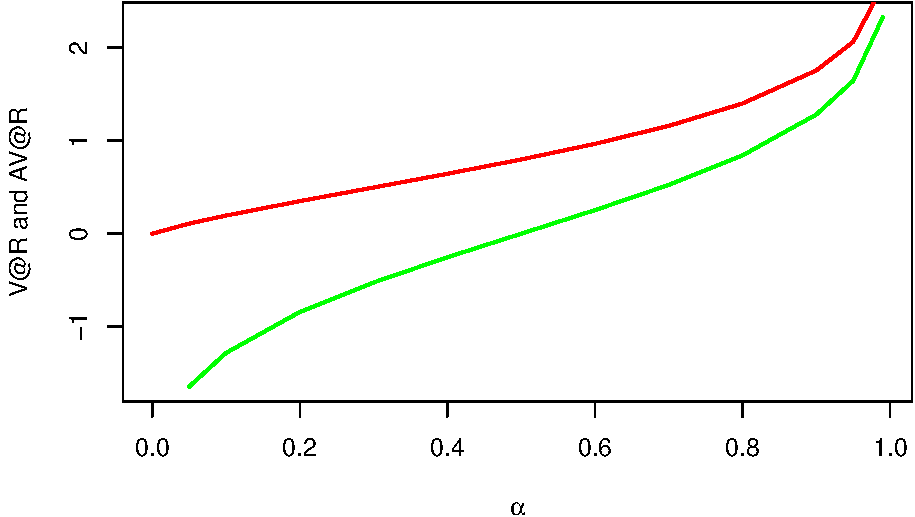
\includegraphics{Integrated_Management_Formulation_Model_files/figure-latex/unnamed-chunk-28-2.pdf}


\end{document}
